\documentclass{book}
\usepackage[a4paper,top=2.5cm,bottom=2.5cm,left=2.5cm,right=2.5cm]{geometry}
\usepackage{makeidx}
\usepackage{natbib}
\usepackage{graphicx}
\usepackage{multicol}
\usepackage{float}
\usepackage{listings}
\usepackage{color}
\usepackage{ifthen}
\usepackage[table]{xcolor}
\usepackage{textcomp}
\usepackage{alltt}
\usepackage{ifpdf}
\ifpdf
\usepackage[pdftex,
            pagebackref=true,
            colorlinks=true,
            linkcolor=blue,
            unicode
           ]{hyperref}
\else
\usepackage[ps2pdf,
            pagebackref=true,
            colorlinks=true,
            linkcolor=blue,
            unicode
           ]{hyperref}
\usepackage{pspicture}
\fi
\usepackage[utf8]{inputenc}
\usepackage{mathptmx}
\usepackage[scaled=.90]{helvet}
\usepackage{courier}
\usepackage{sectsty}
\usepackage{amssymb}
\usepackage[titles]{tocloft}
\usepackage{doxygen}
\lstset{language=C++,inputencoding=utf8,basicstyle=\footnotesize,breaklines=true,breakatwhitespace=true,tabsize=4,numbers=left }
\makeindex
\setcounter{tocdepth}{3}
\renewcommand{\footrulewidth}{0.4pt}
\renewcommand{\familydefault}{\sfdefault}
\hfuzz=15pt
\setlength{\emergencystretch}{15pt}
\hbadness=750
\tolerance=750
\begin{document}
\hypersetup{pageanchor=false,citecolor=blue}
\begin{titlepage}
\vspace*{7cm}
\begin{center}
{\Large C\-B\-E\-M\-D\-: Parallelized M\-D in Various Thermodynamic Ensembles }\\
\vspace*{1cm}
{\large Generated by Doxygen 1.8.2}\\
\vspace*{0.5cm}
{\small Fri Jan 18 2013 00:07:23}\\
\end{center}
\end{titlepage}
\clearemptydoublepage
\pagenumbering{roman}
\tableofcontents
\clearemptydoublepage
\pagenumbering{arabic}
\hypersetup{pageanchor=true,citecolor=blue}
\chapter{Hierarchical Index}
\section{Class Hierarchy}
This inheritance list is sorted roughly, but not completely, alphabetically\-:\begin{DoxyCompactList}
\item \contentsline{section}{atom\-:\-:Atom}{\pageref{structatom_1_1Atom}}{}
\item exception\begin{DoxyCompactList}
\item \contentsline{section}{Fene\-Exception}{\pageref{classFeneException}}{}
\item \contentsline{section}{Slj\-Exception}{\pageref{classSljException}}{}
\end{DoxyCompactList}
\item \contentsline{section}{integrator\-:\-:Integrator}{\pageref{classintegrator_1_1Integrator}}{}
\begin{DoxyCompactList}
\item \contentsline{section}{integrator\-:\-:Andersen}{\pageref{classintegrator_1_1Andersen}}{}
\item \contentsline{section}{integrator\-:\-:N\-H\-A}{\pageref{classintegrator_1_1NHA}}{}
\item \contentsline{section}{integrator\-:\-:Nose\-Hoover}{\pageref{classintegrator_1_1NoseHoover}}{}
\item \contentsline{section}{integrator\-:\-:Velocity\-\_\-verlet}{\pageref{classintegrator_1_1Velocity__verlet}}{}
\item \contentsline{section}{integrator\-:\-:Verlet}{\pageref{classintegrator_1_1Verlet}}{}
\end{DoxyCompactList}
\item \contentsline{section}{Interaction}{\pageref{classInteraction}}{}
\item \contentsline{section}{sim\-\_\-system\-:\-:System}{\pageref{classsim__system_1_1System}}{}
\item Test\begin{DoxyCompactList}
\item \contentsline{section}{Atom\-Energy}{\pageref{classAtomEnergy}}{}
\item \contentsline{section}{Many\-Body\-Test}{\pageref{classManyBodyTest}}{}
\item \contentsline{section}{Two\-Body\-Test}{\pageref{classTwoBodyTest}}{}
\end{DoxyCompactList}
\end{DoxyCompactList}

\chapter{Class Index}
\section{Class List}
Here are the classes, structs, unions and interfaces with brief descriptions\-:\begin{DoxyCompactList}
\item\contentsline{section}{\hyperlink{classAndersen}{Andersen} \\*N\-V\-T, \hyperlink{classAndersen}{Andersen} thermostat Run (i.\-e. integrate) a system forward in time for a specified number of timesteps }{\pageref{classAndersen}}{}
\item\contentsline{section}{\hyperlink{structAtom}{Atom} \\*\hyperlink{structAtom}{Atom} class is defined as a struct so as to be easy to pass with M\-P\-I }{\pageref{structAtom}}{}
\item\contentsline{section}{\hyperlink{classFeneException}{Fene\-Exception} \\*Fene exception class is thrown if there is an error }{\pageref{classFeneException}}{}
\item\contentsline{section}{\hyperlink{classIntegrator}{Integrator} \\*$<$ Abstract base class for integrators }{\pageref{classIntegrator}}{}
\item\contentsline{section}{\hyperlink{classInteraction}{Interaction} \\*This class stores how a pair of particles interacts }{\pageref{classInteraction}}{}
\item\contentsline{section}{\hyperlink{classSljException}{Slj\-Exception} \\*S\-L\-J exception class is thrown if there is an error }{\pageref{classSljException}}{}
\item\contentsline{section}{\hyperlink{classSystem}{System} }{\pageref{classSystem}}{}
\item\contentsline{section}{\hyperlink{classVerlet}{Verlet} \\*N\-V\-E, \hyperlink{classVerlet}{Verlet} }{\pageref{classVerlet}}{}
\end{DoxyCompactList}

\chapter{File Index}
\section{File List}
Here is a list of all documented files with brief descriptions\-:\begin{DoxyCompactList}
\item\contentsline{section}{\hyperlink{andersen_8cpp}{andersen.\-cpp} \\*Driver for M\-P\-I Version of C\-B\-E\-M\-D with \hyperlink{classAndersen}{Andersen} Thermostat }{\pageref{andersen_8cpp}}{}
\item\contentsline{section}{\hyperlink{atom_8cpp}{atom.\-cpp} \\*Functions for handling M\-D \hyperlink{structAtom}{Atom} Information }{\pageref{atom_8cpp}}{}
\item\contentsline{section}{\hyperlink{atom_8h}{atom.\-h} \\*M\-D \hyperlink{structAtom}{Atom} Information }{\pageref{atom_8h}}{}
\item\contentsline{section}{\hyperlink{CBEMD_8h}{C\-B\-E\-M\-D.\-h} \\*Header grouping source headers into one simple header for the driver program(s) }{\pageref{CBEMD_8h}}{}
\item\contentsline{section}{\hyperlink{common_8h}{common.\-h} \\*Header that lumps all common header files into one }{\pageref{common_8h}}{}
\item\contentsline{section}{\hyperlink{domain__decomp_8cpp}{domain\-\_\-decomp.\-cpp} \\*Source code containing functions for performing domain decomposition }{\pageref{domain__decomp_8cpp}}{}
\item\contentsline{section}{\hyperlink{domain__decomp_8h}{domain\-\_\-decomp.\-h} \\*Header file for domain decomposition }{\pageref{domain__decomp_8h}}{}
\item\contentsline{section}{\hyperlink{force__calc_8cpp}{force\-\_\-calc.\-cpp} \\*Source code for force calculation }{\pageref{force__calc_8cpp}}{}
\item\contentsline{section}{\hyperlink{force__calc_8h}{force\-\_\-calc.\-h} \\*Header for force\-\_\-calc function }{\pageref{force__calc_8h}}{}
\item\contentsline{section}{\hyperlink{global_8h}{global.\-h} \\*Global variables }{\pageref{global_8h}}{}
\item\contentsline{section}{\hyperlink{initialize_8cpp}{initialize.\-cpp} \\*Initialization routines for \hyperlink{classSystem}{System} object, as well as finalization of M\-P\-I }{\pageref{initialize_8cpp}}{}
\item\contentsline{section}{{\bfseries initialize.\-h} }{\pageref{initialize_8h}}{}
\item\contentsline{section}{\hyperlink{integrator_8cpp}{integrator.\-cpp} \\*M\-D Integrator(s) Information }{\pageref{integrator_8cpp}}{}
\item\contentsline{section}{\hyperlink{integrator_8h}{integrator.\-h} \\*M\-D Integrator(s) Information }{\pageref{integrator_8h}}{}
\item\contentsline{section}{\hyperlink{interaction_8cpp}{interaction.\-cpp} \\*Source code for interaction functions }{\pageref{interaction_8cpp}}{}
\item\contentsline{section}{\hyperlink{interaction_8h}{interaction.\-h} \\*Header file for interaction information }{\pageref{interaction_8h}}{}
\item\contentsline{section}{\hyperlink{misc_8cpp}{misc.\-cpp} \\*Source code for miscellaneous routines }{\pageref{misc_8cpp}}{}
\item\contentsline{section}{\hyperlink{misc_8h}{misc.\-h} \\*Header for Miscellaneous Routines }{\pageref{misc_8h}}{}
\item\contentsline{section}{\hyperlink{mpiatom_8h}{mpiatom.\-h} }{\pageref{mpiatom_8h}}{}
\item\contentsline{section}{\hyperlink{read__interaction_8cpp}{read\-\_\-interaction.\-cpp} \\*Source code to read in interaction parameters from a parameter file }{\pageref{read__interaction_8cpp}}{}
\item\contentsline{section}{\hyperlink{read__interaction_8h}{read\-\_\-interaction.\-h} \\*Header file for reading interactions in }{\pageref{read__interaction_8h}}{}
\item\contentsline{section}{\hyperlink{read__xml_8cpp}{read\-\_\-xml.\-cpp} \\*I/\-O for X\-M\-L file format }{\pageref{read__xml_8cpp}}{}
\item\contentsline{section}{\hyperlink{read__xml_8h}{read\-\_\-xml.\-h} \\*I/\-O for X\-M\-L }{\pageref{read__xml_8h}}{}
\item\contentsline{section}{\hyperlink{system_8cpp}{system.\-cpp} \\*Source code for the \hyperlink{classSystem}{System} object }{\pageref{system_8cpp}}{}
\item\contentsline{section}{\hyperlink{system_8h}{system.\-h} \\*Header for M\-D \hyperlink{classSystem}{System} Information }{\pageref{system_8h}}{}
\item\contentsline{section}{\hyperlink{verlet_8cpp}{verlet.\-cpp} \\*Driver for M\-P\-I Version of C\-B\-E\-M\-D verlet }{\pageref{verlet_8cpp}}{}
\end{DoxyCompactList}

\chapter{Class Documentation}
\hypertarget{classAndersen}{\section{Andersen Class Reference}
\label{classAndersen}\index{Andersen@{Andersen}}
}


N\-V\-T, \hyperlink{classAndersen}{Andersen} thermostat Run (i.\-e. integrate) a system forward in time for a specified number of timesteps.  




{\ttfamily \#include $<$integrator.\-h$>$}

Inheritance diagram for Andersen\-:\begin{figure}[H]
\begin{center}
\leavevmode
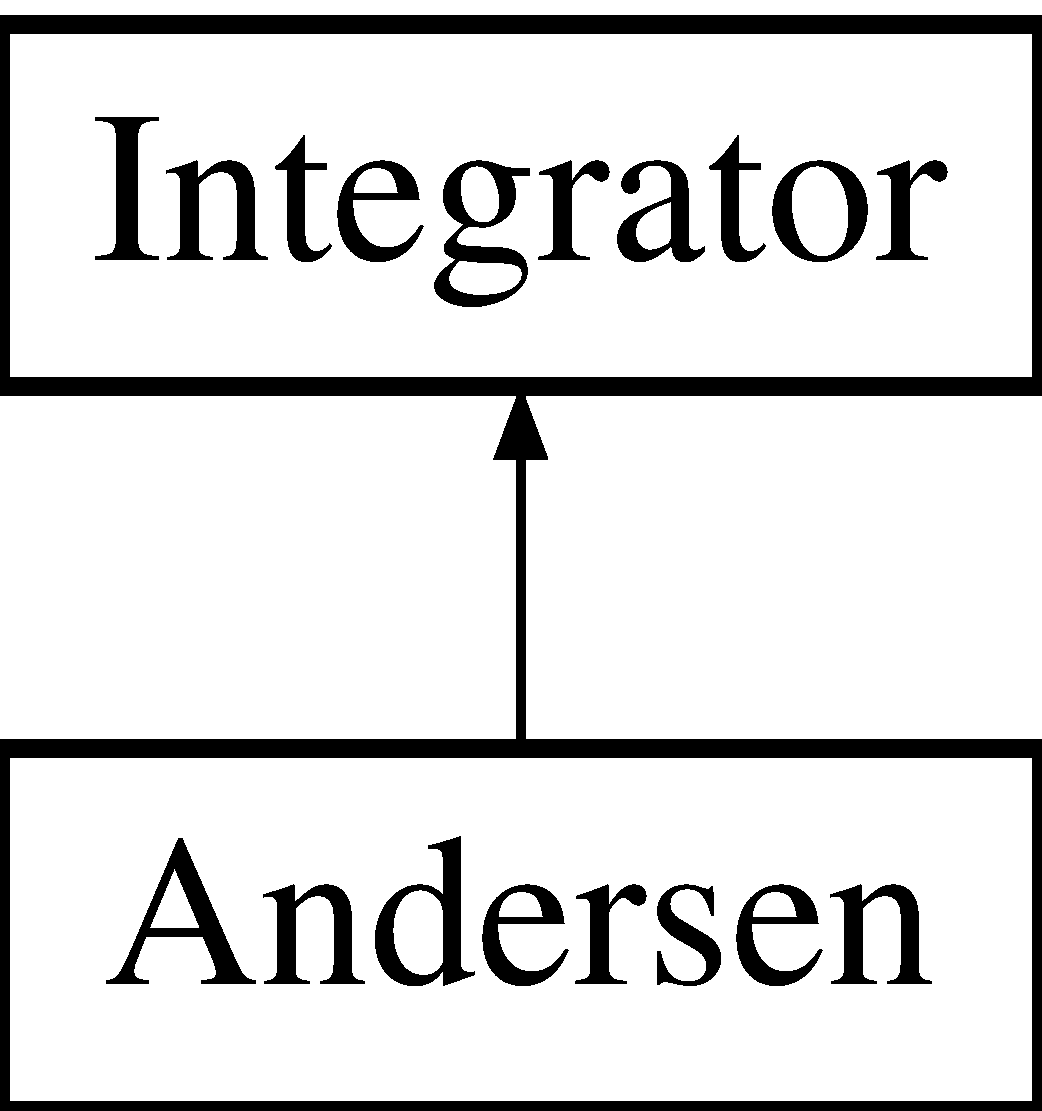
\includegraphics[height=2.000000cm]{classAndersen}
\end{center}
\end{figure}
\subsection*{Public Member Functions}
\begin{DoxyCompactItemize}
\item 
\hyperlink{classAndersen_a1234214695cde894eb0f3da49e63b53f}{Andersen} (double deltat, double temp, double nu)
\item 
\hypertarget{classAndersen_a600ded26c24fb099880be97e1bf6b778}{void {\bfseries set\-\_\-temp} (double temp)}\label{classAndersen_a600ded26c24fb099880be97e1bf6b778}

\item 
\hypertarget{classAndersen_acba0beac53d9fd9de7ac607c0b5d530e}{double {\bfseries get\-Temp} () const }\label{classAndersen_acba0beac53d9fd9de7ac607c0b5d530e}

\item 
\hypertarget{classAndersen_a5316d4c5545689208f69a371bacf5664}{double {\bfseries getdt} ()}\label{classAndersen_a5316d4c5545689208f69a371bacf5664}

\item 
int \hyperlink{classAndersen_a0d61b4c49eba214fdf38af544758d9cc}{step} (\hyperlink{classSystem}{System} $\ast$sys)
\item 
\hypertarget{classAndersen_a6ee278d57758012c461219202b88c91b}{double {\bfseries nu} () const }\label{classAndersen_a6ee278d57758012c461219202b88c91b}

\end{DoxyCompactItemize}
\subsection*{Additional Inherited Members}


\subsection{Detailed Description}
N\-V\-T, \hyperlink{classAndersen}{Andersen} thermostat Run (i.\-e. integrate) a system forward in time for a specified number of timesteps. 

\subsection{Constructor \& Destructor Documentation}
\hypertarget{classAndersen_a1234214695cde894eb0f3da49e63b53f}{\index{Andersen@{Andersen}!Andersen@{Andersen}}
\index{Andersen@{Andersen}!Andersen@{Andersen}}
\subsubsection[{Andersen}]{\setlength{\rightskip}{0pt plus 5cm}Andersen\-::\-Andersen (
\begin{DoxyParamCaption}
\item[{double}]{deltat, }
\item[{double}]{temp, }
\item[{double}]{nu}
\end{DoxyParamCaption}
)}}\label{classAndersen_a1234214695cde894eb0f3da49e63b53f}

\begin{DoxyParams}[1]{Parameters}
\mbox{\tt in}  & {\em deltat} & Incremental timestep \\
\hline
\mbox{\tt in}  & {\em temp} & Set point temperature \\
\hline
\end{DoxyParams}


\subsection{Member Function Documentation}
\hypertarget{classAndersen_a0d61b4c49eba214fdf38af544758d9cc}{\index{Andersen@{Andersen}!step@{step}}
\index{step@{step}!Andersen@{Andersen}}
\subsubsection[{step}]{\setlength{\rightskip}{0pt plus 5cm}int Andersen\-::step (
\begin{DoxyParamCaption}
\item[{{\bf System} $\ast$}]{sys}
\end{DoxyParamCaption}
)\hspace{0.3cm}{\ttfamily [virtual]}}}\label{classAndersen_a0d61b4c49eba214fdf38af544758d9cc}
Step forward one timestep with the \hyperlink{classAndersen}{Andersen} thermostat. This reports the instantaneous temperature after each step. 
\begin{DoxyParams}[1]{Parameters}
\mbox{\tt in}  & {\em $\ast$sys} & Pointer to \hyperlink{classSystem}{System} to integrate. \\
\hline
\end{DoxyParams}


Implements \hyperlink{classIntegrator_aac53df432f961f8661e157b2a86d8b31}{Integrator}.



The documentation for this class was generated from the following files\-:\begin{DoxyCompactItemize}
\item 
\hyperlink{integrator_8h}{integrator.\-h}\item 
\hyperlink{integrator_8cpp}{integrator.\-cpp}\end{DoxyCompactItemize}

\hypertarget{structAtom}{\section{Atom Struct Reference}
\label{structAtom}\index{Atom@{Atom}}
}


\hyperlink{structAtom}{Atom} class is defined as a struct so as to be easy to pass with M\-P\-I.  




{\ttfamily \#include $<$atom.\-h$>$}

\subsection*{Public Attributes}
\begin{DoxyCompactItemize}
\item 
\hypertarget{structAtom_a99bc3071c5e17dd454c6257dce692a2a}{double \hyperlink{structAtom_a99bc3071c5e17dd454c6257dce692a2a}{pos} \mbox{[}\hyperlink{global_8h_ac92befc9e919a4caa991cbddc2455f6a}{N\-D\-I\-M}\mbox{]}}\label{structAtom_a99bc3071c5e17dd454c6257dce692a2a}

\begin{DoxyCompactList}\small\item\em Cartesian coordinates. \end{DoxyCompactList}\item 
\hypertarget{structAtom_a5ab233568e9091c7acdfef42efcd933c}{double \hyperlink{structAtom_a5ab233568e9091c7acdfef42efcd933c}{prev\-\_\-pos} \mbox{[}\hyperlink{global_8h_ac92befc9e919a4caa991cbddc2455f6a}{N\-D\-I\-M}\mbox{]}}\label{structAtom_a5ab233568e9091c7acdfef42efcd933c}

\begin{DoxyCompactList}\small\item\em Cartesian coordinates for the previous position of the atom (needed for integrator) \end{DoxyCompactList}\item 
\hypertarget{structAtom_afe6686a5403e25e7fe0e64f6623547ba}{double \hyperlink{structAtom_afe6686a5403e25e7fe0e64f6623547ba}{vel} \mbox{[}\hyperlink{global_8h_ac92befc9e919a4caa991cbddc2455f6a}{N\-D\-I\-M}\mbox{]}}\label{structAtom_afe6686a5403e25e7fe0e64f6623547ba}

\begin{DoxyCompactList}\small\item\em Cartesian velocities (vx, vy, vz) \end{DoxyCompactList}\item 
\hypertarget{structAtom_afcf18b786e37ff87a7d781c5e333ef40}{double \hyperlink{structAtom_afcf18b786e37ff87a7d781c5e333ef40}{force} \mbox{[}\hyperlink{global_8h_ac92befc9e919a4caa991cbddc2455f6a}{N\-D\-I\-M}\mbox{]}}\label{structAtom_afcf18b786e37ff87a7d781c5e333ef40}

\begin{DoxyCompactList}\small\item\em Cartesian force, (fx, fy, fz) \end{DoxyCompactList}\item 
\hypertarget{structAtom_a90e6f00ca3ae2fda9b87cb27aac5929d}{double \hyperlink{structAtom_a90e6f00ca3ae2fda9b87cb27aac5929d}{mass}}\label{structAtom_a90e6f00ca3ae2fda9b87cb27aac5929d}

\begin{DoxyCompactList}\small\item\em Atomic mass (in reduced units) \end{DoxyCompactList}\item 
\hypertarget{structAtom_adc9135600cf2007211e760b6005e1a18}{double \hyperlink{structAtom_adc9135600cf2007211e760b6005e1a18}{diam}}\label{structAtom_adc9135600cf2007211e760b6005e1a18}

\begin{DoxyCompactList}\small\item\em Atomic diameter (in reduced units) \end{DoxyCompactList}\item 
\hypertarget{structAtom_a7c2770b985ea2d1615ab750fba4d45b8}{int \hyperlink{structAtom_a7c2770b985ea2d1615ab750fba4d45b8}{type}}\label{structAtom_a7c2770b985ea2d1615ab750fba4d45b8}

\begin{DoxyCompactList}\small\item\em Internally indexed type of this atom. \end{DoxyCompactList}\item 
\hypertarget{structAtom_a7a297229ec0e4988ee6620f2caf3f572}{int \hyperlink{structAtom_a7a297229ec0e4988ee6620f2caf3f572}{sys\-\_\-index}}\label{structAtom_a7a297229ec0e4988ee6620f2caf3f572}

\begin{DoxyCompactList}\small\item\em Global atom index, i.\-e. unique in the system. \end{DoxyCompactList}\end{DoxyCompactItemize}


\subsection{Detailed Description}
\hyperlink{structAtom}{Atom} class is defined as a struct so as to be easy to pass with M\-P\-I. 

The documentation for this struct was generated from the following file\-:\begin{DoxyCompactItemize}
\item 
\hyperlink{atom_8h}{atom.\-h}\end{DoxyCompactItemize}

\hypertarget{classFeneException}{\section{Fene\-Exception Class Reference}
\label{classFeneException}\index{Fene\-Exception@{Fene\-Exception}}
}


Fene exception class is thrown if there is an error.  




{\ttfamily \#include $<$interaction.\-h$>$}

Inheritance diagram for Fene\-Exception\-:\begin{figure}[H]
\begin{center}
\leavevmode
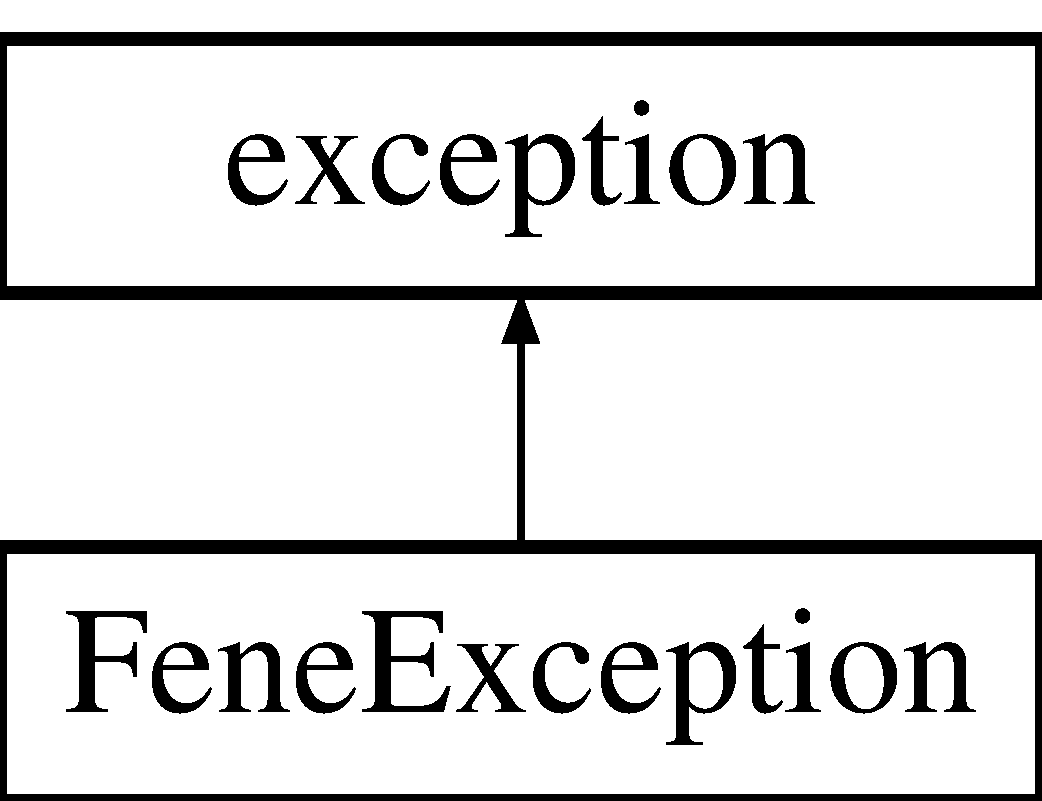
\includegraphics[height=2.000000cm]{classFeneException}
\end{center}
\end{figure}
\subsection*{Public Member Functions}
\begin{DoxyCompactItemize}
\item 
\hypertarget{classFeneException_a0c49ab4b1d3554ac7520516fef599c70}{{\bfseries Fene\-Exception} (const int ind1, const int ind2, const double dist, const double r0)}\label{classFeneException_a0c49ab4b1d3554ac7520516fef599c70}

\item 
\hypertarget{classFeneException_ad9722b7db057f1b70d33e2e394e168af}{virtual const char $\ast$ {\bfseries what} () const   throw ()}\label{classFeneException_ad9722b7db057f1b70d33e2e394e168af}

\end{DoxyCompactItemize}
\subsection*{Protected Attributes}
\begin{DoxyCompactItemize}
\item 
\hypertarget{classFeneException_aa1f88371f02cca1c4fc16e8e3300b1ba}{int {\bfseries ind1\-\_\-}}\label{classFeneException_aa1f88371f02cca1c4fc16e8e3300b1ba}

\item 
\hypertarget{classFeneException_a723fb7fca56d3c0427a484e7a25180ef}{int {\bfseries ind2\-\_\-}}\label{classFeneException_a723fb7fca56d3c0427a484e7a25180ef}

\item 
\hypertarget{classFeneException_a4a3752aa9e4bd86e8244cb95c76ba713}{double {\bfseries dist\-\_\-}}\label{classFeneException_a4a3752aa9e4bd86e8244cb95c76ba713}

\item 
\hypertarget{classFeneException_adb4d7db732aa4a784fa2c4ec0c68744d}{double {\bfseries r0\-\_\-}}\label{classFeneException_adb4d7db732aa4a784fa2c4ec0c68744d}

\end{DoxyCompactItemize}


\subsection{Detailed Description}
Fene exception class is thrown if there is an error. 

The documentation for this class was generated from the following file\-:\begin{DoxyCompactItemize}
\item 
\hyperlink{interaction_8h}{interaction.\-h}\end{DoxyCompactItemize}

\hypertarget{classIntegrator}{\section{Integrator Class Reference}
\label{classIntegrator}\index{Integrator@{Integrator}}
}


$<$ Abstract base class for integrators  




{\ttfamily \#include $<$integrator.\-h$>$}

Inheritance diagram for Integrator\-:\begin{figure}[H]
\begin{center}
\leavevmode
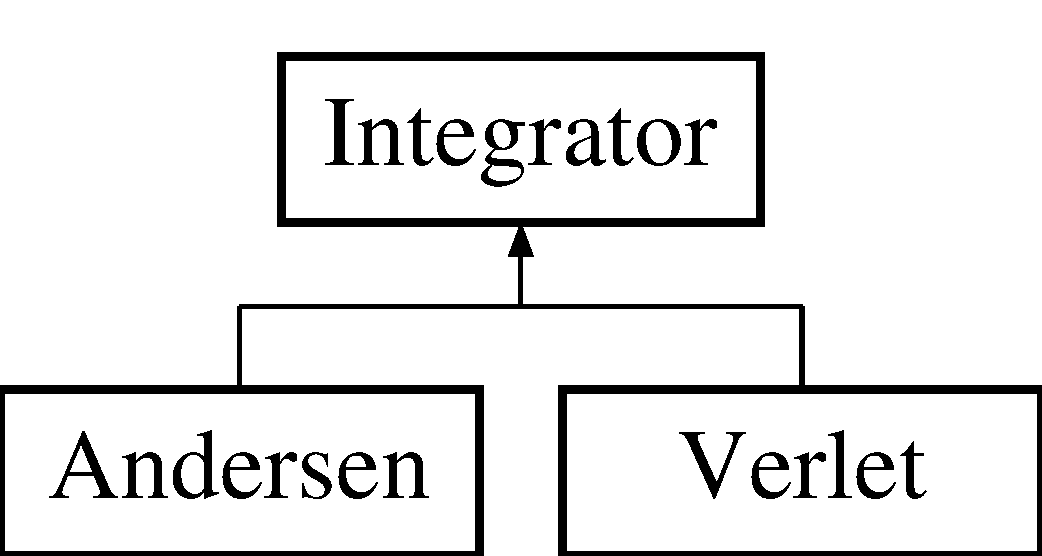
\includegraphics[height=2.000000cm]{classIntegrator}
\end{center}
\end{figure}
\subsection*{Public Member Functions}
\begin{DoxyCompactItemize}
\item 
\hypertarget{classIntegrator_ae8a6ce5dbc5a6bf468fb151a9f9c79f1}{void {\bfseries set\-\_\-dt} (const double dt)}\label{classIntegrator_ae8a6ce5dbc5a6bf468fb151a9f9c79f1}

\item 
\hypertarget{classIntegrator_a63fb8d0a5c43c9c5cb609a39728fdb27}{double {\bfseries dt} () const }\label{classIntegrator_a63fb8d0a5c43c9c5cb609a39728fdb27}

\item 
\hypertarget{classIntegrator_a46707a9735b94ffcb503709fb595fe9a}{void {\bfseries set\-\_\-temp} (double temp)}\label{classIntegrator_a46707a9735b94ffcb503709fb595fe9a}

\item 
\hypertarget{classIntegrator_a0494a27296817ff78ce6614f2f5ad50e}{double {\bfseries get\-Temp} () const }\label{classIntegrator_a0494a27296817ff78ce6614f2f5ad50e}

\item 
\hypertarget{classIntegrator_aac53df432f961f8661e157b2a86d8b31}{virtual int \hyperlink{classIntegrator_aac53df432f961f8661e157b2a86d8b31}{step} (\hyperlink{classSystem}{System} $\ast$sys)=0}\label{classIntegrator_aac53df432f961f8661e157b2a86d8b31}

\begin{DoxyCompactList}\small\item\em Requires all subclasses to be able to execute a step. \end{DoxyCompactList}\end{DoxyCompactItemize}
\subsection*{Protected Attributes}
\begin{DoxyCompactItemize}
\item 
\hypertarget{classIntegrator_a26e3530cd1b2c3cf844d550b317568a9}{double {\bfseries dt\-\_\-}}\label{classIntegrator_a26e3530cd1b2c3cf844d550b317568a9}

\item 
\hypertarget{classIntegrator_a37fee941833e7d7d60c200d82160139f}{double {\bfseries temp\-\_\-}}\label{classIntegrator_a37fee941833e7d7d60c200d82160139f}

\end{DoxyCompactItemize}


\subsection{Detailed Description}
$<$ Abstract base class for integrators 

The step function should return S\-A\-F\-E\-\_\-\-E\-X\-I\-T if successfully executed, integer error flag otherwise. 

The documentation for this class was generated from the following file\-:\begin{DoxyCompactItemize}
\item 
\hyperlink{integrator_8h}{integrator.\-h}\end{DoxyCompactItemize}

\hypertarget{classInteraction}{\section{Interaction Class Reference}
\label{classInteraction}\index{Interaction@{Interaction}}
}


This class stores how a pair of particles interacts.  




{\ttfamily \#include $<$interaction.\-h$>$}

\subsection*{Public Member Functions}
\begin{DoxyCompactItemize}
\item 
\hypertarget{classInteraction_ac130c083d3ebb298daa2b65c23bdf6f5}{double \hyperlink{classInteraction_ac130c083d3ebb298daa2b65c23bdf6f5}{force\-\_\-energy} (\hyperlink{structatom_1_1Atom}{Atom} $\ast$a1, \hyperlink{structatom_1_1Atom}{Atom} $\ast$a2, const vector$<$ double $>$ $\ast$box)}\label{classInteraction_ac130c083d3ebb298daa2b65c23bdf6f5}

\begin{DoxyCompactList}\small\item\em Computes force (stored on atoms) and energy (returned) \end{DoxyCompactList}\item 
\hypertarget{classInteraction_a4c47992e9d1f5108bdededb441a2936e}{void \hyperlink{classInteraction_a4c47992e9d1f5108bdededb441a2936e}{set\-\_\-force\-\_\-energy} (force\-\_\-energy\-\_\-ptr ife)}\label{classInteraction_a4c47992e9d1f5108bdededb441a2936e}

\begin{DoxyCompactList}\small\item\em Assign the potential calculator. \end{DoxyCompactList}\item 
\hypertarget{classInteraction_a28f5616df90a267d61bf02d2f767de30}{void \hyperlink{classInteraction_a28f5616df90a267d61bf02d2f767de30}{set\-\_\-args} (const vector$<$ double $>$ args)}\label{classInteraction_a28f5616df90a267d61bf02d2f767de30}

\begin{DoxyCompactList}\small\item\em Assign energy and force arguments. \end{DoxyCompactList}\item 
\hypertarget{classInteraction_a28a9c76d26d78acaf9a8112850b2a1d8}{force\-\_\-energy\-\_\-ptr \hyperlink{classInteraction_a28a9c76d26d78acaf9a8112850b2a1d8}{check\-\_\-force\-\_\-energy\-\_\-function} () const }\label{classInteraction_a28a9c76d26d78acaf9a8112850b2a1d8}

\begin{DoxyCompactList}\small\item\em Return the function for force and energy calculations. \end{DoxyCompactList}\end{DoxyCompactItemize}


\subsection{Detailed Description}
This class stores how a pair of particles interacts. 

Returns energy and force as long as r $<$ r\-\_\-\{cut\}, else 0. 

The documentation for this class was generated from the following file\-:\begin{DoxyCompactItemize}
\item 
\hyperlink{interaction_8h}{interaction.\-h}\end{DoxyCompactItemize}

\hypertarget{classSljException}{\section{Slj\-Exception Class Reference}
\label{classSljException}\index{Slj\-Exception@{Slj\-Exception}}
}


S\-L\-J exception class is thrown if there is an error.  




{\ttfamily \#include $<$interaction.\-h$>$}

Inheritance diagram for Slj\-Exception\-:\begin{figure}[H]
\begin{center}
\leavevmode
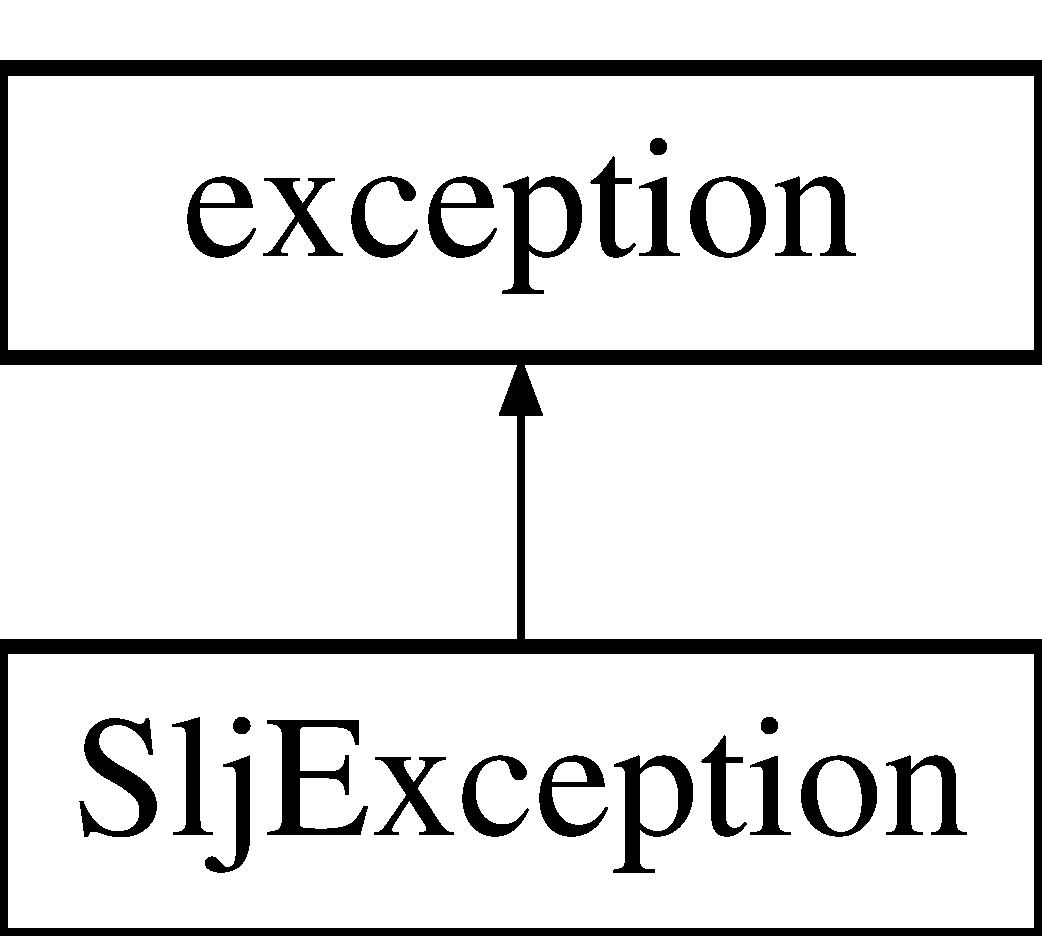
\includegraphics[height=2.000000cm]{classSljException}
\end{center}
\end{figure}
\subsection*{Public Member Functions}
\begin{DoxyCompactItemize}
\item 
\hypertarget{classSljException_a844c40d1317e90d796cc5224d6bf9f5b}{{\bfseries Slj\-Exception} (const int ind1, const int ind2, const double dist, const double delta)}\label{classSljException_a844c40d1317e90d796cc5224d6bf9f5b}

\item 
\hypertarget{classSljException_a1e5587bb78df07885ce111a7e6d4295a}{virtual const char $\ast$ {\bfseries what} () const   throw ()}\label{classSljException_a1e5587bb78df07885ce111a7e6d4295a}

\end{DoxyCompactItemize}
\subsection*{Protected Attributes}
\begin{DoxyCompactItemize}
\item 
\hypertarget{classSljException_aa5ae091f4f5cc401ecdb838b6f4e3be9}{int {\bfseries ind1\-\_\-}}\label{classSljException_aa5ae091f4f5cc401ecdb838b6f4e3be9}

\item 
\hypertarget{classSljException_af37b08ff37b7c1e43e4e80342766e41e}{int {\bfseries ind2\-\_\-}}\label{classSljException_af37b08ff37b7c1e43e4e80342766e41e}

\item 
\hypertarget{classSljException_aeb9853dfd402e4541b50415915fabe50}{double {\bfseries dist\-\_\-}}\label{classSljException_aeb9853dfd402e4541b50415915fabe50}

\item 
\hypertarget{classSljException_a02625514011528a6f3f7516d2af33035}{double {\bfseries delta\-\_\-}}\label{classSljException_a02625514011528a6f3f7516d2af33035}

\end{DoxyCompactItemize}


\subsection{Detailed Description}
S\-L\-J exception class is thrown if there is an error. 

The documentation for this class was generated from the following file\-:\begin{DoxyCompactItemize}
\item 
\hyperlink{interaction_8h}{interaction.\-h}\end{DoxyCompactItemize}

\hypertarget{classSystem}{\section{System Class Reference}
\label{classSystem}\index{System@{System}}
}
\subsection*{Public Member Functions}
\begin{DoxyCompactItemize}
\item 
\hyperlink{classSystem_ae317936c9bcf1374d61745572e0f2f8a}{System} ()
\item 
\hypertarget{classSystem_a866817ee987f092232d425275d5cc349}{void \hyperlink{classSystem_a866817ee987f092232d425275d5cc349}{set\-\_\-box} (const vector$<$ double $>$ new\-\_\-box)}\label{classSystem_a866817ee987f092232d425275d5cc349}

\begin{DoxyCompactList}\small\item\em Set the global system box size. \end{DoxyCompactList}\item 
\hypertarget{classSystem_a1eef18748e84f29b54acc48a6b056047}{vector$<$ double $>$ \hyperlink{classSystem_a1eef18748e84f29b54acc48a6b056047}{box} () const }\label{classSystem_a1eef18748e84f29b54acc48a6b056047}

\begin{DoxyCompactList}\small\item\em Report system size. \end{DoxyCompactList}\item 
\hypertarget{classSystem_aae97ba99bc1cc745216117517f23672a}{void \hyperlink{classSystem_aae97ba99bc1cc745216117517f23672a}{set\-\_\-\-T} (const double \hyperlink{classSystem_a6419f1cf86b2ef66ca44cc3c74b9e5a8}{T})}\label{classSystem_aae97ba99bc1cc745216117517f23672a}

\begin{DoxyCompactList}\small\item\em Set the system temperature. \end{DoxyCompactList}\item 
\hypertarget{classSystem_a12e5fc7a26fa2d106ba0f899ec058b3e}{void \hyperlink{classSystem_a12e5fc7a26fa2d106ba0f899ec058b3e}{set\-\_\-\-P} (const double \hyperlink{classSystem_acd7d6696787afb9b3bfa4197112802fa}{P})}\label{classSystem_a12e5fc7a26fa2d106ba0f899ec058b3e}

\begin{DoxyCompactList}\small\item\em Set the system pressure. \end{DoxyCompactList}\item 
\hypertarget{classSystem_a6419f1cf86b2ef66ca44cc3c74b9e5a8}{double \hyperlink{classSystem_a6419f1cf86b2ef66ca44cc3c74b9e5a8}{T} () const }\label{classSystem_a6419f1cf86b2ef66ca44cc3c74b9e5a8}

\begin{DoxyCompactList}\small\item\em Report the temperature of the system. \end{DoxyCompactList}\item 
\hypertarget{classSystem_acd7d6696787afb9b3bfa4197112802fa}{double \hyperlink{classSystem_acd7d6696787afb9b3bfa4197112802fa}{P} () const }\label{classSystem_acd7d6696787afb9b3bfa4197112802fa}

\begin{DoxyCompactList}\small\item\em Report the pressure of the system. \end{DoxyCompactList}\item 
\hypertarget{classSystem_aa1e45df46f5eed80d5ab09a882d2224f}{int \hyperlink{classSystem_aa1e45df46f5eed80d5ab09a882d2224f}{total\-\_\-atoms} () const }\label{classSystem_aa1e45df46f5eed80d5ab09a882d2224f}

\begin{DoxyCompactList}\small\item\em Return the number of atoms currently in this system (processor) including current ghosts. \end{DoxyCompactList}\item 
\hypertarget{classSystem_a92088c8b2f7416199537a7e7f3152aff}{int \hyperlink{classSystem_a92088c8b2f7416199537a7e7f3152aff}{natoms} () const }\label{classSystem_a92088c8b2f7416199537a7e7f3152aff}

\begin{DoxyCompactList}\small\item\em Return the number of atoms this system (processor) is responsible for. \end{DoxyCompactList}\item 
int \hyperlink{classSystem_acfc399929213def0e539ab372cc07e8b}{add\-\_\-atom\-\_\-type} (const string \hyperlink{classSystem_a3e3d717c9362e163e6fc67ad7ff8b916}{atom\-\_\-name})
\begin{DoxyCompactList}\small\item\em Index an atom name. \end{DoxyCompactList}\item 
int \hyperlink{classSystem_afdb1451f2730a8c1f41ee75696cf2dc6}{atom\-\_\-type} (const string \hyperlink{classSystem_a3e3d717c9362e163e6fc67ad7ff8b916}{atom\-\_\-name})
\begin{DoxyCompactList}\small\item\em Return the internal index associated with an atom name. \end{DoxyCompactList}\item 
string \hyperlink{classSystem_a3e3d717c9362e163e6fc67ad7ff8b916}{atom\-\_\-name} (const unsigned int index)
\begin{DoxyCompactList}\small\item\em Return the name associated with an index for atom type. \end{DoxyCompactList}\item 
int \hyperlink{classSystem_a6c4660389a9be14fd2b73c7b03b992ec}{add\-\_\-bond\-\_\-type} (const string \hyperlink{classSystem_a8fa1e042039932552434fbba4b0c2a6d}{bond\-\_\-name})
\begin{DoxyCompactList}\small\item\em Index a bond name. \end{DoxyCompactList}\item 
int \hyperlink{classSystem_a71543a871f18ac7e139d150d86580a55}{bond\-\_\-type} (const string \hyperlink{classSystem_a8fa1e042039932552434fbba4b0c2a6d}{bond\-\_\-name})
\begin{DoxyCompactList}\small\item\em Return the internal index associated with a bond name. \end{DoxyCompactList}\item 
string \hyperlink{classSystem_a8fa1e042039932552434fbba4b0c2a6d}{bond\-\_\-name} (const unsigned int index)
\begin{DoxyCompactList}\small\item\em Return the name associated with an index for bond type. \end{DoxyCompactList}\item 
\hypertarget{classSystem_ac58eb7d9e310d43b3c3922bb1845406e}{const pair$<$ int, int $>$ \hyperlink{classSystem_ac58eb7d9e310d43b3c3922bb1845406e}{get\-\_\-bond} (const int nbond)}\label{classSystem_ac58eb7d9e310d43b3c3922bb1845406e}

\begin{DoxyCompactList}\small\item\em Return a specific bonded pair indices. \end{DoxyCompactList}\item 
\hypertarget{classSystem_adf6355446991e6541b119177623bc50d}{int \hyperlink{classSystem_adf6355446991e6541b119177623bc50d}{get\-\_\-bond\-\_\-type} (const int nbond)}\label{classSystem_adf6355446991e6541b119177623bc50d}

\begin{DoxyCompactList}\small\item\em Return the internal index of a bond. \end{DoxyCompactList}\item 
\hypertarget{classSystem_aeafaa4df6112a14cfb6d7204122543b0}{int \hyperlink{classSystem_aeafaa4df6112a14cfb6d7204122543b0}{nbonds} ()}\label{classSystem_aeafaa4df6112a14cfb6d7204122543b0}

\begin{DoxyCompactList}\small\item\em Return the number of bonds in the system. \end{DoxyCompactList}\item 
void \hyperlink{classSystem_a9247ae66b5bcb1614098184534173c7e}{add\-\_\-bond} (const int atom1, const int atom2, const int type)
\item 
vector$<$ int $>$ \hyperlink{classSystem_a18414259029791b3ee347eec3726f70a}{add\-\_\-atoms} (const int \hyperlink{classSystem_a92088c8b2f7416199537a7e7f3152aff}{natoms}, \hyperlink{structAtom}{Atom} $\ast$new\-\_\-atoms)
\begin{DoxyCompactList}\small\item\em Add atom(s) to the system with an array of atoms. \end{DoxyCompactList}\item 
void \hyperlink{classSystem_a57b78a811d645a98999e32c9d1a3e520}{add\-\_\-ghost\-\_\-atoms} (const int \hyperlink{classSystem_a92088c8b2f7416199537a7e7f3152aff}{natoms}, \hyperlink{structAtom}{Atom} $\ast$new\-\_\-atoms)
\begin{DoxyCompactList}\small\item\em Add ghost atom(s) to the system (does not update the number of atoms the processor is responsible for. \end{DoxyCompactList}\item 
vector$<$ int $>$ \hyperlink{classSystem_a25243a7d9f3d58f6ce7c9d2699c0924e}{add\-\_\-atoms} (vector$<$ \hyperlink{structAtom}{Atom} $>$ $\ast$new\-\_\-atoms)
\begin{DoxyCompactList}\small\item\em Add atom(s) to the system with an vector of atoms. \end{DoxyCompactList}\item 
int \hyperlink{classSystem_a32e588844500d6ae56f5a7ac9a65014f}{delete\-\_\-atoms} (vector$<$ int $>$ indices)
\begin{DoxyCompactList}\small\item\em Pop atoms with local indices from local storage. \end{DoxyCompactList}\item 
\hypertarget{classSystem_acc3e9636aa22693652559b987b71b279}{\hyperlink{structAtom}{Atom} $\ast$ \hyperlink{classSystem_acc3e9636aa22693652559b987b71b279}{get\-\_\-atom} (int index)}\label{classSystem_acc3e9636aa22693652559b987b71b279}

\begin{DoxyCompactList}\small\item\em Get pointer to atom by local index. \end{DoxyCompactList}\item 
\hypertarget{classSystem_ad8a11a6960742e6265851f805f1e42ab}{\hyperlink{structAtom}{Atom} \hyperlink{classSystem_ad8a11a6960742e6265851f805f1e42ab}{copy\-\_\-atom} (int index)}\label{classSystem_ad8a11a6960742e6265851f805f1e42ab}

\begin{DoxyCompactList}\small\item\em Report a copy of an atom. \end{DoxyCompactList}\item 
\hypertarget{classSystem_a57997afb5d0cce89ab51e95d06d83972}{void \hyperlink{classSystem_a57997afb5d0cce89ab51e95d06d83972}{set\-\_\-rank} (int \hyperlink{classSystem_ac09723cae5531f826fb85b05b6ad5f2b}{rank})}\label{classSystem_a57997afb5d0cce89ab51e95d06d83972}

\begin{DoxyCompactList}\small\item\em Record the rank this system corresponds to. \end{DoxyCompactList}\item 
\hypertarget{classSystem_ac09723cae5531f826fb85b05b6ad5f2b}{int \hyperlink{classSystem_ac09723cae5531f826fb85b05b6ad5f2b}{rank} ()}\label{classSystem_ac09723cae5531f826fb85b05b6ad5f2b}

\begin{DoxyCompactList}\small\item\em Return the rank of the system. \end{DoxyCompactList}\item 
\hypertarget{classSystem_ac33ec3abf09c300d1c080d36b206e966}{void \hyperlink{classSystem_ac33ec3abf09c300d1c080d36b206e966}{set\-\_\-num\-\_\-atoms} (int size)}\label{classSystem_ac33ec3abf09c300d1c080d36b206e966}

\begin{DoxyCompactList}\small\item\em Manually set the number of atoms in the system. \end{DoxyCompactList}\item 
void \hyperlink{classSystem_a3c598e8d2ca9bae20c78ef21759f3a12}{clear\-\_\-ghost\-\_\-atoms} ()
\begin{DoxyCompactList}\small\item\em Clear ghost atoms from system. \end{DoxyCompactList}\item 
int \hyperlink{classSystem_ab7c96922f7c7da037044657f7edfd3e5}{gen\-\_\-domain\-\_\-info} ()
\item 
\hypertarget{classSystem_a8f661d16570bd451fa4b017c0eebdbb8}{void \hyperlink{classSystem_a8f661d16570bd451fa4b017c0eebdbb8}{set\-\_\-max\-\_\-rcut} (const double \hyperlink{classSystem_aebf96e8a2302ab4dd48cee8614f546c1}{max\-\_\-rcut})}\label{classSystem_a8f661d16570bd451fa4b017c0eebdbb8}

\begin{DoxyCompactList}\small\item\em Set the maximum cutoff radius of all interactions in the system. \end{DoxyCompactList}\item 
\hypertarget{classSystem_aebf96e8a2302ab4dd48cee8614f546c1}{double \hyperlink{classSystem_aebf96e8a2302ab4dd48cee8614f546c1}{max\-\_\-rcut} () const }\label{classSystem_aebf96e8a2302ab4dd48cee8614f546c1}

\begin{DoxyCompactList}\small\item\em Return the max cutoff radius. \end{DoxyCompactList}\item 
\hypertarget{classSystem_ad6e5b77a96662d690db44852b80e7638}{void \hyperlink{classSystem_ad6e5b77a96662d690db44852b80e7638}{set\-\_\-total\-\_\-\-K\-E} (const double ke)}\label{classSystem_ad6e5b77a96662d690db44852b80e7638}

\begin{DoxyCompactList}\small\item\em Set the global kinetic energy record. \end{DoxyCompactList}\item 
\hypertarget{classSystem_a2da9018326f13e2ef9b66407234f6a5a}{void \hyperlink{classSystem_a2da9018326f13e2ef9b66407234f6a5a}{set\-\_\-total\-\_\-\-P\-E} (const double pe)}\label{classSystem_a2da9018326f13e2ef9b66407234f6a5a}

\begin{DoxyCompactList}\small\item\em Set the global potential energy record. \end{DoxyCompactList}\item 
\hypertarget{classSystem_aa71800b13f35268a6a288cd5153fe07b}{double {\bfseries K\-E} () const }\label{classSystem_aa71800b13f35268a6a288cd5153fe07b}

\item 
\hypertarget{classSystem_a25faf43e5d30464a88b2ca7fa3d1be59}{double {\bfseries U} () const }\label{classSystem_a25faf43e5d30464a88b2ca7fa3d1be59}

\end{DoxyCompactItemize}
\subsection*{Public Attributes}
\begin{DoxyCompactItemize}
\item 
\hypertarget{classSystem_aaa7b1f86ae1a3c465907f931a04a6e24}{double \hyperlink{classSystem_aaa7b1f86ae1a3c465907f931a04a6e24}{proc\-\_\-widths} \mbox{[}\hyperlink{global_8h_ac92befc9e919a4caa991cbddc2455f6a}{N\-D\-I\-M}\mbox{]}}\label{classSystem_aaa7b1f86ae1a3c465907f931a04a6e24}

\begin{DoxyCompactList}\small\item\em Width for domain decomposition. \end{DoxyCompactList}\item 
\hypertarget{classSystem_a21ce85ec8f0e69a4d30f972b1e15d2bf}{vector$<$ int $>$ \hyperlink{classSystem_a21ce85ec8f0e69a4d30f972b1e15d2bf}{final\-\_\-proc\-\_\-breakup}}\label{classSystem_a21ce85ec8f0e69a4d30f972b1e15d2bf}

\begin{DoxyCompactList}\small\item\em Final domain decomposition. \end{DoxyCompactList}\item 
\hypertarget{classSystem_a2a5944a369bc1fdc8e93789dda5664b4}{int {\bfseries xyz\-\_\-id} \mbox{[}\hyperlink{global_8h_ac92befc9e919a4caa991cbddc2455f6a}{N\-D\-I\-M}\mbox{]}}\label{classSystem_a2a5944a369bc1fdc8e93789dda5664b4}

\item 
\hypertarget{classSystem_a50c76799e166bf7c2f75c8da176aa6d6}{double {\bfseries xyz\-\_\-limits} \mbox{[}\hyperlink{global_8h_ac92befc9e919a4caa991cbddc2455f6a}{N\-D\-I\-M}\mbox{]}\mbox{[}2\mbox{]}}\label{classSystem_a50c76799e166bf7c2f75c8da176aa6d6}

\item 
\hypertarget{classSystem_a6205d74e1ed4e018db409d7a011f567b}{int {\bfseries send\-\_\-table} \mbox{[}\hyperlink{global_8h_a0cee284b3e8b8dfb5a81d6c756123ae6}{N\-N\-E\-I\-G\-H\-B\-O\-R\-S}\mbox{]}}\label{classSystem_a6205d74e1ed4e018db409d7a011f567b}

\item 
\hypertarget{classSystem_a8a8c0cb1f49192795390b9764d8aecfc}{vector$<$ vector$<$ \hyperlink{structAtom}{Atom} $>$ $>$ {\bfseries send\-\_\-lists}}\label{classSystem_a8a8c0cb1f49192795390b9764d8aecfc}

\item 
\hypertarget{classSystem_a3b47bb8410b95196ca24b2781fa8762e}{int {\bfseries send\-\_\-list\-\_\-size} \mbox{[}\hyperlink{global_8h_a0cee284b3e8b8dfb5a81d6c756123ae6}{N\-N\-E\-I\-G\-H\-B\-O\-R\-S}\mbox{]}}\label{classSystem_a3b47bb8410b95196ca24b2781fa8762e}

\item 
\hypertarget{classSystem_a288318f0e26518078f711c4eedc3129a}{int {\bfseries get\-\_\-list\-\_\-size} \mbox{[}\hyperlink{global_8h_a0cee284b3e8b8dfb5a81d6c756123ae6}{N\-N\-E\-I\-G\-H\-B\-O\-R\-S}\mbox{]}}\label{classSystem_a288318f0e26518078f711c4eedc3129a}

\item 
\hypertarget{classSystem_a4f8fc9b04b342f40ce06f942e55173f4}{vector$<$ vector$<$ \hyperlink{structAtom}{Atom} $>$ $>$ {\bfseries get\-\_\-lists}}\label{classSystem_a4f8fc9b04b342f40ce06f942e55173f4}

\item 
\hypertarget{classSystem_ad5fa2ed5c7377c8ae6e7948713c52336}{vector$<$ vector$<$ \hyperlink{classInteraction}{Interaction} $>$ $>$ \hyperlink{classSystem_ad5fa2ed5c7377c8ae6e7948713c52336}{interact}}\label{classSystem_ad5fa2ed5c7377c8ae6e7948713c52336}

\begin{DoxyCompactList}\small\item\em \hyperlink{classInteraction}{Interaction} matrix between atoms indexed by global id's (symetric) \end{DoxyCompactList}\item 
\hypertarget{classSystem_aed13fee98be48bd9674b8d5dccaeee42}{vector$<$ string $>$ \hyperlink{classSystem_aed13fee98be48bd9674b8d5dccaeee42}{global\-\_\-atom\-\_\-types}}\label{classSystem_aed13fee98be48bd9674b8d5dccaeee42}

\begin{DoxyCompactList}\small\item\em Keeps a record of every atom's type. \end{DoxyCompactList}\end{DoxyCompactItemize}


\subsection{Constructor \& Destructor Documentation}
\hypertarget{classSystem_ae317936c9bcf1374d61745572e0f2f8a}{\index{System@{System}!System@{System}}
\index{System@{System}!System@{System}}
\subsubsection[{System}]{\setlength{\rightskip}{0pt plus 5cm}System\-::\-System (
\begin{DoxyParamCaption}
{}
\end{DoxyParamCaption}
)}}\label{classSystem_ae317936c9bcf1374d61745572e0f2f8a}
Upon initialization, resize vectors as necessary. Set T $<$ 0. 

\subsection{Member Function Documentation}
\hypertarget{classSystem_acfc399929213def0e539ab372cc07e8b}{\index{System@{System}!add\-\_\-atom\-\_\-type@{add\-\_\-atom\-\_\-type}}
\index{add\-\_\-atom\-\_\-type@{add\-\_\-atom\-\_\-type}!System@{System}}
\subsubsection[{add\-\_\-atom\-\_\-type}]{\setlength{\rightskip}{0pt plus 5cm}int System\-::add\-\_\-atom\-\_\-type (
\begin{DoxyParamCaption}
\item[{const string}]{atom\-\_\-name}
\end{DoxyParamCaption}
)}}\label{classSystem_acfc399929213def0e539ab372cc07e8b}


Index an atom name. 

Tries to add an atom type to the system, associating a user specified name with an internal index to reference this type in the future. This can return 3 different values\-: \begin{DoxyParagraph}{}
Returns 0 if, atom\-\_\-name was new and was successfully indexed. 
\end{DoxyParagraph}
\begin{DoxyParagraph}{}
Returns -\/1 if, atom\-\_\-name was bad (i.\-e. empty string). 
\end{DoxyParagraph}
\begin{DoxyParagraph}{}
Returns +1 if, atom\-\_\-name already exists in the system and could not be indexed again. 
\end{DoxyParagraph}
\begin{DoxyParagraph}{}

\end{DoxyParagraph}

\begin{DoxyParams}[1]{Parameters}
\mbox{\tt in}  & {\em atom\-\_\-name} & User specified name to index \\
\hline
\end{DoxyParams}
\hypertarget{classSystem_a18414259029791b3ee347eec3726f70a}{\index{System@{System}!add\-\_\-atoms@{add\-\_\-atoms}}
\index{add\-\_\-atoms@{add\-\_\-atoms}!System@{System}}
\subsubsection[{add\-\_\-atoms}]{\setlength{\rightskip}{0pt plus 5cm}vector$<$ int $>$ System\-::add\-\_\-atoms (
\begin{DoxyParamCaption}
\item[{const int}]{natoms, }
\item[{{\bf Atom} $\ast$}]{new\-\_\-atoms}
\end{DoxyParamCaption}
)}}\label{classSystem_a18414259029791b3ee347eec3726f70a}


Add atom(s) to the system with an array of atoms. 

Attempt to push an atom(s) into the system. This assigns the map automatically to link the atoms global index to the local storage location. This reallocates the internal vector that stores the atoms; if a memory error occurs during such reallocation, an error is given and the system exits. 
\begin{DoxyParams}[1]{Parameters}
\mbox{\tt in}  & {\em natoms} & Length of the array of atoms to add to the system. \\
\hline
\mbox{\tt in}  & {\em $\ast$new\-\_\-atoms} & Pointer to an array of atoms the user has created elsewhere. \\
\hline
\end{DoxyParams}
\hypertarget{classSystem_a25243a7d9f3d58f6ce7c9d2699c0924e}{\index{System@{System}!add\-\_\-atoms@{add\-\_\-atoms}}
\index{add\-\_\-atoms@{add\-\_\-atoms}!System@{System}}
\subsubsection[{add\-\_\-atoms}]{\setlength{\rightskip}{0pt plus 5cm}vector$<$ int $>$ System\-::add\-\_\-atoms (
\begin{DoxyParamCaption}
\item[{vector$<$ {\bf Atom} $>$ $\ast$}]{new\-\_\-atoms}
\end{DoxyParamCaption}
)}}\label{classSystem_a25243a7d9f3d58f6ce7c9d2699c0924e}


Add atom(s) to the system with an vector of atoms. 

Attempt to push an atom(s) into the system. This assigns the map automatically to link the atoms global index to the local storage location. This reallocates the internal vector that stores the atoms; if a memory error occurs during such reallocation, an error is given and the system exits. 
\begin{DoxyParams}[1]{Parameters}
\mbox{\tt in}  & {\em natoms} & Length of the array of atoms to add to the system. \\
\hline
\mbox{\tt in}  & {\em $\ast$new\-\_\-atoms} & Pointer to an array of atoms the user has created elsewhere. \\
\hline
\end{DoxyParams}
\hypertarget{classSystem_a9247ae66b5bcb1614098184534173c7e}{\index{System@{System}!add\-\_\-bond@{add\-\_\-bond}}
\index{add\-\_\-bond@{add\-\_\-bond}!System@{System}}
\subsubsection[{add\-\_\-bond}]{\setlength{\rightskip}{0pt plus 5cm}void System\-::add\-\_\-bond (
\begin{DoxyParamCaption}
\item[{const int}]{atom1, }
\item[{const int}]{atom2, }
\item[{const int}]{type}
\end{DoxyParamCaption}
)}}\label{classSystem_a9247ae66b5bcb1614098184534173c7e}
Adds a new bond and associated information to the \hyperlink{classSystem}{System} object. 
\begin{DoxyParams}[1]{Parameters}
\mbox{\tt in}  & {\em atom1} & Global index of atom1 in the bond. \\
\hline
\mbox{\tt in}  & {\em atom1} & Global index of atom2 in the bond. \\
\hline
\mbox{\tt in}  & {\em type} & Internal index associated with this bond type. \\
\hline
\end{DoxyParams}
\hypertarget{classSystem_a6c4660389a9be14fd2b73c7b03b992ec}{\index{System@{System}!add\-\_\-bond\-\_\-type@{add\-\_\-bond\-\_\-type}}
\index{add\-\_\-bond\-\_\-type@{add\-\_\-bond\-\_\-type}!System@{System}}
\subsubsection[{add\-\_\-bond\-\_\-type}]{\setlength{\rightskip}{0pt plus 5cm}int System\-::add\-\_\-bond\-\_\-type (
\begin{DoxyParamCaption}
\item[{const string}]{bond\-\_\-name}
\end{DoxyParamCaption}
)}}\label{classSystem_a6c4660389a9be14fd2b73c7b03b992ec}


Index a bond name. 

Tries to add a bond type to the system, associating a user specified name with an internal index to reference this type in the future. This can return 3 different values\-: \begin{DoxyParagraph}{}
Returns 0 if, bond\-\_\-name was new and was successfully indexed. 
\end{DoxyParagraph}
\begin{DoxyParagraph}{}
Returns -\/1 if, bond\-\_\-name was bad (i.\-e. empty string). 
\end{DoxyParagraph}
\begin{DoxyParagraph}{}
Returns +1 if, bond\-\_\-name already exists in the system and could not be indexed again. 
\end{DoxyParagraph}
\begin{DoxyParagraph}{}

\end{DoxyParagraph}

\begin{DoxyParams}[1]{Parameters}
\mbox{\tt in}  & {\em bond\-\_\-name} & User specified name to index \\
\hline
\end{DoxyParams}
\hypertarget{classSystem_a57b78a811d645a98999e32c9d1a3e520}{\index{System@{System}!add\-\_\-ghost\-\_\-atoms@{add\-\_\-ghost\-\_\-atoms}}
\index{add\-\_\-ghost\-\_\-atoms@{add\-\_\-ghost\-\_\-atoms}!System@{System}}
\subsubsection[{add\-\_\-ghost\-\_\-atoms}]{\setlength{\rightskip}{0pt plus 5cm}void System\-::add\-\_\-ghost\-\_\-atoms (
\begin{DoxyParamCaption}
\item[{const int}]{natoms, }
\item[{{\bf Atom} $\ast$}]{new\-\_\-atoms}
\end{DoxyParamCaption}
)}}\label{classSystem_a57b78a811d645a98999e32c9d1a3e520}


Add ghost atom(s) to the system (does not update the number of atoms the processor is responsible for. 

Attempt to push ghost atom(s) into the system. This assigns the map automatically to link the atoms global index to the local storage location. This reallocates the internal vector that stores the atoms; if a memory error occurs during such reallocation, an error is given and the system exits. Does not change num\-\_\-atoms\-\_\- (the number of atoms a processor is responsible for) 
\begin{DoxyParams}[1]{Parameters}
\mbox{\tt in}  & {\em natoms} & Length of the array of atoms to add to the system. \\
\hline
\mbox{\tt in}  & {\em $\ast$new\-\_\-atoms} & Pointer to an array of atoms the user has created elsewhere. \\
\hline
\end{DoxyParams}
\hypertarget{classSystem_a3e3d717c9362e163e6fc67ad7ff8b916}{\index{System@{System}!atom\-\_\-name@{atom\-\_\-name}}
\index{atom\-\_\-name@{atom\-\_\-name}!System@{System}}
\subsubsection[{atom\-\_\-name}]{\setlength{\rightskip}{0pt plus 5cm}string System\-::atom\-\_\-name (
\begin{DoxyParamCaption}
\item[{const unsigned int}]{index}
\end{DoxyParamCaption}
)}}\label{classSystem_a3e3d717c9362e163e6fc67ad7ff8b916}


Return the name associated with an index for atom type. 

Returns the string \char`\"{}\-N\-U\-L\-L\char`\"{} if failed, else user defined name of atom. 
\begin{DoxyParams}[1]{Parameters}
\mbox{\tt in}  & {\em index} & Internal index to locate and return the name associated. \\
\hline
\end{DoxyParams}
\hypertarget{classSystem_afdb1451f2730a8c1f41ee75696cf2dc6}{\index{System@{System}!atom\-\_\-type@{atom\-\_\-type}}
\index{atom\-\_\-type@{atom\-\_\-type}!System@{System}}
\subsubsection[{atom\-\_\-type}]{\setlength{\rightskip}{0pt plus 5cm}int System\-::atom\-\_\-type (
\begin{DoxyParamCaption}
\item[{const string}]{name}
\end{DoxyParamCaption}
)}}\label{classSystem_afdb1451f2730a8c1f41ee75696cf2dc6}


Return the internal index associated with an atom name. 

Returns the internal index associated with this atom name; returns -\/1 if not found. 
\begin{DoxyParams}[1]{Parameters}
\mbox{\tt in}  & {\em name} & User defined name of atom type. \\
\hline
\end{DoxyParams}
\hypertarget{classSystem_a8fa1e042039932552434fbba4b0c2a6d}{\index{System@{System}!bond\-\_\-name@{bond\-\_\-name}}
\index{bond\-\_\-name@{bond\-\_\-name}!System@{System}}
\subsubsection[{bond\-\_\-name}]{\setlength{\rightskip}{0pt plus 5cm}string System\-::bond\-\_\-name (
\begin{DoxyParamCaption}
\item[{const unsigned int}]{index}
\end{DoxyParamCaption}
)}}\label{classSystem_a8fa1e042039932552434fbba4b0c2a6d}


Return the name associated with an index for bond type. 

Returns the string \char`\"{}\-N\-U\-L\-L\char`\"{} if failed, else user defined name of bond. 
\begin{DoxyParams}[1]{Parameters}
\mbox{\tt in}  & {\em index} & Internal index to locate and return the name associated. \\
\hline
\end{DoxyParams}
\hypertarget{classSystem_a71543a871f18ac7e139d150d86580a55}{\index{System@{System}!bond\-\_\-type@{bond\-\_\-type}}
\index{bond\-\_\-type@{bond\-\_\-type}!System@{System}}
\subsubsection[{bond\-\_\-type}]{\setlength{\rightskip}{0pt plus 5cm}int System\-::bond\-\_\-type (
\begin{DoxyParamCaption}
\item[{const string}]{name}
\end{DoxyParamCaption}
)}}\label{classSystem_a71543a871f18ac7e139d150d86580a55}


Return the internal index associated with a bond name. 

Returns the internal index associated with this bond name; returns -\/1 if not found. 
\begin{DoxyParams}[1]{Parameters}
\mbox{\tt in}  & {\em name} & User defined name of bond type. \\
\hline
\end{DoxyParams}
\hypertarget{classSystem_a3c598e8d2ca9bae20c78ef21759f3a12}{\index{System@{System}!clear\-\_\-ghost\-\_\-atoms@{clear\-\_\-ghost\-\_\-atoms}}
\index{clear\-\_\-ghost\-\_\-atoms@{clear\-\_\-ghost\-\_\-atoms}!System@{System}}
\subsubsection[{clear\-\_\-ghost\-\_\-atoms}]{\setlength{\rightskip}{0pt plus 5cm}void System\-::clear\-\_\-ghost\-\_\-atoms (
\begin{DoxyParamCaption}
{}
\end{DoxyParamCaption}
)}}\label{classSystem_a3c598e8d2ca9bae20c78ef21759f3a12}


Clear ghost atoms from system. 

Clears the atoms communicated from neighbouring domains from the list of atoms stored in the system leaving only the atoms the system is responsible for. \hypertarget{classSystem_a32e588844500d6ae56f5a7ac9a65014f}{\index{System@{System}!delete\-\_\-atoms@{delete\-\_\-atoms}}
\index{delete\-\_\-atoms@{delete\-\_\-atoms}!System@{System}}
\subsubsection[{delete\-\_\-atoms}]{\setlength{\rightskip}{0pt plus 5cm}int System\-::delete\-\_\-atoms (
\begin{DoxyParamCaption}
\item[{vector$<$ int $>$}]{indices}
\end{DoxyParamCaption}
)}}\label{classSystem_a32e588844500d6ae56f5a7ac9a65014f}


Pop atoms with local indices from local storage. 

Remove atoms from the system. Needs to sort indices because erase() operation reorders things; also, because of this it is fastest to pop from lowest to highest index. Returns the number of atoms deleted. 
\begin{DoxyParams}[1]{Parameters}
\mbox{\tt in}  & {\em indices} & Vector of local indices of atoms to delete from the system \\
\hline
\end{DoxyParams}
\hypertarget{classSystem_ab7c96922f7c7da037044657f7edfd3e5}{\index{System@{System}!gen\-\_\-domain\-\_\-info@{gen\-\_\-domain\-\_\-info}}
\index{gen\-\_\-domain\-\_\-info@{gen\-\_\-domain\-\_\-info}!System@{System}}
\subsubsection[{gen\-\_\-domain\-\_\-info}]{\setlength{\rightskip}{0pt plus 5cm}int System\-::gen\-\_\-domain\-\_\-info (
\begin{DoxyParamCaption}
{}
\end{DoxyParamCaption}
)}}\label{classSystem_ab7c96922f7c7da037044657f7edfd3e5}
Generates the x,y,z ids for each processor and the absolute extents of the domain Returns 0 if successful, -\/1 if not. 

The documentation for this class was generated from the following files\-:\begin{DoxyCompactItemize}
\item 
\hyperlink{system_8h}{system.\-h}\item 
\hyperlink{system_8cpp}{system.\-cpp}\end{DoxyCompactItemize}

\hypertarget{classVerlet}{\section{Verlet Class Reference}
\label{classVerlet}\index{Verlet@{Verlet}}
}


N\-V\-E, \hyperlink{classVerlet}{Verlet}.  




{\ttfamily \#include $<$integrator.\-h$>$}

Inheritance diagram for Verlet\-:\begin{figure}[H]
\begin{center}
\leavevmode
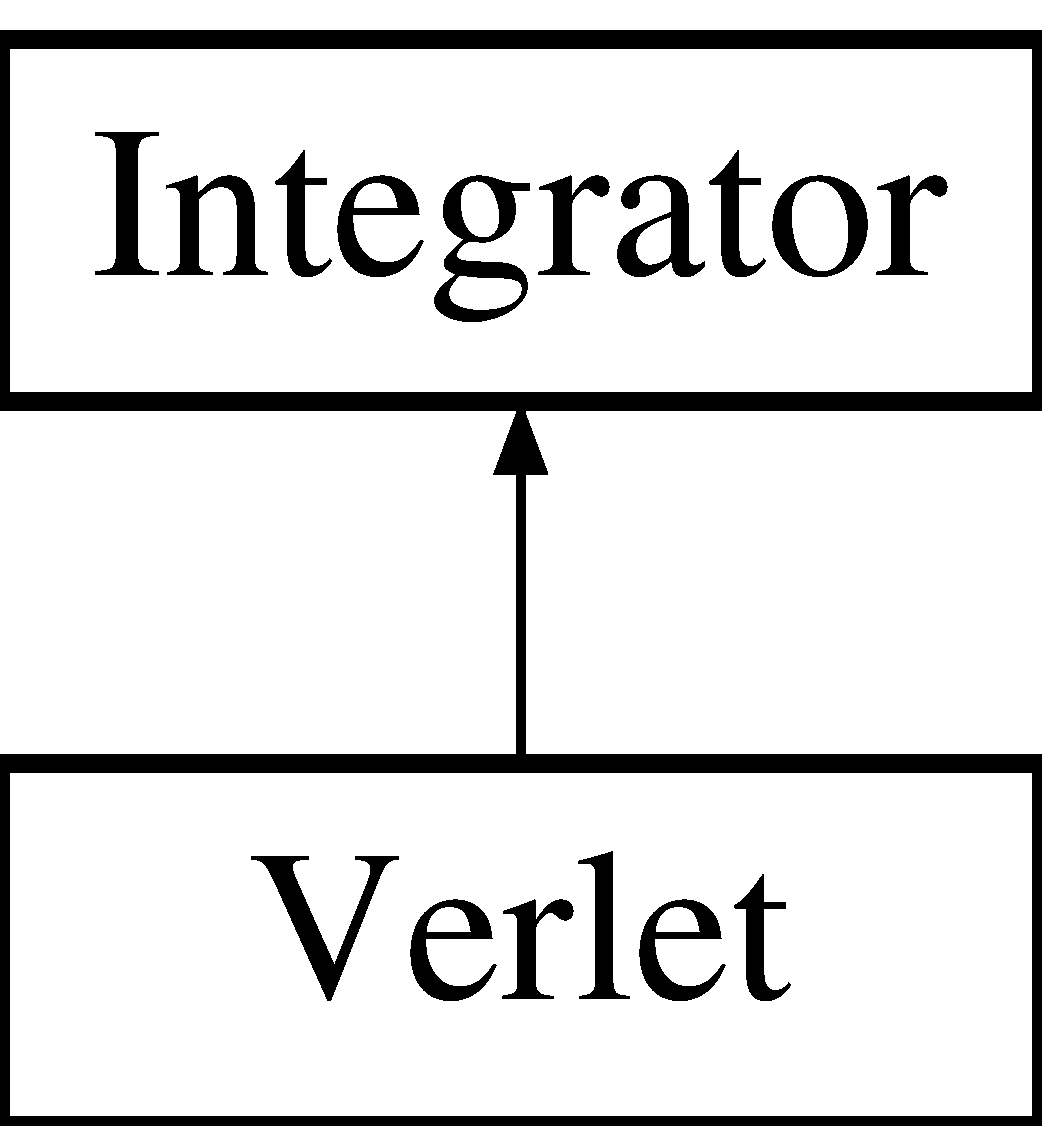
\includegraphics[height=2.000000cm]{classVerlet}
\end{center}
\end{figure}
\subsection*{Public Member Functions}
\begin{DoxyCompactItemize}
\item 
\hyperlink{classVerlet_a73c8d95b91ea71536414d69eadd44542}{Verlet} (double deltat)
\item 
\hypertarget{classVerlet_a69fbd93284e1d588f882831cbde626bc}{double {\bfseries get\-Time} ()}\label{classVerlet_a69fbd93284e1d588f882831cbde626bc}

\item 
\hypertarget{classVerlet_a7cf65ee97242261a681f6fda3901c105}{double {\bfseries getdt} ()}\label{classVerlet_a7cf65ee97242261a681f6fda3901c105}

\item 
int \hyperlink{classVerlet_a1cc9aab24bea5c8c6c1f53ce99582275}{step} (\hyperlink{classSystem}{System} $\ast$sys)
\end{DoxyCompactItemize}
\subsection*{Additional Inherited Members}


\subsection{Detailed Description}
N\-V\-E, \hyperlink{classVerlet}{Verlet}. 

\subsection{Constructor \& Destructor Documentation}
\hypertarget{classVerlet_a73c8d95b91ea71536414d69eadd44542}{\index{Verlet@{Verlet}!Verlet@{Verlet}}
\index{Verlet@{Verlet}!Verlet@{Verlet}}
\subsubsection[{Verlet}]{\setlength{\rightskip}{0pt plus 5cm}Verlet\-::\-Verlet (
\begin{DoxyParamCaption}
\item[{double}]{deltat}
\end{DoxyParamCaption}
)}}\label{classVerlet_a73c8d95b91ea71536414d69eadd44542}

\begin{DoxyParams}[1]{Parameters}
\mbox{\tt in}  & {\em deltat} & Incremental timestep \\
\hline
\end{DoxyParams}


\subsection{Member Function Documentation}
\hypertarget{classVerlet_a1cc9aab24bea5c8c6c1f53ce99582275}{\index{Verlet@{Verlet}!step@{step}}
\index{step@{step}!Verlet@{Verlet}}
\subsubsection[{step}]{\setlength{\rightskip}{0pt plus 5cm}int Verlet\-::step (
\begin{DoxyParamCaption}
\item[{{\bf System} $\ast$}]{sys}
\end{DoxyParamCaption}
)\hspace{0.3cm}{\ttfamily [virtual]}}}\label{classVerlet_a1cc9aab24bea5c8c6c1f53ce99582275}

\begin{DoxyParams}[1]{Parameters}
\mbox{\tt in,out}  & {\em $\ast$sys} & Pointer to \hyperlink{classSystem}{System} to make an integration step in. \\
\hline
\end{DoxyParams}


Implements \hyperlink{classIntegrator_aac53df432f961f8661e157b2a86d8b31}{Integrator}.



The documentation for this class was generated from the following files\-:\begin{DoxyCompactItemize}
\item 
\hyperlink{integrator_8h}{integrator.\-h}\item 
\hyperlink{integrator_8cpp}{integrator.\-cpp}\end{DoxyCompactItemize}

\chapter{File Documentation}
\hypertarget{andersen_8cpp}{\section{andersen.\-cpp File Reference}
\label{andersen_8cpp}\index{andersen.\-cpp@{andersen.\-cpp}}
}


Driver for M\-P\-I Version of C\-B\-E\-M\-D with \hyperlink{classAndersen}{Andersen} Thermostat.  


{\ttfamily \#include \char`\"{}C\-B\-E\-M\-D.\-h\char`\"{}}\\*
\subsection*{Functions}
\begin{DoxyCompactItemize}
\item 
int \hyperlink{andersen_8cpp_a0ddf1224851353fc92bfbff6f499fa97}{main} (int argc, char $\ast$argv\mbox{[}$\,$\mbox{]})
\end{DoxyCompactItemize}


\subsection{Detailed Description}
Driver for M\-P\-I Version of C\-B\-E\-M\-D with \hyperlink{classAndersen}{Andersen} Thermostat. \begin{DoxyAuthor}{Authors}
\{Nathan A. Mahynski, Carmeline Dsilva, Arun L. Prabhu, George Khoury, Frank Ricci, Jun Park\} 
\end{DoxyAuthor}


\subsection{Function Documentation}
\hypertarget{andersen_8cpp_a0ddf1224851353fc92bfbff6f499fa97}{\index{andersen.\-cpp@{andersen.\-cpp}!main@{main}}
\index{main@{main}!andersen.cpp@{andersen.\-cpp}}
\subsubsection[{main}]{\setlength{\rightskip}{0pt plus 5cm}int main (
\begin{DoxyParamCaption}
\item[{int}]{argc, }
\item[{char $\ast$}]{argv\mbox{[}$\,$\mbox{]}}
\end{DoxyParamCaption}
)}}\label{andersen_8cpp_a0ddf1224851353fc92bfbff6f499fa97}

\begin{DoxyParams}{Parameters}
{\em $\ast$argv\mbox{[}$\,$\mbox{]}} & ./andersen nsteps dt temperature xml\-\_\-file bond\-\_\-file animation\-\_\-file temperature nu \\
\hline
\end{DoxyParams}

\hypertarget{atom_8cpp}{\section{atom.\-cpp File Reference}
\label{atom_8cpp}\index{atom.\-cpp@{atom.\-cpp}}
}


Functions for handling M\-D \hyperlink{structAtom}{Atom} Information.  


{\ttfamily \#include \char`\"{}atom.\-h\char`\"{}}\\*
\subsection*{Functions}
\begin{DoxyCompactItemize}
\item 
void \hyperlink{atom_8cpp_ab7a7ac0b58e21d337f3e6face200725d}{create\-\_\-\-M\-P\-I\-\_\-\-A\-T\-O\-M} ()
\begin{DoxyCompactList}\small\item\em Creates the M\-P\-I\-\_\-\-Atom class so it can be passed with M\-P\-I. \end{DoxyCompactList}\item 
void \hyperlink{atom_8cpp_a4b444ef72f56b0f4bb21050ec3fa89da}{delete\-\_\-\-M\-P\-I\-\_\-atom} ()
\begin{DoxyCompactList}\small\item\em Free the M\-P\-I type at the end of the program. \end{DoxyCompactList}\end{DoxyCompactItemize}


\subsection{Detailed Description}
Functions for handling M\-D \hyperlink{structAtom}{Atom} Information. \begin{DoxyAuthor}{Author}
\{Nathan A. Mahynski, Carmeline Dsilva\} 
\end{DoxyAuthor}


\subsection{Function Documentation}
\hypertarget{atom_8cpp_ab7a7ac0b58e21d337f3e6face200725d}{\index{atom.\-cpp@{atom.\-cpp}!create\-\_\-\-M\-P\-I\-\_\-\-A\-T\-O\-M@{create\-\_\-\-M\-P\-I\-\_\-\-A\-T\-O\-M}}
\index{create\-\_\-\-M\-P\-I\-\_\-\-A\-T\-O\-M@{create\-\_\-\-M\-P\-I\-\_\-\-A\-T\-O\-M}!atom.cpp@{atom.\-cpp}}
\subsubsection[{create\-\_\-\-M\-P\-I\-\_\-\-A\-T\-O\-M}]{\setlength{\rightskip}{0pt plus 5cm}void create\-\_\-\-M\-P\-I\-\_\-\-A\-T\-O\-M (
\begin{DoxyParamCaption}
{}
\end{DoxyParamCaption}
)}}\label{atom_8cpp_ab7a7ac0b58e21d337f3e6face200725d}


Creates the M\-P\-I\-\_\-\-Atom class so it can be passed with M\-P\-I. 

This function creates and commits to memory the M\-P\-I\-\_\-\-A\-T\-O\-M derived data type. (see example of use at \href{https://computing.llnl.gov/tutorials/mpi/#Derived_Data_Types}{\tt https\-://computing.\-llnl.\-gov/tutorials/mpi/\#\-Derived\-\_\-\-Data\-\_\-\-Types}) \begin{DoxySeeAlso}{See Also}
initialize, \hyperlink{mpiatom_8h_a628d6a0c02ae3d09415ac91d6c842f23}{M\-P\-I\-\_\-\-A\-T\-O\-M} 
\end{DoxySeeAlso}
\hypertarget{atom_8cpp_a4b444ef72f56b0f4bb21050ec3fa89da}{\index{atom.\-cpp@{atom.\-cpp}!delete\-\_\-\-M\-P\-I\-\_\-atom@{delete\-\_\-\-M\-P\-I\-\_\-atom}}
\index{delete\-\_\-\-M\-P\-I\-\_\-atom@{delete\-\_\-\-M\-P\-I\-\_\-atom}!atom.cpp@{atom.\-cpp}}
\subsubsection[{delete\-\_\-\-M\-P\-I\-\_\-atom}]{\setlength{\rightskip}{0pt plus 5cm}void delete\-\_\-\-M\-P\-I\-\_\-atom (
\begin{DoxyParamCaption}
{}
\end{DoxyParamCaption}
)}}\label{atom_8cpp_a4b444ef72f56b0f4bb21050ec3fa89da}


Free the M\-P\-I type at the end of the program. 

This function utilizes the complementary M\-P\-I\-\_\-\-Type\-\_\-free routine to mark the M\-P\-I\-\_\-\-A\-T\-O\-M type for deallocation at the end of the program. \begin{DoxySeeAlso}{See Also}
finalize 
\end{DoxySeeAlso}

\hypertarget{atom_8h}{\section{atom.\-h File Reference}
\label{atom_8h}\index{atom.\-h@{atom.\-h}}
}


M\-D Atom Information.  


{\ttfamily \#include \char`\"{}common.\-h\char`\"{}}\\*
{\ttfamily \#include \char`\"{}mpi.\-h\char`\"{}}\\*
{\ttfamily \#include \char`\"{}global.\-h\char`\"{}}\\*
\subsection*{Classes}
\begin{DoxyCompactItemize}
\item 
struct \hyperlink{structatom_1_1Atom}{atom\-::\-Atom}
\begin{DoxyCompactList}\small\item\em \hyperlink{structatom_1_1Atom}{Atom} class is defined as a struct so as to be easy to pass with M\-P\-I. \end{DoxyCompactList}\end{DoxyCompactItemize}
\subsection*{Namespaces}
\begin{DoxyCompactItemize}
\item 
namespace \hyperlink{namespaceatom}{atom}
\end{DoxyCompactItemize}
\subsection*{Functions}
\begin{DoxyCompactItemize}
\item 
void \hyperlink{namespaceatom_a2ff83b4e5fd34d597e76d4c0db30db2d}{atom\-::create\-\_\-\-M\-P\-I\-\_\-\-A\-T\-O\-M} ()
\begin{DoxyCompactList}\small\item\em M\-P\-I version of \hyperlink{structatom_1_1Atom}{Atom}. \end{DoxyCompactList}\item 
void \hyperlink{namespaceatom_a810235b68ff377831ea415e440b81a76}{atom\-::delete\-\_\-\-M\-P\-I\-\_\-atom} ()
\begin{DoxyCompactList}\small\item\em Free the M\-P\-I type at the end of the program. \end{DoxyCompactList}\end{DoxyCompactItemize}


\subsection{Detailed Description}
M\-D Atom Information. \begin{DoxyAuthor}{Author}
Nathan A. Mahynski 
\end{DoxyAuthor}

\hypertarget{CBEMD_8h}{\section{C\-B\-E\-M\-D.\-h File Reference}
\label{CBEMD_8h}\index{C\-B\-E\-M\-D.\-h@{C\-B\-E\-M\-D.\-h}}
}


Header grouping source headers into one simple header for the driver program(s).  


{\ttfamily \#include \char`\"{}atom.\-h\char`\"{}}\\*
{\ttfamily \#include \char`\"{}system.\-h\char`\"{}}\\*
{\ttfamily \#include \char`\"{}integrator.\-h\char`\"{}}\\*
{\ttfamily \#include \char`\"{}misc.\-h\char`\"{}}\\*
{\ttfamily \#include \char`\"{}global.\-h\char`\"{}}\\*
{\ttfamily \#include \char`\"{}read\-\_\-xml.\-h\char`\"{}}\\*
{\ttfamily \#include \char`\"{}interaction.\-h\char`\"{}}\\*
{\ttfamily \#include \char`\"{}mpiatom.\-h\char`\"{}}\\*
{\ttfamily \#include \char`\"{}initialize.\-h\char`\"{}}\\*
{\ttfamily \#include \char`\"{}mpi.\-h\char`\"{}}\\*
{\ttfamily \#include $<$limits$>$}\\*


\subsection{Detailed Description}
Header grouping source headers into one simple header for the driver program(s). \begin{DoxyAuthor}{Author}
\{Carmeline Dsilva\} 
\end{DoxyAuthor}

\hypertarget{common_8h}{\section{common.\-h File Reference}
\label{common_8h}\index{common.\-h@{common.\-h}}
}


Header that lumps all common header files into one.  


{\ttfamily \#include $<$iostream$>$}\\*
{\ttfamily \#include $<$cstdio$>$}\\*
{\ttfamily \#include $<$cstdlib$>$}\\*
{\ttfamily \#include $<$cmath$>$}\\*
{\ttfamily \#include $<$vector$>$}\\*
{\ttfamily \#include $<$string$>$}\\*


\subsection{Detailed Description}
Header that lumps all common header files into one. 
\hypertarget{domain__decomp_8cpp}{\section{domain\-\_\-decomp.\-cpp File Reference}
\label{domain__decomp_8cpp}\index{domain\-\_\-decomp.\-cpp@{domain\-\_\-decomp.\-cpp}}
}


Source code containing functions for performing domain decomposition.  


{\ttfamily \#include \char`\"{}domain\-\_\-decomp.\-h\char`\"{}}\\*
\subsection*{Functions}
\begin{DoxyCompactItemize}
\item 
void \hyperlink{domain__decomp_8cpp_a5dff21a3c71bc2b5822508e41fdcf697}{gen\-\_\-sets} (const vector$<$ int $>$ \&factors, const double box\mbox{[}$\,$\mbox{]}, const int level, double \&final\-\_\-diff, vector$<$ int $>$ \&final\-\_\-breakup, int add)
\begin{DoxyCompactList}\small\item\em Given the box size and factors of nprocs, checks which combination generates the most cubic domains. \end{DoxyCompactList}\item 
vector$<$ int $>$ \hyperlink{domain__decomp_8cpp_af08c020490d351043482fe498e7b6f1c}{factorize} (const int nprocs)
\begin{DoxyCompactList}\small\item\em Given a number returns the prime factors (does not count 1 as a prime factor) \end{DoxyCompactList}\item 
int \hyperlink{domain__decomp_8cpp_adb16a776f045b9fd68b06a31ed29c035}{init\-\_\-domain\-\_\-decomp} (const vector$<$ double $>$ box, const int nprocs, double widths\mbox{[}$\,$\mbox{]}, vector$<$ int $>$ \&final\-\_\-breakup)
\begin{DoxyCompactList}\small\item\em Decomposes the box into domains for each processor to handle. \end{DoxyCompactList}\item 
int \hyperlink{domain__decomp_8cpp_ac1a67f8956fb748c46d0d9772a1f6d32}{get\-\_\-processor} (const vector$<$ double $>$ pos, const \hyperlink{classSystem}{System} $\ast$sys)
\begin{DoxyCompactList}\small\item\em Given the co-\/ordinates of a point, determines within which domain the point lies. \end{DoxyCompactList}\item 
int \hyperlink{domain__decomp_8cpp_a233c77efbd17cf4e8b014b90a109c1a1}{get\-\_\-processor} (const int x\-\_\-id, const int y\-\_\-id, const int z\-\_\-id, const vector$<$ int $>$ \&final\-\_\-breakup)
\item 
int \hyperlink{domain__decomp_8cpp_ab7e6998f4d09ce978b0be93256a7aea7}{get\-\_\-xyz\-\_\-ids} (const int domain\-\_\-id, const vector$<$ int $>$ \&final\-\_\-breakup, int xyz\-\_\-id\mbox{[}$\,$\mbox{]})
\begin{DoxyCompactList}\small\item\em Given a domain\-\_\-id specifies the x, y, z ids of the domain. \end{DoxyCompactList}\item 
int \hyperlink{domain__decomp_8cpp_a6089fbe2af876c7807125a3ca60ec325}{gen\-\_\-send\-\_\-lists} (\hyperlink{classSystem}{System} $\ast$sys)
\begin{DoxyCompactList}\small\item\em Generates the lists of molecules that need to be passed to other processors. \end{DoxyCompactList}\item 
int \hyperlink{domain__decomp_8cpp_a91bec4369dfa716b9da0f3768b42f0b6}{gen\-\_\-send\-\_\-table} (\hyperlink{classSystem}{System} $\ast$sys)
\begin{DoxyCompactList}\small\item\em Given the rank, generates the list of its neighbours. \end{DoxyCompactList}\item 
void \hyperlink{domain__decomp_8cpp_a273ef862952335fba02a34fbf164180c}{gen\-\_\-goes\-\_\-to} (const vector$<$ int $>$ \&is\-\_\-near\-\_\-border, vector$<$ int $>$ \&goes\-\_\-to, const int ndims)
\begin{DoxyCompactList}\small\item\em Generates the list of neighbours a particle should be sent to based on the borders its near. \end{DoxyCompactList}\item 
int \hyperlink{domain__decomp_8cpp_aee4072f52ae76435a626b818498e3e27}{power} (int base, int exponent)
\begin{DoxyCompactList}\small\item\em Computes the exponentiation of an integer by an integral power. \end{DoxyCompactList}\item 
int \hyperlink{domain__decomp_8cpp_a66b4457a4c1558782b561737fccb1f39}{communicate\-\_\-skin\-\_\-atoms} (\hyperlink{classSystem}{System} $\ast$sys)
\begin{DoxyCompactList}\small\item\em Communicates the atoms in the skin regions of the processors to the appropriate neighbours. \end{DoxyCompactList}\end{DoxyCompactItemize}


\subsection{Detailed Description}
Source code containing functions for performing domain decomposition. \begin{DoxyAuthor}{Author}
Arun L. Prabhu 
\end{DoxyAuthor}


\subsection{Function Documentation}
\hypertarget{domain__decomp_8cpp_a66b4457a4c1558782b561737fccb1f39}{\index{domain\-\_\-decomp.\-cpp@{domain\-\_\-decomp.\-cpp}!communicate\-\_\-skin\-\_\-atoms@{communicate\-\_\-skin\-\_\-atoms}}
\index{communicate\-\_\-skin\-\_\-atoms@{communicate\-\_\-skin\-\_\-atoms}!domain_decomp.cpp@{domain\-\_\-decomp.\-cpp}}
\subsubsection[{communicate\-\_\-skin\-\_\-atoms}]{\setlength{\rightskip}{0pt plus 5cm}int communicate\-\_\-skin\-\_\-atoms (
\begin{DoxyParamCaption}
\item[{{\bf System} $\ast$}]{sys}
\end{DoxyParamCaption}
)}}\label{domain__decomp_8cpp_a66b4457a4c1558782b561737fccb1f39}


Communicates the atoms in the skin regions of the processors to the appropriate neighbours. 

Communicates the atoms in the skin regions of the processors to the appropriate neighbours 
\begin{DoxyParams}{Parameters}
{\em sys} & \mbox{[}in,out\mbox{]} \hyperlink{classSystem}{System} to be evaluated \\
\hline
\end{DoxyParams}
\hypertarget{domain__decomp_8cpp_af08c020490d351043482fe498e7b6f1c}{\index{domain\-\_\-decomp.\-cpp@{domain\-\_\-decomp.\-cpp}!factorize@{factorize}}
\index{factorize@{factorize}!domain_decomp.cpp@{domain\-\_\-decomp.\-cpp}}
\subsubsection[{factorize}]{\setlength{\rightskip}{0pt plus 5cm}vector$<$int$>$ factorize (
\begin{DoxyParamCaption}
\item[{const int}]{nprocs}
\end{DoxyParamCaption}
)}}\label{domain__decomp_8cpp_af08c020490d351043482fe498e7b6f1c}


Given a number returns the prime factors (does not count 1 as a prime factor) 

Given a number returns the prime factors of that number. This function does not count 1 as a prime factor. 
\begin{DoxyParams}[1]{Parameters}
\mbox{\tt in}  & {\em nprocs} & number of processors \\
\hline
\end{DoxyParams}
\hypertarget{domain__decomp_8cpp_a273ef862952335fba02a34fbf164180c}{\index{domain\-\_\-decomp.\-cpp@{domain\-\_\-decomp.\-cpp}!gen\-\_\-goes\-\_\-to@{gen\-\_\-goes\-\_\-to}}
\index{gen\-\_\-goes\-\_\-to@{gen\-\_\-goes\-\_\-to}!domain_decomp.cpp@{domain\-\_\-decomp.\-cpp}}
\subsubsection[{gen\-\_\-goes\-\_\-to}]{\setlength{\rightskip}{0pt plus 5cm}void gen\-\_\-goes\-\_\-to (
\begin{DoxyParamCaption}
\item[{const vector$<$ int $>$ \&}]{is\-\_\-near\-\_\-border, }
\item[{vector$<$ int $>$ \&}]{goes\-\_\-to, }
\item[{const int}]{ndims}
\end{DoxyParamCaption}
)}}\label{domain__decomp_8cpp_a273ef862952335fba02a34fbf164180c}


Generates the list of neighbours a particle should be sent to based on the borders its near. 

Generates the list of neighbours a particle should be sent to based on the borders its near 
\begin{DoxyParams}[1]{Parameters}
\mbox{\tt in}  & {\em is\-\_\-near\-\_\-border} & information about which borders an atom is near \\
\hline
 & {\em goes\-\_\-to} & \mbox{[}in\mbox{]} vector containing the ids the current atoms needs to be communicated to \\
\hline
\mbox{\tt in}  & {\em ndims} & the number of dimensions of the simulation \\
\hline
\end{DoxyParams}
\hypertarget{domain__decomp_8cpp_a6089fbe2af876c7807125a3ca60ec325}{\index{domain\-\_\-decomp.\-cpp@{domain\-\_\-decomp.\-cpp}!gen\-\_\-send\-\_\-lists@{gen\-\_\-send\-\_\-lists}}
\index{gen\-\_\-send\-\_\-lists@{gen\-\_\-send\-\_\-lists}!domain_decomp.cpp@{domain\-\_\-decomp.\-cpp}}
\subsubsection[{gen\-\_\-send\-\_\-lists}]{\setlength{\rightskip}{0pt plus 5cm}int gen\-\_\-send\-\_\-lists (
\begin{DoxyParamCaption}
\item[{{\bf System} $\ast$}]{sys}
\end{DoxyParamCaption}
)}}\label{domain__decomp_8cpp_a6089fbe2af876c7807125a3ca60ec325}


Generates the lists of molecules that need to be passed to other processors. 

Generates the lists of molecules that need to be passed to other processors 
\begin{DoxyParams}[1]{Parameters}
\mbox{\tt in,out}  & {\em sys} & \hyperlink{classSystem}{System} to be evaluated \\
\hline
\end{DoxyParams}
\hypertarget{domain__decomp_8cpp_a91bec4369dfa716b9da0f3768b42f0b6}{\index{domain\-\_\-decomp.\-cpp@{domain\-\_\-decomp.\-cpp}!gen\-\_\-send\-\_\-table@{gen\-\_\-send\-\_\-table}}
\index{gen\-\_\-send\-\_\-table@{gen\-\_\-send\-\_\-table}!domain_decomp.cpp@{domain\-\_\-decomp.\-cpp}}
\subsubsection[{gen\-\_\-send\-\_\-table}]{\setlength{\rightskip}{0pt plus 5cm}int gen\-\_\-send\-\_\-table (
\begin{DoxyParamCaption}
\item[{{\bf System} $\ast$}]{sys}
\end{DoxyParamCaption}
)}}\label{domain__decomp_8cpp_a91bec4369dfa716b9da0f3768b42f0b6}


Given the rank, generates the list of its neighbours. 

Given the rank, generates the list of its neighbours Assumes 3\-D system, for different number of dimensions need to make this a recursive function 
\begin{DoxyParams}[1]{Parameters}
\mbox{\tt in,out}  & {\em sys} & \hyperlink{classSystem}{System} to be evaluated \\
\hline
\end{DoxyParams}
\hypertarget{domain__decomp_8cpp_a5dff21a3c71bc2b5822508e41fdcf697}{\index{domain\-\_\-decomp.\-cpp@{domain\-\_\-decomp.\-cpp}!gen\-\_\-sets@{gen\-\_\-sets}}
\index{gen\-\_\-sets@{gen\-\_\-sets}!domain_decomp.cpp@{domain\-\_\-decomp.\-cpp}}
\subsubsection[{gen\-\_\-sets}]{\setlength{\rightskip}{0pt plus 5cm}void gen\-\_\-sets (
\begin{DoxyParamCaption}
\item[{const vector$<$ int $>$ \&}]{factors, }
\item[{const double}]{box\mbox{[}$\,$\mbox{]}, }
\item[{const int}]{level, }
\item[{double \&}]{final\-\_\-diff, }
\item[{vector$<$ int $>$ \&}]{final\-\_\-breakup, }
\item[{int}]{add}
\end{DoxyParamCaption}
)}}\label{domain__decomp_8cpp_a5dff21a3c71bc2b5822508e41fdcf697}


Given the box size and factors of nprocs, checks which combination generates the most cubic domains. 

Given the box size and factors of nprocs, this recursive function checks which combination generates the most cubic domains 
\begin{DoxyParams}[1]{Parameters}
\mbox{\tt in}  & {\em factors} & list of prime factors to be used \\
\hline
\mbox{\tt in}  & {\em box} & dimensions of the simulation box \\
\hline
\mbox{\tt in}  & {\em level} & the depth of the recursion \\
\hline
\mbox{\tt out}  & {\em final\-\_\-breakup} & the number of divisions of each dimension \\
\hline
\mbox{\tt in}  & {\em add} & the number of times to be spent at this level of recursion \\
\hline
\end{DoxyParams}
\hypertarget{domain__decomp_8cpp_ac1a67f8956fb748c46d0d9772a1f6d32}{\index{domain\-\_\-decomp.\-cpp@{domain\-\_\-decomp.\-cpp}!get\-\_\-processor@{get\-\_\-processor}}
\index{get\-\_\-processor@{get\-\_\-processor}!domain_decomp.cpp@{domain\-\_\-decomp.\-cpp}}
\subsubsection[{get\-\_\-processor}]{\setlength{\rightskip}{0pt plus 5cm}int get\-\_\-processor (
\begin{DoxyParamCaption}
\item[{const vector$<$ double $>$}]{pos, }
\item[{const {\bf System} $\ast$}]{sys}
\end{DoxyParamCaption}
)}}\label{domain__decomp_8cpp_ac1a67f8956fb748c46d0d9772a1f6d32}


Given the co-\/ordinates of a point, determines within which domain the point lies. 

Given the coordinates of a point, determines within which domain the point lies. This function is overloaded. 
\begin{DoxyParams}[1]{Parameters}
\mbox{\tt in}  & {\em pos} & the vector containing the coordinates of a point \\
\hline
\mbox{\tt in}  & {\em sys} & system passed to be able to utilize final domain decomposition \\
\hline
\end{DoxyParams}
\hypertarget{domain__decomp_8cpp_a233c77efbd17cf4e8b014b90a109c1a1}{\index{domain\-\_\-decomp.\-cpp@{domain\-\_\-decomp.\-cpp}!get\-\_\-processor@{get\-\_\-processor}}
\index{get\-\_\-processor@{get\-\_\-processor}!domain_decomp.cpp@{domain\-\_\-decomp.\-cpp}}
\subsubsection[{get\-\_\-processor}]{\setlength{\rightskip}{0pt plus 5cm}int get\-\_\-processor (
\begin{DoxyParamCaption}
\item[{const int}]{x\-\_\-id, }
\item[{const int}]{y\-\_\-id, }
\item[{const int}]{z\-\_\-id, }
\item[{const vector$<$ int $>$ \&}]{final\-\_\-breakup}
\end{DoxyParamCaption}
)}}\label{domain__decomp_8cpp_a233c77efbd17cf4e8b014b90a109c1a1}
Given the coordinates of a point, determines within which domain the point lies. This function is overloaded. 
\begin{DoxyParams}[1]{Parameters}
\mbox{\tt in}  & {\em x\-\_\-id} & how many domains away from x\-\_\-min the current domain is \\
\hline
\mbox{\tt in}  & {\em y\-\_\-id} & how many domains away from y\-\_\-min the current domain is \\
\hline
\mbox{\tt in}  & {\em z\-\_\-id} & how many domains away from z\-\_\-min the current domain is \\
\hline
\mbox{\tt in}  & {\em fina\-\_\-breakup} & the number of divisions of each dimension \\
\hline
\end{DoxyParams}
\hypertarget{domain__decomp_8cpp_ab7e6998f4d09ce978b0be93256a7aea7}{\index{domain\-\_\-decomp.\-cpp@{domain\-\_\-decomp.\-cpp}!get\-\_\-xyz\-\_\-ids@{get\-\_\-xyz\-\_\-ids}}
\index{get\-\_\-xyz\-\_\-ids@{get\-\_\-xyz\-\_\-ids}!domain_decomp.cpp@{domain\-\_\-decomp.\-cpp}}
\subsubsection[{get\-\_\-xyz\-\_\-ids}]{\setlength{\rightskip}{0pt plus 5cm}int get\-\_\-xyz\-\_\-ids (
\begin{DoxyParamCaption}
\item[{const int}]{domain\-\_\-id, }
\item[{const vector$<$ int $>$ \&}]{final\-\_\-breakup, }
\item[{int}]{xyz\-\_\-id\mbox{[}$\,$\mbox{]}}
\end{DoxyParamCaption}
)}}\label{domain__decomp_8cpp_ab7e6998f4d09ce978b0be93256a7aea7}


Given a domain\-\_\-id specifies the x, y, z ids of the domain. 

Given a domain\-\_\-id specifies the x, y, z ids of the domain 
\begin{DoxyParams}[1]{Parameters}
\mbox{\tt in}  & {\em domain\-\_\-id} & domain identifier, same as the rank of the processor handling the domain \\
\hline
\mbox{\tt in}  & {\em final\-\_\-breakup} & the number of divisions of each dimension \\
\hline
\mbox{\tt in}  & {\em xyz\-\_\-id} & how many domains away from the lower limit of each dimension the current domain is \\
\hline
\end{DoxyParams}
\hypertarget{domain__decomp_8cpp_adb16a776f045b9fd68b06a31ed29c035}{\index{domain\-\_\-decomp.\-cpp@{domain\-\_\-decomp.\-cpp}!init\-\_\-domain\-\_\-decomp@{init\-\_\-domain\-\_\-decomp}}
\index{init\-\_\-domain\-\_\-decomp@{init\-\_\-domain\-\_\-decomp}!domain_decomp.cpp@{domain\-\_\-decomp.\-cpp}}
\subsubsection[{init\-\_\-domain\-\_\-decomp}]{\setlength{\rightskip}{0pt plus 5cm}int init\-\_\-domain\-\_\-decomp (
\begin{DoxyParamCaption}
\item[{const vector$<$ double $>$}]{box, }
\item[{const int}]{nprocs, }
\item[{double}]{widths\mbox{[}$\,$\mbox{]}, }
\item[{vector$<$ int $>$ \&}]{final\-\_\-breakup}
\end{DoxyParamCaption}
)}}\label{domain__decomp_8cpp_adb16a776f045b9fd68b06a31ed29c035}


Decomposes the box into domains for each processor to handle. 

Decomposes the box into domains for each processor to handle 
\begin{DoxyParams}[1]{Parameters}
\mbox{\tt in}  & {\em box} & dimensions of the simulation box \\
\hline
\mbox{\tt in}  & {\em nprocs} & number of processors \\
\hline
\mbox{\tt in}  & {\em widths} & the dimensions of each domain \\
\hline
\mbox{\tt out}  & {\em final\-\_\-breakup} & the number of divisions of each dimension \\
\hline
\end{DoxyParams}
\hypertarget{domain__decomp_8cpp_aee4072f52ae76435a626b818498e3e27}{\index{domain\-\_\-decomp.\-cpp@{domain\-\_\-decomp.\-cpp}!power@{power}}
\index{power@{power}!domain_decomp.cpp@{domain\-\_\-decomp.\-cpp}}
\subsubsection[{power}]{\setlength{\rightskip}{0pt plus 5cm}int power (
\begin{DoxyParamCaption}
\item[{int}]{base, }
\item[{int}]{exponent}
\end{DoxyParamCaption}
)}}\label{domain__decomp_8cpp_aee4072f52ae76435a626b818498e3e27}


Computes the exponentiation of an integer by an integral power. 

Computes the exponentiation of an integer by an integral power 
\begin{DoxyParams}[1]{Parameters}
\mbox{\tt in}  & {\em base} & the base value to be raised to a power \\
\hline
\mbox{\tt in}  & {\em exponent} & the exponent of the power base is raised to \\
\hline
\end{DoxyParams}

\hypertarget{domain__decomp_8h}{\section{domain\-\_\-decomp.\-h File Reference}
\label{domain__decomp_8h}\index{domain\-\_\-decomp.\-h@{domain\-\_\-decomp.\-h}}
}


Header file for domain decomposition.  


{\ttfamily \#include \char`\"{}common.\-h\char`\"{}}\\*
{\ttfamily \#include \char`\"{}system.\-h\char`\"{}}\\*
{\ttfamily \#include \char`\"{}mpi.\-h\char`\"{}}\\*
\subsection*{Functions}
\begin{DoxyCompactItemize}
\item 
void \hyperlink{domain__decomp_8h_a5dff21a3c71bc2b5822508e41fdcf697}{gen\-\_\-sets} (const vector$<$ int $>$ \&factors, const double box\mbox{[}$\,$\mbox{]}, const int level, double \&final\-\_\-diff, vector$<$ int $>$ \&final\-\_\-breakup, int add)
\begin{DoxyCompactList}\small\item\em Given the box size and factors of nprocs, checks which combination generates the most cubic domains. \end{DoxyCompactList}\item 
vector$<$ int $>$ \hyperlink{domain__decomp_8h_af08c020490d351043482fe498e7b6f1c}{factorize} (const int nprocs)
\begin{DoxyCompactList}\small\item\em Given a number returns the prime factors (does not count 1 as a prime factor) \end{DoxyCompactList}\item 
int \hyperlink{domain__decomp_8h_adb16a776f045b9fd68b06a31ed29c035}{init\-\_\-domain\-\_\-decomp} (const vector$<$ double $>$ box, const int nprocs, double widths\mbox{[}$\,$\mbox{]}, vector$<$ int $>$ \&final\-\_\-breakup)
\begin{DoxyCompactList}\small\item\em Decomposes the box into domains for each processor to handle. \end{DoxyCompactList}\item 
int \hyperlink{domain__decomp_8h_ac1a67f8956fb748c46d0d9772a1f6d32}{get\-\_\-processor} (const vector$<$ double $>$ pos, const \hyperlink{classsim__system_1_1System}{System} $\ast$sys)
\begin{DoxyCompactList}\small\item\em Given the co-\/ordinates of a point, determines within which domain the point lies. \end{DoxyCompactList}\item 
\hypertarget{domain__decomp_8h_ab4a446734f29c8476be0c8766871205a}{int \hyperlink{domain__decomp_8h_ab4a446734f29c8476be0c8766871205a}{get\-\_\-processor\-\_\-id} (const int x\-\_\-id, const int y\-\_\-id, const int z\-\_\-id, const vector$<$ int $>$ \&final\-\_\-breakup)}\label{domain__decomp_8h_ab4a446734f29c8476be0c8766871205a}

\begin{DoxyCompactList}\small\item\em Given the x, y, z ids of a domain, determines the domain id (useful for locating neighbouring domains) \end{DoxyCompactList}\item 
int \hyperlink{domain__decomp_8h_ab7e6998f4d09ce978b0be93256a7aea7}{get\-\_\-xyz\-\_\-ids} (const int domain\-\_\-id, const vector$<$ int $>$ \&final\-\_\-breakup, int xyz\-\_\-id\mbox{[}$\,$\mbox{]})
\begin{DoxyCompactList}\small\item\em Given a domain\-\_\-id specifies the x, y, z ids of the domain. \end{DoxyCompactList}\item 
int \hyperlink{domain__decomp_8h_a6089fbe2af876c7807125a3ca60ec325}{gen\-\_\-send\-\_\-lists} (\hyperlink{classsim__system_1_1System}{System} $\ast$sys)
\begin{DoxyCompactList}\small\item\em Generates the lists of molecules that need to be passed to other processors. \end{DoxyCompactList}\item 
int \hyperlink{domain__decomp_8h_a91bec4369dfa716b9da0f3768b42f0b6}{gen\-\_\-send\-\_\-table} (\hyperlink{classsim__system_1_1System}{System} $\ast$sys)
\begin{DoxyCompactList}\small\item\em Given the rank, generates the list of its neighbours. \end{DoxyCompactList}\item 
\hypertarget{domain__decomp_8h_a310ac8170d9320c54906bed20e391478}{double \hyperlink{domain__decomp_8h_a310ac8170d9320c54906bed20e391478}{gen\-\_\-skin\-\_\-cutoff} (...)}\label{domain__decomp_8h_a310ac8170d9320c54906bed20e391478}

\begin{DoxyCompactList}\small\item\em Generates the skin cutoff distance based on the largest cutoff in the system. \end{DoxyCompactList}\item 
void \hyperlink{domain__decomp_8h_a273ef862952335fba02a34fbf164180c}{gen\-\_\-goes\-\_\-to} (const vector$<$ int $>$ \&is\-\_\-near\-\_\-border, vector$<$ int $>$ \&goes\-\_\-to, const int ndims)
\begin{DoxyCompactList}\small\item\em Generates the list of neighbours a particle should be sent to based on the borders its near. \end{DoxyCompactList}\item 
int \hyperlink{domain__decomp_8h_aee4072f52ae76435a626b818498e3e27}{power} (int base, int exponent)
\begin{DoxyCompactList}\small\item\em Computes the exponentiation of an integer by an integral power. \end{DoxyCompactList}\item 
int \hyperlink{domain__decomp_8h_a66b4457a4c1558782b561737fccb1f39}{communicate\-\_\-skin\-\_\-atoms} (\hyperlink{classsim__system_1_1System}{System} $\ast$sys)
\begin{DoxyCompactList}\small\item\em Communicates the atoms in the skin regions of the processors to the appropriate neighbours. \end{DoxyCompactList}\end{DoxyCompactItemize}


\subsection{Detailed Description}
Header file for domain decomposition. \begin{DoxyAuthor}{Author}
Arun L. Prabhu 
\end{DoxyAuthor}


\subsection{Function Documentation}
\hypertarget{domain__decomp_8h_a66b4457a4c1558782b561737fccb1f39}{\index{domain\-\_\-decomp.\-h@{domain\-\_\-decomp.\-h}!communicate\-\_\-skin\-\_\-atoms@{communicate\-\_\-skin\-\_\-atoms}}
\index{communicate\-\_\-skin\-\_\-atoms@{communicate\-\_\-skin\-\_\-atoms}!domain_decomp.h@{domain\-\_\-decomp.\-h}}
\subsubsection[{communicate\-\_\-skin\-\_\-atoms}]{\setlength{\rightskip}{0pt plus 5cm}int communicate\-\_\-skin\-\_\-atoms (
\begin{DoxyParamCaption}
\item[{{\bf System} $\ast$}]{sys}
\end{DoxyParamCaption}
)}}\label{domain__decomp_8h_a66b4457a4c1558782b561737fccb1f39}


Communicates the atoms in the skin regions of the processors to the appropriate neighbours. 

Communicates the atoms in the skin regions of the processors to the appropriate neighbours 
\begin{DoxyParams}{Parameters}
{\em sys} & \mbox{[}in,out\mbox{]} System to be evaluated \\
\hline
\end{DoxyParams}
\hypertarget{domain__decomp_8h_af08c020490d351043482fe498e7b6f1c}{\index{domain\-\_\-decomp.\-h@{domain\-\_\-decomp.\-h}!factorize@{factorize}}
\index{factorize@{factorize}!domain_decomp.h@{domain\-\_\-decomp.\-h}}
\subsubsection[{factorize}]{\setlength{\rightskip}{0pt plus 5cm}vector$<$int$>$ factorize (
\begin{DoxyParamCaption}
\item[{const int}]{nprocs}
\end{DoxyParamCaption}
)}}\label{domain__decomp_8h_af08c020490d351043482fe498e7b6f1c}


Given a number returns the prime factors (does not count 1 as a prime factor) 

Given a number returns the prime factors of that number. This function does not count 1 as a prime factor. 
\begin{DoxyParams}[1]{Parameters}
\mbox{\tt in}  & {\em nprocs} & number of processors \\
\hline
\end{DoxyParams}
\hypertarget{domain__decomp_8h_a273ef862952335fba02a34fbf164180c}{\index{domain\-\_\-decomp.\-h@{domain\-\_\-decomp.\-h}!gen\-\_\-goes\-\_\-to@{gen\-\_\-goes\-\_\-to}}
\index{gen\-\_\-goes\-\_\-to@{gen\-\_\-goes\-\_\-to}!domain_decomp.h@{domain\-\_\-decomp.\-h}}
\subsubsection[{gen\-\_\-goes\-\_\-to}]{\setlength{\rightskip}{0pt plus 5cm}void gen\-\_\-goes\-\_\-to (
\begin{DoxyParamCaption}
\item[{const vector$<$ int $>$ \&}]{is\-\_\-near\-\_\-border, }
\item[{vector$<$ int $>$ \&}]{goes\-\_\-to, }
\item[{const int}]{ndims}
\end{DoxyParamCaption}
)}}\label{domain__decomp_8h_a273ef862952335fba02a34fbf164180c}


Generates the list of neighbours a particle should be sent to based on the borders its near. 

Generates the list of neighbours a particle should be sent to based on the borders its near 
\begin{DoxyParams}[1]{Parameters}
\mbox{\tt in}  & {\em is\-\_\-near\-\_\-border} & W\-H\-A\-T D\-O\-E\-S I\-T D\-O \\
\hline
 & {\em goes\-\_\-to} & \mbox{[}in\mbox{]} W\-H\-A\-T D\-O\-E\-S I\-T D\-O \\
\hline
\mbox{\tt in}  & {\em ndims} & W\-H\-A\-T D\-O\-E\-S I\-T D\-O \\
\hline
\end{DoxyParams}
\hypertarget{domain__decomp_8h_a6089fbe2af876c7807125a3ca60ec325}{\index{domain\-\_\-decomp.\-h@{domain\-\_\-decomp.\-h}!gen\-\_\-send\-\_\-lists@{gen\-\_\-send\-\_\-lists}}
\index{gen\-\_\-send\-\_\-lists@{gen\-\_\-send\-\_\-lists}!domain_decomp.h@{domain\-\_\-decomp.\-h}}
\subsubsection[{gen\-\_\-send\-\_\-lists}]{\setlength{\rightskip}{0pt plus 5cm}int gen\-\_\-send\-\_\-lists (
\begin{DoxyParamCaption}
\item[{{\bf System} $\ast$}]{sys}
\end{DoxyParamCaption}
)}}\label{domain__decomp_8h_a6089fbe2af876c7807125a3ca60ec325}


Generates the lists of molecules that need to be passed to other processors. 

Generates the lists of molecules that need to be passed to other processors 
\begin{DoxyParams}[1]{Parameters}
\mbox{\tt in,out}  & {\em sys} & W\-H\-A\-T D\-O\-E\-S I\-T D\-O \\
\hline
\mbox{\tt in}  & {\em rank} & rank of processor \\
\hline
\mbox{\tt in}  & {\em skin\-\_\-cutoff} & W\-H\-A\-T D\-O\-E\-S I\-T D\-O \\
\hline
\end{DoxyParams}
\hypertarget{domain__decomp_8h_a91bec4369dfa716b9da0f3768b42f0b6}{\index{domain\-\_\-decomp.\-h@{domain\-\_\-decomp.\-h}!gen\-\_\-send\-\_\-table@{gen\-\_\-send\-\_\-table}}
\index{gen\-\_\-send\-\_\-table@{gen\-\_\-send\-\_\-table}!domain_decomp.h@{domain\-\_\-decomp.\-h}}
\subsubsection[{gen\-\_\-send\-\_\-table}]{\setlength{\rightskip}{0pt plus 5cm}int gen\-\_\-send\-\_\-table (
\begin{DoxyParamCaption}
\item[{{\bf System} $\ast$}]{sys}
\end{DoxyParamCaption}
)}}\label{domain__decomp_8h_a91bec4369dfa716b9da0f3768b42f0b6}


Given the rank, generates the list of its neighbours. 

Given the rank, generates the list of its neighbours Assumes 3\-D system, for different number of dimensions need to make this a recursive function 
\begin{DoxyParams}[1]{Parameters}
\mbox{\tt in}  & {\em sys} & W\-H\-A\-T D\-O\-E\-S I\-T D\-O \\
\hline
\end{DoxyParams}
\hypertarget{domain__decomp_8h_a5dff21a3c71bc2b5822508e41fdcf697}{\index{domain\-\_\-decomp.\-h@{domain\-\_\-decomp.\-h}!gen\-\_\-sets@{gen\-\_\-sets}}
\index{gen\-\_\-sets@{gen\-\_\-sets}!domain_decomp.h@{domain\-\_\-decomp.\-h}}
\subsubsection[{gen\-\_\-sets}]{\setlength{\rightskip}{0pt plus 5cm}void gen\-\_\-sets (
\begin{DoxyParamCaption}
\item[{const vector$<$ int $>$ \&}]{factors, }
\item[{const double}]{box\mbox{[}$\,$\mbox{]}, }
\item[{const int}]{level, }
\item[{double \&}]{final\-\_\-diff, }
\item[{vector$<$ int $>$ \&}]{final\-\_\-breakup, }
\item[{int}]{add}
\end{DoxyParamCaption}
)}}\label{domain__decomp_8h_a5dff21a3c71bc2b5822508e41fdcf697}


Given the box size and factors of nprocs, checks which combination generates the most cubic domains. 

Given the box size and factors of nprocs, this recursive function checks which combination generates the most cubic domains 
\begin{DoxyParams}[1]{Parameters}
\mbox{\tt in}  & {\em factors} & W\-H\-A\-T D\-O\-E\-S I\-T D\-O \\
\hline
\mbox{\tt in}  & {\em box} & W\-H\-A\-T D\-O\-E\-S I\-T D\-O \\
\hline
\mbox{\tt in}  & {\em level} & W\-H\-A\-T D\-O\-E\-S I\-T D\-O \\
\hline
\mbox{\tt in}  & {\em final\-\_\-breakup} & W\-H\-A\-T D\-O\-E\-S I\-T D\-O \\
\hline
\end{DoxyParams}
\hypertarget{domain__decomp_8h_ac1a67f8956fb748c46d0d9772a1f6d32}{\index{domain\-\_\-decomp.\-h@{domain\-\_\-decomp.\-h}!get\-\_\-processor@{get\-\_\-processor}}
\index{get\-\_\-processor@{get\-\_\-processor}!domain_decomp.h@{domain\-\_\-decomp.\-h}}
\subsubsection[{get\-\_\-processor}]{\setlength{\rightskip}{0pt plus 5cm}int get\-\_\-processor (
\begin{DoxyParamCaption}
\item[{const vector$<$ double $>$}]{pos, }
\item[{const {\bf System} $\ast$}]{sys}
\end{DoxyParamCaption}
)}}\label{domain__decomp_8h_ac1a67f8956fb748c46d0d9772a1f6d32}


Given the co-\/ordinates of a point, determines within which domain the point lies. 

Given the coordinates of a point, determines within which domain the point lies. This function is overloaded. 
\begin{DoxyParams}[1]{Parameters}
\mbox{\tt in}  & {\em pos} & the vector containing the coordinates of a point \\
\hline
\mbox{\tt in}  & {\em sys} & system passed to be able to utilize final domain decomposition \\
\hline
\end{DoxyParams}
\hypertarget{domain__decomp_8h_ab7e6998f4d09ce978b0be93256a7aea7}{\index{domain\-\_\-decomp.\-h@{domain\-\_\-decomp.\-h}!get\-\_\-xyz\-\_\-ids@{get\-\_\-xyz\-\_\-ids}}
\index{get\-\_\-xyz\-\_\-ids@{get\-\_\-xyz\-\_\-ids}!domain_decomp.h@{domain\-\_\-decomp.\-h}}
\subsubsection[{get\-\_\-xyz\-\_\-ids}]{\setlength{\rightskip}{0pt plus 5cm}int get\-\_\-xyz\-\_\-ids (
\begin{DoxyParamCaption}
\item[{const int}]{domain\-\_\-id, }
\item[{const vector$<$ int $>$ \&}]{final\-\_\-breakup, }
\item[{int}]{xyz\-\_\-id\mbox{[}$\,$\mbox{]}}
\end{DoxyParamCaption}
)}}\label{domain__decomp_8h_ab7e6998f4d09ce978b0be93256a7aea7}


Given a domain\-\_\-id specifies the x, y, z ids of the domain. 

Given a domain\-\_\-id specifies the x, y, z ids of the domain 
\begin{DoxyParams}[1]{Parameters}
\mbox{\tt in}  & {\em domain\-\_\-id} & W\-H\-A\-T D\-O\-E\-S I\-T D\-O \\
\hline
\mbox{\tt in}  & {\em final\-\_\-breakup} & W\-H\-A\-T D\-O\-E\-S I\-T D\-O \\
\hline
\mbox{\tt in}  & {\em xyz\-\_\-id} & W\-H\-A\-T D\-O\-E\-S I\-T D\-O \\
\hline
\end{DoxyParams}
\hypertarget{domain__decomp_8h_adb16a776f045b9fd68b06a31ed29c035}{\index{domain\-\_\-decomp.\-h@{domain\-\_\-decomp.\-h}!init\-\_\-domain\-\_\-decomp@{init\-\_\-domain\-\_\-decomp}}
\index{init\-\_\-domain\-\_\-decomp@{init\-\_\-domain\-\_\-decomp}!domain_decomp.h@{domain\-\_\-decomp.\-h}}
\subsubsection[{init\-\_\-domain\-\_\-decomp}]{\setlength{\rightskip}{0pt plus 5cm}int init\-\_\-domain\-\_\-decomp (
\begin{DoxyParamCaption}
\item[{const vector$<$ double $>$}]{box, }
\item[{const int}]{nprocs, }
\item[{double}]{widths\mbox{[}$\,$\mbox{]}, }
\item[{vector$<$ int $>$ \&}]{final\-\_\-breakup}
\end{DoxyParamCaption}
)}}\label{domain__decomp_8h_adb16a776f045b9fd68b06a31ed29c035}


Decomposes the box into domains for each processor to handle. 

Decomposes the box into domains for each processor to handle 
\begin{DoxyParams}[1]{Parameters}
\mbox{\tt in}  & {\em box} & W\-H\-A\-T D\-O\-E\-S I\-T D\-O \\
\hline
\mbox{\tt in}  & {\em nprocs} & number of processors \\
\hline
\mbox{\tt in}  & {\em widths} & W\-H\-A\-T D\-O\-E\-S I\-T D\-O \\
\hline
\mbox{\tt out}  & {\em final\-\_\-breakup} & W\-H\-A\-T D\-O\-E\-S I\-T D\-O \\
\hline
\end{DoxyParams}
\hypertarget{domain__decomp_8h_aee4072f52ae76435a626b818498e3e27}{\index{domain\-\_\-decomp.\-h@{domain\-\_\-decomp.\-h}!power@{power}}
\index{power@{power}!domain_decomp.h@{domain\-\_\-decomp.\-h}}
\subsubsection[{power}]{\setlength{\rightskip}{0pt plus 5cm}int power (
\begin{DoxyParamCaption}
\item[{int}]{base, }
\item[{int}]{exponent}
\end{DoxyParamCaption}
)}}\label{domain__decomp_8h_aee4072f52ae76435a626b818498e3e27}


Computes the exponentiation of an integer by an integral power. 

Computes the exponentiation of an integer by an integral power 
\begin{DoxyParams}[1]{Parameters}
\mbox{\tt in}  & {\em base} & the base value to be raised to a power \\
\hline
\mbox{\tt in}  & {\em exponent} & the exponent of the power base is raised to \\
\hline
\end{DoxyParams}

\hypertarget{force__calc_8cpp}{\section{force\-\_\-calc.\-cpp File Reference}
\label{force__calc_8cpp}\index{force\-\_\-calc.\-cpp@{force\-\_\-calc.\-cpp}}
}


Source code for force calculation function.  


{\ttfamily \#include \char`\"{}force\-\_\-calc.\-h\char`\"{}}\\*
\subsection*{Functions}
\begin{DoxyCompactItemize}
\item 
int \hyperlink{force__calc_8cpp_aa53dddec5670e56b369f82439bda3b03}{force\-\_\-calc} (\hyperlink{classsim__system_1_1System}{System} $\ast$sys)
\begin{DoxyCompactList}\small\item\em Calculates the forces between the particles in the system. \end{DoxyCompactList}\end{DoxyCompactItemize}


\subsection{Detailed Description}
Source code for force calculation function. \begin{DoxyAuthor}{Authors}
\{Nathan Mahynski, Carmeline Dsilva, Arun Prabhu, George Khoury\} 
\end{DoxyAuthor}


\subsection{Function Documentation}
\hypertarget{force__calc_8cpp_aa53dddec5670e56b369f82439bda3b03}{\index{force\-\_\-calc.\-cpp@{force\-\_\-calc.\-cpp}!force\-\_\-calc@{force\-\_\-calc}}
\index{force\-\_\-calc@{force\-\_\-calc}!force_calc.cpp@{force\-\_\-calc.\-cpp}}
\subsubsection[{force\-\_\-calc}]{\setlength{\rightskip}{0pt plus 5cm}int force\-\_\-calc (
\begin{DoxyParamCaption}
\item[{{\bf System} $\ast$}]{sys}
\end{DoxyParamCaption}
)}}\label{force__calc_8cpp_aa53dddec5670e56b369f82439bda3b03}


Calculates the forces between the particles in the system. 


\begin{DoxyParams}{Parameters}
{\em sys} & \mbox{[}in\mbox{]} System for which to evaluate the forces \\
\hline
\end{DoxyParams}

\hypertarget{force__calc_8h}{\section{force\-\_\-calc.\-h File Reference}
\label{force__calc_8h}\index{force\-\_\-calc.\-h@{force\-\_\-calc.\-h}}
}


Header for force\-\_\-calc function.  


{\ttfamily \#include \char`\"{}system.\-h\char`\"{}}\\*
{\ttfamily \#include \char`\"{}atom.\-h\char`\"{}}\\*
{\ttfamily \#include \char`\"{}interaction.\-h\char`\"{}}\\*
\subsection*{Functions}
\begin{DoxyCompactItemize}
\item 
int \hyperlink{force__calc_8h_aa53dddec5670e56b369f82439bda3b03}{force\-\_\-calc} (\hyperlink{classSystem}{System} $\ast$sys)
\begin{DoxyCompactList}\small\item\em Calculates the forces between the particles in the system. \end{DoxyCompactList}\item 
int \hyperlink{force__calc_8h_ac16644bac238793e1d4d6ac61b8545b1}{send\-\_\-atoms} (\hyperlink{classSystem}{System} $\ast$sys)
\begin{DoxyCompactList}\small\item\em Move atoms between processors (domains) \end{DoxyCompactList}\end{DoxyCompactItemize}


\subsection{Detailed Description}
Header for force\-\_\-calc function. \begin{DoxyAuthor}{Author}
\{Frank Ricci, Jun Park\} 
\end{DoxyAuthor}


\subsection{Function Documentation}
\hypertarget{force__calc_8h_aa53dddec5670e56b369f82439bda3b03}{\index{force\-\_\-calc.\-h@{force\-\_\-calc.\-h}!force\-\_\-calc@{force\-\_\-calc}}
\index{force\-\_\-calc@{force\-\_\-calc}!force_calc.h@{force\-\_\-calc.\-h}}
\subsubsection[{force\-\_\-calc}]{\setlength{\rightskip}{0pt plus 5cm}int force\-\_\-calc (
\begin{DoxyParamCaption}
\item[{{\bf System} $\ast$}]{sys}
\end{DoxyParamCaption}
)}}\label{force__calc_8h_aa53dddec5670e56b369f82439bda3b03}


Calculates the forces between the particles in the system. 

Returns S\-A\-F\-E\-\_\-\-E\-X\-I\-T if successful, else returns an error flag. 
\begin{DoxyParams}[1]{Parameters}
\mbox{\tt in}  & {\em $\ast$sys} & Pointer to system for which to evaluate the forces \\
\hline
\end{DoxyParams}
\hypertarget{force__calc_8h_ac16644bac238793e1d4d6ac61b8545b1}{\index{force\-\_\-calc.\-h@{force\-\_\-calc.\-h}!send\-\_\-atoms@{send\-\_\-atoms}}
\index{send\-\_\-atoms@{send\-\_\-atoms}!force_calc.h@{force\-\_\-calc.\-h}}
\subsubsection[{send\-\_\-atoms}]{\setlength{\rightskip}{0pt plus 5cm}int send\-\_\-atoms (
\begin{DoxyParamCaption}
\item[{{\bf System} $\ast$}]{sys}
\end{DoxyParamCaption}
)}}\label{force__calc_8h_ac16644bac238793e1d4d6ac61b8545b1}


Move atoms between processors (domains) 

This function sends the atoms that have left the domain of the processor to the relevant neighboring processor. If the atom has moved more than one domain width, it returns an error flag, else returns S\-A\-F\-E\-\_\-\-E\-X\-I\-T for success. 
\begin{DoxyParams}{Parameters}
{\em $\ast$sys} & \mbox{[}in\mbox{]} Pointer to system for which to move the atoms from \\
\hline
\end{DoxyParams}

\hypertarget{global_8h}{\section{global.\-h File Reference}
\label{global_8h}\index{global.\-h@{global.\-h}}
}


Global variables.  


{\ttfamily \#include $<$exception$>$}\\*
\subsection*{Enumerations}
\begin{DoxyCompactItemize}
\item 
enum {\bfseries N\-A\-M\-E\-\_\-\-S\-I\-Z\-E\-S} \{ {\bfseries A\-T\-O\-M\-\_\-\-N\-A\-M\-E\-\_\-\-L\-E\-N\-G\-T\-H} = 100, 
{\bfseries B\-O\-N\-D\-\_\-\-N\-A\-M\-E\-\_\-\-L\-E\-N\-G\-T\-H} = 200, 
{\bfseries M\-Y\-E\-R\-R\-\_\-\-F\-L\-A\-G\-\_\-\-S\-I\-Z\-E} = 1000
 \}
\item 
enum {\bfseries R\-E\-T\-U\-R\-N\-\_\-\-F\-L\-A\-G\-S} \{ \\*
{\bfseries S\-A\-F\-E\-\_\-\-E\-X\-I\-T} = 0, 
{\bfseries B\-A\-D\-\_\-\-M\-E\-M} = 1, 
{\bfseries I\-L\-L\-E\-G\-A\-L\-\_\-\-V\-A\-L\-U\-E} = 2, 
{\bfseries M\-P\-I\-\_\-\-F\-A\-I\-L} = 3, 
\\*
{\bfseries I\-N\-T\-E\-G\-R\-A\-T\-E\-\_\-\-F\-A\-I\-L} = 4, 
{\bfseries F\-I\-L\-E\-\_\-\-E\-R\-R\-O\-R} = 5, 
{\bfseries B\-A\-D\-\_\-\-E\-X\-I\-T} = 6
 \}
\end{DoxyCompactItemize}
\subsection*{Variables}
\begin{DoxyCompactItemize}
\item 
\hypertarget{global_8h_a8b0757a08349043359fea08bbb47114c}{const double {\bfseries W\-C\-A\-\_\-\-C\-U\-T\-O\-F\-F} = pow(2.\-0, 1/6.\-0)}\label{global_8h_a8b0757a08349043359fea08bbb47114c}

\item 
\hypertarget{global_8h_a628d6a0c02ae3d09415ac91d6c842f23}{M\-P\-I\-\_\-\-Datatype {\bfseries M\-P\-I\-\_\-\-A\-T\-O\-M}}\label{global_8h_a628d6a0c02ae3d09415ac91d6c842f23}

\item 
const int \hyperlink{global_8h_ac92befc9e919a4caa991cbddc2455f6a}{N\-D\-I\-M} = 3
\end{DoxyCompactItemize}


\subsection{Detailed Description}
Global variables. \begin{DoxyAuthor}{Authors}
\{Nathan A. Mahynski, George Khoury\} 
\end{DoxyAuthor}


\subsection{Variable Documentation}
\hypertarget{global_8h_ac92befc9e919a4caa991cbddc2455f6a}{\index{global.\-h@{global.\-h}!N\-D\-I\-M@{N\-D\-I\-M}}
\index{N\-D\-I\-M@{N\-D\-I\-M}!global.h@{global.\-h}}
\subsubsection[{N\-D\-I\-M}]{\setlength{\rightskip}{0pt plus 5cm}const int N\-D\-I\-M = 3}}\label{global_8h_ac92befc9e919a4caa991cbddc2455f6a}
N\-D\-I\-M is 3 since we are working in 3-\/\-D space 
\hypertarget{initialize_8cpp}{\section{initialize.\-cpp File Reference}
\label{initialize_8cpp}\index{initialize.\-cpp@{initialize.\-cpp}}
}


Initialization routines for System object.  


{\ttfamily \#include \char`\"{}initialize.\-h\char`\"{}}\\*
\subsection*{Functions}
\begin{DoxyCompactItemize}
\item 
int \hyperlink{initialize_8cpp_ae7423a7d38da76104c00de34e055e3df}{initialize\-\_\-from\-\_\-files} (const string xml\-\_\-filename, const string energy\-\_\-filename, \hyperlink{classsim__system_1_1System}{System} $\ast$sys)
\begin{DoxyCompactList}\small\item\em Parse an X\-M\-L and energy file to obtain atom and interaction information. \end{DoxyCompactList}\item 
int \hyperlink{initialize_8cpp_a09724383bd0445d86479cde6af6a6a5c}{start\-\_\-mpi} (int argc, char $\ast$argv\mbox{[}$\,$\mbox{]})
\item 
int \hyperlink{initialize_8cpp_a372804c04ed8048c9c664437279d159f}{end\-\_\-mpi} ()
\begin{DoxyCompactList}\small\item\em Finalize M\-P\-I. \end{DoxyCompactList}\item 
int \hyperlink{initialize_8cpp_a16ec3fecee9e2fcfe9af40d1a7bf9344}{abort\-\_\-mpi} ()
\begin{DoxyCompactList}\small\item\em Abort M\-P\-I. \end{DoxyCompactList}\end{DoxyCompactItemize}


\subsection{Detailed Description}
Initialization routines for System object. \begin{DoxyAuthor}{Author}
Nathan A. Mahynski 
\end{DoxyAuthor}


\subsection{Function Documentation}
\hypertarget{initialize_8cpp_a16ec3fecee9e2fcfe9af40d1a7bf9344}{\index{initialize.\-cpp@{initialize.\-cpp}!abort\-\_\-mpi@{abort\-\_\-mpi}}
\index{abort\-\_\-mpi@{abort\-\_\-mpi}!initialize.cpp@{initialize.\-cpp}}
\subsubsection[{abort\-\_\-mpi}]{\setlength{\rightskip}{0pt plus 5cm}int abort\-\_\-mpi (
\begin{DoxyParamCaption}
{}
\end{DoxyParamCaption}
)}}\label{initialize_8cpp_a16ec3fecee9e2fcfe9af40d1a7bf9344}


Abort M\-P\-I. 

Abort the M\-P\-I as a result of a failure. \hypertarget{initialize_8cpp_a372804c04ed8048c9c664437279d159f}{\index{initialize.\-cpp@{initialize.\-cpp}!end\-\_\-mpi@{end\-\_\-mpi}}
\index{end\-\_\-mpi@{end\-\_\-mpi}!initialize.cpp@{initialize.\-cpp}}
\subsubsection[{end\-\_\-mpi}]{\setlength{\rightskip}{0pt plus 5cm}int end\-\_\-mpi (
\begin{DoxyParamCaption}
{}
\end{DoxyParamCaption}
)}}\label{initialize_8cpp_a372804c04ed8048c9c664437279d159f}


Finalize M\-P\-I. 

Finalize M\-P\-I and clean up derived data types. \hypertarget{initialize_8cpp_ae7423a7d38da76104c00de34e055e3df}{\index{initialize.\-cpp@{initialize.\-cpp}!initialize\-\_\-from\-\_\-files@{initialize\-\_\-from\-\_\-files}}
\index{initialize\-\_\-from\-\_\-files@{initialize\-\_\-from\-\_\-files}!initialize.cpp@{initialize.\-cpp}}
\subsubsection[{initialize\-\_\-from\-\_\-files}]{\setlength{\rightskip}{0pt plus 5cm}int initialize\-\_\-from\-\_\-files (
\begin{DoxyParamCaption}
\item[{const string}]{xml\-\_\-filename, }
\item[{const string}]{energy\-\_\-filename, }
\item[{{\bf System} $\ast$}]{sys}
\end{DoxyParamCaption}
)}}\label{initialize_8cpp_ae7423a7d38da76104c00de34e055e3df}


Parse an X\-M\-L and energy file to obtain atom and interaction information. 

Parse an X\-M\-L and energy file to obtain atom and interaction information. Returns 0 if successful, non-\/zero if failure. Operates in a \char`\"{}cascade\char`\"{} between ranks so that each processor (if M\-P\-I is used) opens and initializes from the file in order. Returns 0 if successful, else integer flag for failure. Does domain decomposition. 
\begin{DoxyParams}[1]{Parameters}
\mbox{\tt in}  & {\em xml\-\_\-filename} & Name of coordinate file to open and read. \\
\hline
\mbox{\tt in}  & {\em energy\-\_\-filename} & Name of file containing bonds, pair potential parameters, etc. \\
\hline
\mbox{\tt in}  & {\em nprocs} & Number of processors total. \\
\hline
\mbox{\tt in}  & {\em rank} & Rank of this process. \\
\hline
\mbox{\tt in,out}  & {\em sys} & Pointer to System object to store its information at. \\
\hline
\end{DoxyParams}
\hypertarget{initialize_8cpp_a09724383bd0445d86479cde6af6a6a5c}{\index{initialize.\-cpp@{initialize.\-cpp}!start\-\_\-mpi@{start\-\_\-mpi}}
\index{start\-\_\-mpi@{start\-\_\-mpi}!initialize.cpp@{initialize.\-cpp}}
\subsubsection[{start\-\_\-mpi}]{\setlength{\rightskip}{0pt plus 5cm}int start\-\_\-mpi (
\begin{DoxyParamCaption}
\item[{int}]{argc, }
\item[{char $\ast$}]{argv\mbox{[}$\,$\mbox{]}}
\end{DoxyParamCaption}
)}}\label{initialize_8cpp_a09724383bd0445d86479cde6af6a6a5c}
Call M\-P\-I\-\_\-\-Init and start the M\-P\-I ensuring it began successfully. 
\hypertarget{integrator_8cpp}{\section{integrator.\-cpp File Reference}
\label{integrator_8cpp}\index{integrator.\-cpp@{integrator.\-cpp}}
}


M\-D Integrator(s) Information.  


{\ttfamily \#include \char`\"{}integrator.\-h\char`\"{}}\\*
{\ttfamily \#include \char`\"{}force\-\_\-calc.\-h\char`\"{}}\\*
\subsection*{Namespaces}
\begin{DoxyCompactItemize}
\item 
namespace \hyperlink{namespaceintegrator}{integrator}
\end{DoxyCompactItemize}
\subsection*{Functions}
\begin{DoxyCompactItemize}
\item 
int \hyperlink{namespaceintegrator_a0e16957f4e63c97d3317957f62e27850}{integrator\-::move\-\_\-atoms} (\hyperlink{classsim__system_1_1System}{System} $\ast$sys, const int rank, const int nprocs)
\begin{DoxyCompactList}\small\item\em Run (i.\-e. integrate) a system forward in time for a specified number of timesteps. \end{DoxyCompactList}\item 
int \hyperlink{namespaceintegrator_ae2beebff4a0f3bd03ae47ffb6725f414}{integrator\-::run} (\hyperlink{classsim__system_1_1System}{System} $\ast$sys, Integrator $\ast$integrator, const int timesteps)
\end{DoxyCompactItemize}


\subsection{Detailed Description}
M\-D Integrator(s) Information. \begin{DoxyAuthor}{Authors}
\{George Khoury, Carmeline Dsilva, Nathan A. Mahynski\} 
\end{DoxyAuthor}

\hypertarget{integrator_8h}{\section{integrator.\-h File Reference}
\label{integrator_8h}\index{integrator.\-h@{integrator.\-h}}
}


M\-D Integrator(s) Information.  


{\ttfamily \#include \char`\"{}system.\-h\char`\"{}}\\*
{\ttfamily \#include \char`\"{}misc.\-h\char`\"{}}\\*
{\ttfamily \#include \char`\"{}mpi.\-h\char`\"{}}\\*
{\ttfamily \#include \char`\"{}domain\-\_\-decomp.\-h\char`\"{}}\\*
{\ttfamily \#include \char`\"{}atom.\-h\char`\"{}}\\*
{\ttfamily \#include \char`\"{}global.\-h\char`\"{}}\\*
{\ttfamily \#include \char`\"{}force\-\_\-calc.\-h\char`\"{}}\\*
{\ttfamily \#include \char`\"{}read\-\_\-xml.\-h\char`\"{}}\\*
\subsection*{Classes}
\begin{DoxyCompactItemize}
\item 
class \hyperlink{classintegrator_1_1Integrator}{integrator\-::\-Integrator}
\begin{DoxyCompactList}\small\item\em $<$ Abstract base class for integrators \end{DoxyCompactList}\item 
class \hyperlink{classintegrator_1_1Verlet}{integrator\-::\-Verlet}
\begin{DoxyCompactList}\small\item\em N\-V\-E, \hyperlink{classintegrator_1_1Verlet}{Verlet}. \end{DoxyCompactList}\item 
class \hyperlink{classintegrator_1_1Velocity__verlet}{integrator\-::\-Velocity\-\_\-verlet}
\begin{DoxyCompactList}\small\item\em N\-V\-E, Velocity \hyperlink{classintegrator_1_1Verlet}{Verlet}. \end{DoxyCompactList}\item 
class \hyperlink{classintegrator_1_1Andersen}{integrator\-::\-Andersen}
\begin{DoxyCompactList}\small\item\em N\-V\-T, \hyperlink{classintegrator_1_1Andersen}{Andersen} thermostat. \end{DoxyCompactList}\item 
class \hyperlink{classintegrator_1_1NoseHoover}{integrator\-::\-Nose\-Hoover}
\begin{DoxyCompactList}\small\item\em N\-V\-T, Nose-\/\-Hooser thermostat. \end{DoxyCompactList}\item 
class \hyperlink{classintegrator_1_1NHA}{integrator\-::\-N\-H\-A}
\begin{DoxyCompactList}\small\item\em N\-P\-T, Nose-\/\-Hoover thermostat + \hyperlink{classintegrator_1_1Andersen}{Andersen} barostat Run (i.\-e. integrate) a system forward in time for a specified number of timesteps. \end{DoxyCompactList}\end{DoxyCompactItemize}
\subsection*{Namespaces}
\begin{DoxyCompactItemize}
\item 
namespace \hyperlink{namespaceintegrator}{integrator}
\end{DoxyCompactItemize}
\subsection*{Functions}
\begin{DoxyCompactItemize}
\item 
int \hyperlink{namespaceintegrator_a0e16957f4e63c97d3317957f62e27850}{integrator\-::move\-\_\-atoms} (\hyperlink{classsim__system_1_1System}{System} $\ast$sys, const int rank, const int nprocs)
\begin{DoxyCompactList}\small\item\em Run (i.\-e. integrate) a system forward in time for a specified number of timesteps. \end{DoxyCompactList}\item 
int \hyperlink{namespaceintegrator_ae2beebff4a0f3bd03ae47ffb6725f414}{integrator\-::run} (\hyperlink{classsim__system_1_1System}{System} $\ast$sys, Integrator $\ast$integrator, const int timesteps)
\end{DoxyCompactItemize}


\subsection{Detailed Description}
M\-D Integrator(s) Information. \begin{DoxyAuthor}{Author}
Nathan A. Mahynski 
\end{DoxyAuthor}

\hypertarget{interaction_8cpp}{\section{interaction.\-cpp File Reference}
\label{interaction_8cpp}\index{interaction.\-cpp@{interaction.\-cpp}}
}


Source code for interaction functions.  


{\ttfamily \#include \char`\"{}interaction.\-h\char`\"{}}\\*
\subsection*{Functions}
\begin{DoxyCompactItemize}
\item 
double \hyperlink{interaction_8cpp_a9df9b71177d4ec37340add3c77ebbcce}{slj} (\hyperlink{structAtom}{Atom} $\ast$atom1, \hyperlink{structAtom}{Atom} $\ast$atom2, const vector$<$ double $>$ $\ast$box, const vector$<$ double $>$ $\ast$args)
\begin{DoxyCompactList}\small\item\em Shifted Lennard-\/\-Jones Force. \end{DoxyCompactList}\item 
double \hyperlink{interaction_8cpp_a21a087784db18908294103a70136806f}{harmonic} (\hyperlink{structAtom}{Atom} $\ast$a1, \hyperlink{structAtom}{Atom} $\ast$a2, const vector$<$ double $>$ $\ast$box, const vector$<$ double $>$ $\ast$args)
\begin{DoxyCompactList}\small\item\em Computes force and energy of a Harmonic bond. \end{DoxyCompactList}\item 
double \hyperlink{interaction_8cpp_af3536032a069492cf617a36ffecc9013}{fene} (\hyperlink{structAtom}{Atom} $\ast$a1, \hyperlink{structAtom}{Atom} $\ast$a2, const vector$<$ double $>$ $\ast$box, const vector$<$ double $>$ $\ast$args)
\begin{DoxyCompactList}\small\item\em Computes force and energy of a Fene bond. \end{DoxyCompactList}\end{DoxyCompactItemize}


\subsection{Detailed Description}
Source code for interaction functions. \begin{DoxyAuthor}{Authors}
\{Nathan A. Mahynski, George Khoury\} 
\end{DoxyAuthor}


\subsection{Function Documentation}
\hypertarget{interaction_8cpp_af3536032a069492cf617a36ffecc9013}{\index{interaction.\-cpp@{interaction.\-cpp}!fene@{fene}}
\index{fene@{fene}!interaction.cpp@{interaction.\-cpp}}
\subsubsection[{fene}]{\setlength{\rightskip}{0pt plus 5cm}double fene (
\begin{DoxyParamCaption}
\item[{{\bf Atom} $\ast$}]{a1, }
\item[{{\bf Atom} $\ast$}]{a2, }
\item[{const vector$<$ double $>$ $\ast$}]{box, }
\item[{const vector$<$ double $>$ $\ast$}]{args}
\end{DoxyParamCaption}
)}}\label{interaction_8cpp_af3536032a069492cf617a36ffecc9013}


Computes force and energy of a Fene bond. 

Finitely Extensible Non-\/linear Elastic Bond (F\-E\-N\-E) The Fene bond potential is given by\-: Where the short range repulsion is provided by the W\-C\-A potential\-:  is usually set such that \$ = (d\-\_\-i+d\-\_\-j)/2-\/1\$ where \$d\-\_\-i\$ is the diameter of species i, but the user may decide on other parameters. 
\begin{DoxyParams}[1]{Parameters}
\mbox{\tt in,out}  & {\em $\ast$atom1} & Pointer to first atom \\
\hline
\mbox{\tt in,out}  & {\em $\ast$atom2} & Pointer to second atom \\
\hline
\mbox{\tt in}  & {\em $\ast$box} & Pointer to vector of box size \\
\hline
\mbox{\tt in}  & {\em $\ast$args} & Vector of arguments $<$epsilon, sigma, delta, k, r0$>$ \\
\hline
\end{DoxyParams}
\hypertarget{interaction_8cpp_a21a087784db18908294103a70136806f}{\index{interaction.\-cpp@{interaction.\-cpp}!harmonic@{harmonic}}
\index{harmonic@{harmonic}!interaction.cpp@{interaction.\-cpp}}
\subsubsection[{harmonic}]{\setlength{\rightskip}{0pt plus 5cm}double harmonic (
\begin{DoxyParamCaption}
\item[{{\bf Atom} $\ast$}]{a1, }
\item[{{\bf Atom} $\ast$}]{a2, }
\item[{const vector$<$ double $>$ $\ast$}]{box, }
\item[{const vector$<$ double $>$ $\ast$}]{args}
\end{DoxyParamCaption}
)}}\label{interaction_8cpp_a21a087784db18908294103a70136806f}


Computes force and energy of a Harmonic bond. 

Harmonic Bond The Harmonic bond potential is given by\-: 
\begin{DoxyParams}[1]{Parameters}
\mbox{\tt in,out}  & {\em $\ast$atom1} & Pointer to first atom \\
\hline
\mbox{\tt in,out}  & {\em $\ast$atom2} & Pointer to second atom \\
\hline
\mbox{\tt in}  & {\em $\ast$box} & Pointer to vector of box size \\
\hline
\mbox{\tt in}  & {\em $\ast$args} & Vector of arguments $<$k, r0$>$ \\
\hline
\end{DoxyParams}
\hypertarget{interaction_8cpp_a9df9b71177d4ec37340add3c77ebbcce}{\index{interaction.\-cpp@{interaction.\-cpp}!slj@{slj}}
\index{slj@{slj}!interaction.cpp@{interaction.\-cpp}}
\subsubsection[{slj}]{\setlength{\rightskip}{0pt plus 5cm}double slj (
\begin{DoxyParamCaption}
\item[{{\bf Atom} $\ast$}]{atom1, }
\item[{{\bf Atom} $\ast$}]{atom2, }
\item[{const vector$<$ double $>$ $\ast$}]{box, }
\item[{const vector$<$ double $>$ $\ast$}]{args}
\end{DoxyParamCaption}
)}}\label{interaction_8cpp_a9df9b71177d4ec37340add3c77ebbcce}


Shifted Lennard-\/\-Jones Force. 

Computes force and energy of Shifted Lennard-\/\-Jones interaction.


\begin{DoxyParams}[1]{Parameters}
\mbox{\tt in,out}  & {\em $\ast$atom1} & Pointer to first atom \\
\hline
\mbox{\tt in,out}  & {\em $\ast$atom2} & Pointer to second atom \\
\hline
\mbox{\tt in}  & {\em $\ast$box} & Pointer to vector of box size \\
\hline
\mbox{\tt in}  & {\em $\ast$args} & Pointer to vector of arguments $<$epsilon, sigma, delta, U\-\_\-\{shift\}, rcut$^\wedge$2$>$ \\
\hline
\end{DoxyParams}

\hypertarget{interaction_8h}{\section{interaction.\-h File Reference}
\label{interaction_8h}\index{interaction.\-h@{interaction.\-h}}
}


Header file for interaction information.  


{\ttfamily \#include \char`\"{}atom.\-h\char`\"{}}\\*
{\ttfamily \#include \char`\"{}misc.\-h\char`\"{}}\\*
{\ttfamily \#include \char`\"{}global.\-h\char`\"{}}\\*
\subsection*{Classes}
\begin{DoxyCompactItemize}
\item 
class \hyperlink{classInteraction}{Interaction}
\begin{DoxyCompactList}\small\item\em This class stores how a pair of particles interacts. \end{DoxyCompactList}\item 
class \hyperlink{classFeneException}{Fene\-Exception}
\begin{DoxyCompactList}\small\item\em Fene exception class is thrown if there is an error. \end{DoxyCompactList}\item 
class \hyperlink{classSljException}{Slj\-Exception}
\begin{DoxyCompactList}\small\item\em S\-L\-J exception class is thrown if there is an error. \end{DoxyCompactList}\end{DoxyCompactItemize}
\subsection*{Typedefs}
\begin{DoxyCompactItemize}
\item 
\hypertarget{interaction_8h_aee9f5d95e5ca61ef0b47635e3ceacfa3}{typedef double($\ast$ {\bfseries force\-\_\-energy\-\_\-ptr} )(\hyperlink{structAtom}{Atom} $\ast$a1, \hyperlink{structAtom}{Atom} $\ast$a2, const vector$<$ double $>$ $\ast$box, const vector$<$ double $>$ $\ast$args)}\label{interaction_8h_aee9f5d95e5ca61ef0b47635e3ceacfa3}

\end{DoxyCompactItemize}
\subsection*{Functions}
\begin{DoxyCompactItemize}
\item 
double \hyperlink{interaction_8h_aad8ad42003ac7423226b95ba6780e512}{slj} (\hyperlink{structAtom}{Atom} $\ast$a1, \hyperlink{structAtom}{Atom} $\ast$a2, const vector$<$ double $>$ $\ast$box, const vector$<$ double $>$ $\ast$args)
\begin{DoxyCompactList}\small\item\em Computes force and energy of Shifted Lennard-\/\-Jones interaction. \end{DoxyCompactList}\item 
double \hyperlink{interaction_8h_af3536032a069492cf617a36ffecc9013}{fene} (\hyperlink{structAtom}{Atom} $\ast$a1, \hyperlink{structAtom}{Atom} $\ast$a2, const vector$<$ double $>$ $\ast$box, const vector$<$ double $>$ $\ast$args)
\begin{DoxyCompactList}\small\item\em Computes force and energy of a Fene bond. \end{DoxyCompactList}\item 
double \hyperlink{interaction_8h_a21a087784db18908294103a70136806f}{harmonic} (\hyperlink{structAtom}{Atom} $\ast$a1, \hyperlink{structAtom}{Atom} $\ast$a2, const vector$<$ double $>$ $\ast$box, const vector$<$ double $>$ $\ast$args)
\begin{DoxyCompactList}\small\item\em Computes force and energy of a Harmonic bond. \end{DoxyCompactList}\end{DoxyCompactItemize}


\subsection{Detailed Description}
Header file for interaction information. \begin{DoxyAuthor}{Author}
Nathan A. Mahynski 
\end{DoxyAuthor}


\subsection{Function Documentation}
\hypertarget{interaction_8h_af3536032a069492cf617a36ffecc9013}{\index{interaction.\-h@{interaction.\-h}!fene@{fene}}
\index{fene@{fene}!interaction.h@{interaction.\-h}}
\subsubsection[{fene}]{\setlength{\rightskip}{0pt plus 5cm}double fene (
\begin{DoxyParamCaption}
\item[{{\bf Atom} $\ast$}]{a1, }
\item[{{\bf Atom} $\ast$}]{a2, }
\item[{const vector$<$ double $>$ $\ast$}]{box, }
\item[{const vector$<$ double $>$ $\ast$}]{args}
\end{DoxyParamCaption}
)}}\label{interaction_8h_af3536032a069492cf617a36ffecc9013}


Computes force and energy of a Fene bond. 

Finitely Extensible Non-\/linear Elastic Bond (F\-E\-N\-E) The Fene bond potential is given by\-: Where the short range repulsion is provided by the W\-C\-A potential\-:  is usually set such that \$ = (d\-\_\-i+d\-\_\-j)/2-\/1\$ where \$d\-\_\-i\$ is the diameter of species i, but the user may decide on other parameters. 
\begin{DoxyParams}[1]{Parameters}
\mbox{\tt in,out}  & {\em $\ast$atom1} & Pointer to first atom \\
\hline
\mbox{\tt in,out}  & {\em $\ast$atom2} & Pointer to second atom \\
\hline
\mbox{\tt in}  & {\em $\ast$box} & Pointer to vector of box size \\
\hline
\mbox{\tt in}  & {\em $\ast$args} & Vector of arguments $<$epsilon, sigma, delta, k, r0$>$ \\
\hline
\end{DoxyParams}
\hypertarget{interaction_8h_a21a087784db18908294103a70136806f}{\index{interaction.\-h@{interaction.\-h}!harmonic@{harmonic}}
\index{harmonic@{harmonic}!interaction.h@{interaction.\-h}}
\subsubsection[{harmonic}]{\setlength{\rightskip}{0pt plus 5cm}double harmonic (
\begin{DoxyParamCaption}
\item[{{\bf Atom} $\ast$}]{a1, }
\item[{{\bf Atom} $\ast$}]{a2, }
\item[{const vector$<$ double $>$ $\ast$}]{box, }
\item[{const vector$<$ double $>$ $\ast$}]{args}
\end{DoxyParamCaption}
)}}\label{interaction_8h_a21a087784db18908294103a70136806f}


Computes force and energy of a Harmonic bond. 

Harmonic Bond The Harmonic bond potential is given by\-: 
\begin{DoxyParams}[1]{Parameters}
\mbox{\tt in,out}  & {\em $\ast$atom1} & Pointer to first atom \\
\hline
\mbox{\tt in,out}  & {\em $\ast$atom2} & Pointer to second atom \\
\hline
\mbox{\tt in}  & {\em $\ast$box} & Pointer to vector of box size \\
\hline
\mbox{\tt in}  & {\em $\ast$args} & Vector of arguments $<$k, r0$>$ \\
\hline
\end{DoxyParams}
\hypertarget{interaction_8h_aad8ad42003ac7423226b95ba6780e512}{\index{interaction.\-h@{interaction.\-h}!slj@{slj}}
\index{slj@{slj}!interaction.h@{interaction.\-h}}
\subsubsection[{slj}]{\setlength{\rightskip}{0pt plus 5cm}double slj (
\begin{DoxyParamCaption}
\item[{{\bf Atom} $\ast$}]{atom1, }
\item[{{\bf Atom} $\ast$}]{atom2, }
\item[{const vector$<$ double $>$ $\ast$}]{box, }
\item[{const vector$<$ double $>$ $\ast$}]{args}
\end{DoxyParamCaption}
)}}\label{interaction_8h_aad8ad42003ac7423226b95ba6780e512}


Computes force and energy of Shifted Lennard-\/\-Jones interaction. 

Computes force and energy of Shifted Lennard-\/\-Jones interaction.


\begin{DoxyParams}[1]{Parameters}
\mbox{\tt in,out}  & {\em $\ast$atom1} & Pointer to first atom \\
\hline
\mbox{\tt in,out}  & {\em $\ast$atom2} & Pointer to second atom \\
\hline
\mbox{\tt in}  & {\em $\ast$box} & Pointer to vector of box size \\
\hline
\mbox{\tt in}  & {\em $\ast$args} & Pointer to vector of arguments $<$epsilon, sigma, delta, U\-\_\-\{shift\}, rcut$^\wedge$2$>$ \\
\hline
\end{DoxyParams}

\hypertarget{misc_8cpp}{\section{misc.\-cpp File Reference}
\label{misc_8cpp}\index{misc.\-cpp@{misc.\-cpp}}
}


Source code for miscellaneous routines.  


{\ttfamily \#include \char`\"{}misc.\-h\char`\"{}}\\*
\subsection*{Functions}
\begin{DoxyCompactItemize}
\item 
void \hyperlink{misc_8cpp_a3fe0d4dc1c6e9dc47e2d617e947b5ec0}{flag\-\_\-error} (const char $\ast$msg, const char $\ast$file, const int line)
\begin{DoxyCompactList}\small\item\em Report an error message. \end{DoxyCompactList}\item 
void \hyperlink{misc_8cpp_aad1e16dca26b9daf1662b27e59ca23bc}{flag\-\_\-notify} (const char $\ast$msg, const char $\ast$file, const int line)
\begin{DoxyCompactList}\small\item\em Report a notification. \end{DoxyCompactList}\item 
F\-I\-L\-E $\ast$ \hyperlink{misc_8cpp_a06529f23739fb369006af08b006e885e}{mfopen} (const char $\ast$filename, const char $\ast$opt)
\begin{DoxyCompactList}\small\item\em Safely open a file. \end{DoxyCompactList}\item 
vector$<$ double $>$ \hyperlink{misc_8cpp_a85662078937b88382c35fffdec249510}{pbc} (const vector$<$ double $>$ coords, const vector$<$ double $>$ box)
\begin{DoxyCompactList}\small\item\em Returns the equivalent cartesian coordinates back in the simulation box assuming periodic boundaries. \end{DoxyCompactList}\item 
vector$<$ double $>$ \hyperlink{misc_8cpp_a9498a3698508074d29c7aa441c5d52f1}{pbc} (const double $\ast$coords, const vector$<$ double $>$ box)
\begin{DoxyCompactList}\small\item\em Returns the equivalent cartesian coordinates back in the simulation box assuming periodic boundaries. \end{DoxyCompactList}\item 
double \hyperlink{misc_8cpp_a778ba3e6eccc86be4af8b6fd09786c20}{min\-\_\-image\-\_\-dist2} (const vector$<$ double $>$ coords1, const vector$<$ double $>$ coords2, const vector$<$ double $>$ box)
\begin{DoxyCompactList}\small\item\em Return the square of the minimum image distance between 2 coordinate vectors. \end{DoxyCompactList}\item 
double \hyperlink{misc_8cpp_aaa2aea9cdbf8e8e1908d626ed931122b}{min\-\_\-image\-\_\-dist2} (const \hyperlink{structAtom}{Atom} $\ast$a1, const \hyperlink{structAtom}{Atom} $\ast$a2, const vector$<$ double $>$ $\ast$box, double $\ast$xyz)
\begin{DoxyCompactList}\small\item\em Returns the square of the minimum image distance between 2 atoms, also returns the minimum image distance vector xyz that points from atom1 to atom2. \end{DoxyCompactList}\item 
\hypertarget{misc_8cpp_ae8721d9680066a5d122891646a432684}{double \hyperlink{misc_8cpp_ae8721d9680066a5d122891646a432684}{unif\-Rand} ()}\label{misc_8cpp_ae8721d9680066a5d122891646a432684}

\begin{DoxyCompactList}\small\item\em Generate a random number between 0 and 1, returns a uniform number in \mbox{[}0,1\mbox{]}. \end{DoxyCompactList}\item 
double \hyperlink{misc_8cpp_aabc6673d64b56dd5e9bd94d78eede64c}{unif\-Rand} (double a, double b)
\begin{DoxyCompactList}\small\item\em Generate a random number in a real interval. \end{DoxyCompactList}\end{DoxyCompactItemize}


\subsection{Detailed Description}
Source code for miscellaneous routines. \begin{DoxyAuthor}{Author}
Nathan A. Mahynski 
\end{DoxyAuthor}


\subsection{Function Documentation}
\hypertarget{misc_8cpp_a3fe0d4dc1c6e9dc47e2d617e947b5ec0}{\index{misc.\-cpp@{misc.\-cpp}!flag\-\_\-error@{flag\-\_\-error}}
\index{flag\-\_\-error@{flag\-\_\-error}!misc.cpp@{misc.\-cpp}}
\subsubsection[{flag\-\_\-error}]{\setlength{\rightskip}{0pt plus 5cm}void flag\-\_\-error (
\begin{DoxyParamCaption}
\item[{const char $\ast$}]{msg, }
\item[{const char $\ast$}]{file, }
\item[{const int}]{line}
\end{DoxyParamCaption}
)}}\label{misc_8cpp_a3fe0d4dc1c6e9dc47e2d617e947b5ec0}


Report an error message. 

Error messages are sent to stderr. 
\begin{DoxyParams}[1]{Parameters}
\mbox{\tt in}  & {\em $\ast$msg} & Character string to print out. \\
\hline
\mbox{\tt in}  & {\em $\ast$file} & {\bfseries F\-I\-L\-E} this function is called from. \\
\hline
\mbox{\tt in}  & {\em line} & {\bfseries L\-I\-N\-E} this function is called from. \\
\hline
\end{DoxyParams}
\hypertarget{misc_8cpp_aad1e16dca26b9daf1662b27e59ca23bc}{\index{misc.\-cpp@{misc.\-cpp}!flag\-\_\-notify@{flag\-\_\-notify}}
\index{flag\-\_\-notify@{flag\-\_\-notify}!misc.cpp@{misc.\-cpp}}
\subsubsection[{flag\-\_\-notify}]{\setlength{\rightskip}{0pt plus 5cm}void flag\-\_\-notify (
\begin{DoxyParamCaption}
\item[{const char $\ast$}]{msg, }
\item[{const char $\ast$}]{file, }
\item[{const int}]{line}
\end{DoxyParamCaption}
)}}\label{misc_8cpp_aad1e16dca26b9daf1662b27e59ca23bc}


Report a notification. 

Notification messages are sent to stderr. 
\begin{DoxyParams}[1]{Parameters}
\mbox{\tt in}  & {\em $\ast$msg} & Character string to print out. \\
\hline
\mbox{\tt in}  & {\em $\ast$file} & {\bfseries F\-I\-L\-E} this function is called from. \\
\hline
\mbox{\tt in}  & {\em line} & {\bfseries L\-I\-N\-E} this function is called from. \\
\hline
\end{DoxyParams}
\hypertarget{misc_8cpp_a06529f23739fb369006af08b006e885e}{\index{misc.\-cpp@{misc.\-cpp}!mfopen@{mfopen}}
\index{mfopen@{mfopen}!misc.cpp@{misc.\-cpp}}
\subsubsection[{mfopen}]{\setlength{\rightskip}{0pt plus 5cm}F\-I\-L\-E$\ast$ mfopen (
\begin{DoxyParamCaption}
\item[{const char $\ast$}]{filename, }
\item[{const char $\ast$}]{opt}
\end{DoxyParamCaption}
)}}\label{misc_8cpp_a06529f23739fb369006af08b006e885e}


Safely open a file. 

Tries to open a file, if it fails it returns a N\-U\-L\-L pointer and alerts the user with an error message. If it succeeds it returns the file pointer. 
\begin{DoxyParams}[1]{Parameters}
\mbox{\tt in}  & {\em $\ast$filename} & Character name of file to open. \\
\hline
\mbox{\tt in}  & {\em $\ast$opt} & File option (\char`\"{}r\char`\"{},\char`\"{}w\char`\"{},\char`\"{}rw+\char`\"{},etc.). \\
\hline
\end{DoxyParams}
\hypertarget{misc_8cpp_a778ba3e6eccc86be4af8b6fd09786c20}{\index{misc.\-cpp@{misc.\-cpp}!min\-\_\-image\-\_\-dist2@{min\-\_\-image\-\_\-dist2}}
\index{min\-\_\-image\-\_\-dist2@{min\-\_\-image\-\_\-dist2}!misc.cpp@{misc.\-cpp}}
\subsubsection[{min\-\_\-image\-\_\-dist2}]{\setlength{\rightskip}{0pt plus 5cm}double min\-\_\-image\-\_\-dist2 (
\begin{DoxyParamCaption}
\item[{const vector$<$ double $>$}]{coords1, }
\item[{const vector$<$ double $>$}]{coords2, }
\item[{const vector$<$ double $>$}]{box}
\end{DoxyParamCaption}
)}}\label{misc_8cpp_a778ba3e6eccc86be4af8b6fd09786c20}


Return the square of the minimum image distance between 2 coordinate vectors. 


\begin{DoxyParams}[1]{Parameters}
\mbox{\tt in}  & {\em coords1} & Vector of cartesian coordinates of one atom \\
\hline
\mbox{\tt in}  & {\em coords2} & Vector of cartesian coordinates of the other atom \\
\hline
\mbox{\tt in}  & {\em box} & Vector of cartesian coordinates of the box \\
\hline
\end{DoxyParams}
\hypertarget{misc_8cpp_aaa2aea9cdbf8e8e1908d626ed931122b}{\index{misc.\-cpp@{misc.\-cpp}!min\-\_\-image\-\_\-dist2@{min\-\_\-image\-\_\-dist2}}
\index{min\-\_\-image\-\_\-dist2@{min\-\_\-image\-\_\-dist2}!misc.cpp@{misc.\-cpp}}
\subsubsection[{min\-\_\-image\-\_\-dist2}]{\setlength{\rightskip}{0pt plus 5cm}double min\-\_\-image\-\_\-dist2 (
\begin{DoxyParamCaption}
\item[{const {\bf Atom} $\ast$}]{a1, }
\item[{const {\bf Atom} $\ast$}]{a2, }
\item[{const vector$<$ double $>$ $\ast$}]{box, }
\item[{double $\ast$}]{xyz}
\end{DoxyParamCaption}
)}}\label{misc_8cpp_aaa2aea9cdbf8e8e1908d626ed931122b}


Returns the square of the minimum image distance between 2 atoms, also returns the minimum image distance vector xyz that points from atom1 to atom2. 


\begin{DoxyParams}[1]{Parameters}
\mbox{\tt in}  & {\em $\ast$a1} & Pointer to one atom \\
\hline
\mbox{\tt in}  & {\em $\ast$a2} & Pointer to the other atom \\
\hline
\mbox{\tt in}  & {\em box} & Vector of cartesian coordinates of the box \\
\hline
\mbox{\tt in,out}  & {\em $\ast$xyz} & Array of xyz displacements to be returned to the user (length 3) \\
\hline
\end{DoxyParams}
\hypertarget{misc_8cpp_a85662078937b88382c35fffdec249510}{\index{misc.\-cpp@{misc.\-cpp}!pbc@{pbc}}
\index{pbc@{pbc}!misc.cpp@{misc.\-cpp}}
\subsubsection[{pbc}]{\setlength{\rightskip}{0pt plus 5cm}vector$<$double$>$ pbc (
\begin{DoxyParamCaption}
\item[{const vector$<$ double $>$}]{coords, }
\item[{const vector$<$ double $>$}]{box}
\end{DoxyParamCaption}
)}}\label{misc_8cpp_a85662078937b88382c35fffdec249510}


Returns the equivalent cartesian coordinates back in the simulation box assuming periodic boundaries. 

If this routine fails, it returns an empty vector (size = 0). 
\begin{DoxyParams}[1]{Parameters}
\mbox{\tt in}  & {\em coords} & Vector of cartesian coordinates. \\
\hline
\mbox{\tt in}  & {\em box} & Vector of box dimensions (L\-\_\-x, L\-\_\-y, L\-\_\-z). \\
\hline
\end{DoxyParams}
\hypertarget{misc_8cpp_a9498a3698508074d29c7aa441c5d52f1}{\index{misc.\-cpp@{misc.\-cpp}!pbc@{pbc}}
\index{pbc@{pbc}!misc.cpp@{misc.\-cpp}}
\subsubsection[{pbc}]{\setlength{\rightskip}{0pt plus 5cm}vector$<$double$>$ pbc (
\begin{DoxyParamCaption}
\item[{const double $\ast$}]{coords, }
\item[{const vector$<$ double $>$}]{box}
\end{DoxyParamCaption}
)}}\label{misc_8cpp_a9498a3698508074d29c7aa441c5d52f1}


Returns the equivalent cartesian coordinates back in the simulation box assuming periodic boundaries. 

If this routine fails, it returns an empty vector (size = 0). 
\begin{DoxyParams}[1]{Parameters}
\mbox{\tt in}  & {\em $\ast$coords} & Array of cartesian coordinates. \\
\hline
\mbox{\tt in}  & {\em box} & Vector of box dimensions (L\-\_\-x, L\-\_\-y, L\-\_\-z). \\
\hline
\end{DoxyParams}
\hypertarget{misc_8cpp_aabc6673d64b56dd5e9bd94d78eede64c}{\index{misc.\-cpp@{misc.\-cpp}!unif\-Rand@{unif\-Rand}}
\index{unif\-Rand@{unif\-Rand}!misc.cpp@{misc.\-cpp}}
\subsubsection[{unif\-Rand}]{\setlength{\rightskip}{0pt plus 5cm}double unif\-Rand (
\begin{DoxyParamCaption}
\item[{double}]{a, }
\item[{double}]{b}
\end{DoxyParamCaption}
)}}\label{misc_8cpp_aabc6673d64b56dd5e9bd94d78eede64c}


Generate a random number in a real interval. 


\begin{DoxyParams}{Parameters}
{\em a} & Lower end point of the interval \\
\hline
{\em b} & Upper end of the interval \\
\hline
\end{DoxyParams}

\hypertarget{misc_8h}{\section{misc.\-h File Reference}
\label{misc_8h}\index{misc.\-h@{misc.\-h}}
}


Header for Miscellaneous Routines.  


{\ttfamily \#include \char`\"{}common.\-h\char`\"{}}\\*
{\ttfamily \#include $<$map$>$}\\*
{\ttfamily \#include $<$assert.\-h$>$}\\*
{\ttfamily \#include \char`\"{}atom.\-h\char`\"{}}\\*
{\ttfamily \#include \char`\"{}global.\-h\char`\"{}}\\*
\subsection*{Functions}
\begin{DoxyCompactItemize}
\item 
void {\bfseries misc\-::flag\-\_\-error} (const char $\ast$msg, const char $\ast$file, const int line)
\begin{DoxyCompactList}\small\item\em Report error message Error messages are piped to stderr not stdout. \end{DoxyCompactList}\item 
void {\bfseries misc\-::flag\-\_\-notify} (const char $\ast$msg, const char $\ast$file, const int line)
\begin{DoxyCompactList}\small\item\em Report a notification Notification messages are piped to stderr not stdout. \end{DoxyCompactList}\item 
F\-I\-L\-E $\ast$ {\bfseries misc\-::mfopen} (const char $\ast$filename, const char $\ast$opt)
\begin{DoxyCompactList}\small\item\em Safely open a file Tries to open a file, if fails it returns a N\-U\-L\-L pointer and alerts the user with an error message. If it suceeds it returns the file pointer. \end{DoxyCompactList}\item 
vector$<$ double $>$ {\bfseries misc\-::pbc} (const vector$<$ double $>$ coords, const vector$<$ double $>$ box)
\begin{DoxyCompactList}\small\item\em Returns the equivalent cartesian coordinates back in the simulation box assuming periodic boundaries. Recall that the simulation box is defined such that, regardless of the input file, it is normalized to have a corner at (0,0,0). If this routine fails, it returns an empty vector (size = 0). \end{DoxyCompactList}\item 
vector$<$ double $>$ {\bfseries misc\-::pbc} (const double $\ast$coords, const vector$<$ double $>$ box)
\begin{DoxyCompactList}\small\item\em Returns the equivalent cartesian coordinates back in the simulation box assuming periodic boundaries. Recall that the simulation box is defined such that, regardless of the input file, it is normalized to have a corner at (0,0,0). If this routine fails, it returns an empty vector (size = 0). \end{DoxyCompactList}\item 
double {\bfseries misc\-::min\-\_\-image\-\_\-dist2} (const vector$<$ double $>$ coords1, const vector$<$ double $>$ coords2, const vector$<$ double $>$ box)
\begin{DoxyCompactList}\small\item\em Return the square of the minimum image distance between 2 coordinate vectors. \end{DoxyCompactList}\item 
double {\bfseries misc\-::min\-\_\-image\-\_\-dist2} (const \hyperlink{structatom_1_1Atom}{Atom} $\ast$a1, const \hyperlink{structatom_1_1Atom}{Atom} $\ast$a2, const vector$<$ double $>$ $\ast$box, double $\ast$xyz)
\begin{DoxyCompactList}\small\item\em Returns the square of the minimum image distance between 2 atoms, also returns the minimum image distance vector xyz that points from atom1 to atom2. \end{DoxyCompactList}\end{DoxyCompactItemize}


\subsection{Detailed Description}
Header for Miscellaneous Routines. \begin{DoxyAuthor}{Author}
Nathan A. Mahynski 
\end{DoxyAuthor}

\hypertarget{mpiatom_8h}{\section{mpiatom.\-h File Reference}
\label{mpiatom_8h}\index{mpiatom.\-h@{mpiatom.\-h}}
}
\subsection*{Variables}
\begin{DoxyCompactItemize}
\item 
\hypertarget{mpiatom_8h_a628d6a0c02ae3d09415ac91d6c842f23}{M\-P\-I\-\_\-\-Datatype \hyperlink{mpiatom_8h_a628d6a0c02ae3d09415ac91d6c842f23}{M\-P\-I\-\_\-\-A\-T\-O\-M}}\label{mpiatom_8h_a628d6a0c02ae3d09415ac91d6c842f23}

\begin{DoxyCompactList}\small\item\em M\-P\-I\-\_\-\-A\-T\-O\-M is made visible to all routines. \end{DoxyCompactList}\end{DoxyCompactItemize}


\subsection{Detailed Description}
\begin{DoxyAuthor}{Author}
Nathan A. Mahynski 
\end{DoxyAuthor}

\hypertarget{read__interaction_8cpp}{\section{read\-\_\-interaction.\-cpp File Reference}
\label{read__interaction_8cpp}\index{read\-\_\-interaction.\-cpp@{read\-\_\-interaction.\-cpp}}
}


Source code to read in interaction parameters from a parameter file.  


{\ttfamily \#include \char`\"{}read\-\_\-interaction.\-h\char`\"{}}\\*
\subsection*{Functions}
\begin{DoxyCompactItemize}
\item 
int \hyperlink{read__interaction_8cpp_aac5c3aa8175670e7097069c3ca90f45c}{read\-\_\-interactions} (const string filename, \hyperlink{classSystem}{System} $\ast$sys)
\begin{DoxyCompactList}\small\item\em Function to read in interaction parameters and store them into the system. \end{DoxyCompactList}\item 
force\-\_\-energy\-\_\-ptr \hyperlink{read__interaction_8cpp_a9f294994aaed21e8691e71eb93b45c3f}{get\-\_\-fn} (const string name, vector$<$ double $>$ $\ast$args, double $\ast$r\-\_\-cut\-\_\-max)
\begin{DoxyCompactList}\small\item\em Factory function to return a force\-\_\-energy\-\_\-ptr given a type of interaction name. \end{DoxyCompactList}\end{DoxyCompactItemize}


\subsection{Detailed Description}
Source code to read in interaction parameters from a parameter file. \begin{DoxyAuthor}{Author}
\{Nathan A. Mahynski, Carmeline Dsilva\} 
\end{DoxyAuthor}


\subsection{Function Documentation}
\hypertarget{read__interaction_8cpp_a9f294994aaed21e8691e71eb93b45c3f}{\index{read\-\_\-interaction.\-cpp@{read\-\_\-interaction.\-cpp}!get\-\_\-fn@{get\-\_\-fn}}
\index{get\-\_\-fn@{get\-\_\-fn}!read_interaction.cpp@{read\-\_\-interaction.\-cpp}}
\subsubsection[{get\-\_\-fn}]{\setlength{\rightskip}{0pt plus 5cm}force\-\_\-energy\-\_\-ptr get\-\_\-fn (
\begin{DoxyParamCaption}
\item[{const string}]{name, }
\item[{vector$<$ double $>$ $\ast$}]{args, }
\item[{double $\ast$}]{r\-\_\-cut\-\_\-max}
\end{DoxyParamCaption}
)}}\label{read__interaction_8cpp_a9f294994aaed21e8691e71eb93b45c3f}


Factory function to return a force\-\_\-energy\-\_\-ptr given a type of interaction name. 

Essentially a factory, given a name, return the force\-\_\-energy\-\_\-ptr associated with it. Also check the arguments that will be passed to it are in acceptable range. 
\begin{DoxyParams}[1]{Parameters}
\mbox{\tt in}  & {\em name} & Name of interaction, i.\-e. \char`\"{}fene\char`\"{} or \char`\"{}slj\char`\"{} \\
\hline
\mbox{\tt in}  & {\em $\ast$args} & Pointer to vector of arguments that will be passed to this interaction later on \\
\hline
\mbox{\tt in,out}  & {\em $\ast$r\-\_\-cut\-\_\-max} & Maximum cutoff radius for interactions \\
\hline
\end{DoxyParams}
\hypertarget{read__interaction_8cpp_aac5c3aa8175670e7097069c3ca90f45c}{\index{read\-\_\-interaction.\-cpp@{read\-\_\-interaction.\-cpp}!read\-\_\-interactions@{read\-\_\-interactions}}
\index{read\-\_\-interactions@{read\-\_\-interactions}!read_interaction.cpp@{read\-\_\-interaction.\-cpp}}
\subsubsection[{read\-\_\-interactions}]{\setlength{\rightskip}{0pt plus 5cm}int read\-\_\-interactions (
\begin{DoxyParamCaption}
\item[{const string}]{filename, }
\item[{{\bf System} $\ast$}]{sys}
\end{DoxyParamCaption}
)}}\label{read__interaction_8cpp_aac5c3aa8175670e7097069c3ca90f45c}


Function to read in interaction parameters and store them into the system. 


\begin{DoxyParams}[1]{Parameters}
\mbox{\tt in}  & {\em filename} & name of file containing the interaction parameters to be processed \\
\hline
\mbox{\tt in,out}  & {\em $\ast$sys} & Pointer to system \\
\hline
\end{DoxyParams}

\hypertarget{read__interaction_8h}{\section{read\-\_\-interaction.\-h File Reference}
\label{read__interaction_8h}\index{read\-\_\-interaction.\-h@{read\-\_\-interaction.\-h}}
}


Header file for reading interactions in.  


{\ttfamily \#include $<$boost/algorithm/string.\-hpp$>$}\\*
{\ttfamily \#include $<$boost/bind.\-hpp$>$}\\*
{\ttfamily \#include $<$boost/function.\-hpp$>$}\\*
{\ttfamily \#include \char`\"{}mpi.\-h\char`\"{}}\\*
{\ttfamily \#include \char`\"{}misc.\-h\char`\"{}}\\*
{\ttfamily \#include \char`\"{}atom.\-h\char`\"{}}\\*
{\ttfamily \#include \char`\"{}system.\-h\char`\"{}}\\*
{\ttfamily \#include \char`\"{}global.\-h\char`\"{}}\\*
{\ttfamily \#include \char`\"{}domain\-\_\-decomp.\-h\char`\"{}}\\*
\subsection*{Functions}
\begin{DoxyCompactItemize}
\item 
int \hyperlink{read__interaction_8h_aac5c3aa8175670e7097069c3ca90f45c}{read\-\_\-interactions} (const string filename, \hyperlink{classsim__system_1_1System}{System} $\ast$sys)
\begin{DoxyCompactList}\small\item\em Function to read in interaction parameters and store them into the system. \end{DoxyCompactList}\item 
force\-\_\-energy\-\_\-ptr \hyperlink{read__interaction_8h_a9f294994aaed21e8691e71eb93b45c3f}{get\-\_\-fn} (const string name, vector$<$ double $>$ $\ast$args, double $\ast$r\-\_\-cut\-\_\-max)
\begin{DoxyCompactList}\small\item\em Function to return a force\-\_\-energy\-\_\-ptr given a type of interaction name. \end{DoxyCompactList}\end{DoxyCompactItemize}


\subsection{Detailed Description}
Header file for reading interactions in. 

\subsection{Function Documentation}
\hypertarget{read__interaction_8h_a9f294994aaed21e8691e71eb93b45c3f}{\index{read\-\_\-interaction.\-h@{read\-\_\-interaction.\-h}!get\-\_\-fn@{get\-\_\-fn}}
\index{get\-\_\-fn@{get\-\_\-fn}!read_interaction.h@{read\-\_\-interaction.\-h}}
\subsubsection[{get\-\_\-fn}]{\setlength{\rightskip}{0pt plus 5cm}force\-\_\-energy\-\_\-ptr get\-\_\-fn (
\begin{DoxyParamCaption}
\item[{const string}]{name, }
\item[{vector$<$ double $>$ $\ast$}]{args, }
\item[{double $\ast$}]{r\-\_\-cut\-\_\-max}
\end{DoxyParamCaption}
)}}\label{read__interaction_8h_a9f294994aaed21e8691e71eb93b45c3f}


Function to return a force\-\_\-energy\-\_\-ptr given a type of interaction name. 

Function to return a force\-\_\-energy\-\_\-ptr given a type of interaction name.


\begin{DoxyParams}[1]{Parameters}
\mbox{\tt in}  & {\em name} & Name of interaction, i.\-e. \char`\"{}fene\char`\"{} or \char`\"{}slj\char`\"{} \\
\hline
\mbox{\tt in}  & {\em $\ast$args} & Pointer to vector of arguments that will be passed to this interaction later on \\
\hline
\end{DoxyParams}
\hypertarget{read__interaction_8h_aac5c3aa8175670e7097069c3ca90f45c}{\index{read\-\_\-interaction.\-h@{read\-\_\-interaction.\-h}!read\-\_\-interactions@{read\-\_\-interactions}}
\index{read\-\_\-interactions@{read\-\_\-interactions}!read_interaction.h@{read\-\_\-interaction.\-h}}
\subsubsection[{read\-\_\-interactions}]{\setlength{\rightskip}{0pt plus 5cm}int read\-\_\-interactions (
\begin{DoxyParamCaption}
\item[{const string}]{filename, }
\item[{{\bf System} $\ast$}]{sys}
\end{DoxyParamCaption}
)}}\label{read__interaction_8h_aac5c3aa8175670e7097069c3ca90f45c}


Function to read in interaction parameters and store them into the system. 

Function to read in interaction parameters and store them into the system 
\begin{DoxyParams}[1]{Parameters}
\mbox{\tt in}  & {\em filename} & name of file containing the interaction parameters to be processed \\
\hline
\mbox{\tt in,out}  & {\em sys} & Pointer to system \\
\hline
\end{DoxyParams}

\hypertarget{read__xml_8cpp}{\section{read\-\_\-xml.\-cpp File Reference}
\label{read__xml_8cpp}\index{read\-\_\-xml.\-cpp@{read\-\_\-xml.\-cpp}}
}


I/\-O for X\-M\-L file format.  


{\ttfamily \#include \char`\"{}read\-\_\-xml.\-h\char`\"{}}\\*
\subsection*{Functions}
\begin{DoxyCompactItemize}
\item 
int \hyperlink{read__xml_8cpp_a096fc4d87bdf7f2d1d94cb1f517b834e}{read\-\_\-xml} (const string filename, \hyperlink{classSystem}{System} $\ast$sys)
\begin{DoxyCompactList}\small\item\em Read an xml file to initialize a \hyperlink{classSystem}{System} object. \end{DoxyCompactList}\item 
int \hyperlink{read__xml_8cpp_a240bd6ebfa33269bd9852ab3d57f5fdd}{print\-\_\-xml} (const string filename, const \hyperlink{classSystem}{System} $\ast$sys)
\begin{DoxyCompactList}\small\item\em Print the current state of the system to a .xml file. \end{DoxyCompactList}\item 
int \hyperlink{read__xml_8cpp_a0cd307b804687ba7252a16fea56bb29d}{write\-\_\-xyz} (const string filename, const \hyperlink{classSystem}{System} $\ast$sys, const int timestep, const bool wrap\-\_\-pos)
\begin{DoxyCompactList}\small\item\em Write an animation file (.xyz) \end{DoxyCompactList}\end{DoxyCompactItemize}


\subsection{Detailed Description}
I/\-O for X\-M\-L file format. \begin{DoxyAuthor}{Author}
Nathan A. Mahynski 
\end{DoxyAuthor}


\subsection{Function Documentation}
\hypertarget{read__xml_8cpp_a240bd6ebfa33269bd9852ab3d57f5fdd}{\index{read\-\_\-xml.\-cpp@{read\-\_\-xml.\-cpp}!print\-\_\-xml@{print\-\_\-xml}}
\index{print\-\_\-xml@{print\-\_\-xml}!read_xml.cpp@{read\-\_\-xml.\-cpp}}
\subsubsection[{print\-\_\-xml}]{\setlength{\rightskip}{0pt plus 5cm}int print\-\_\-xml (
\begin{DoxyParamCaption}
\item[{const string}]{filename, }
\item[{const {\bf System} $\ast$}]{sys}
\end{DoxyParamCaption}
)}}\label{read__xml_8cpp_a240bd6ebfa33269bd9852ab3d57f5fdd}


Print the current state of the system to a .xml file. 

Print atom information to an xml file. Returns S\-A\-F\-E\-\_\-\-E\-X\-I\-T if successful, else an error flag if failure. This only operates on the master node when multiple processors are used, the rest pause and are sequentially informed to send information as needed. 
\begin{DoxyParams}[1]{Parameters}
\mbox{\tt in}  & {\em filename} & Name of file to open and read. \\
\hline
\mbox{\tt in,out}  & {\em $\ast$sys} & Pointer to \hyperlink{classSystem}{System} object for the main node to stores its information at. \\
\hline
\end{DoxyParams}
\hypertarget{read__xml_8cpp_a096fc4d87bdf7f2d1d94cb1f517b834e}{\index{read\-\_\-xml.\-cpp@{read\-\_\-xml.\-cpp}!read\-\_\-xml@{read\-\_\-xml}}
\index{read\-\_\-xml@{read\-\_\-xml}!read_xml.cpp@{read\-\_\-xml.\-cpp}}
\subsubsection[{read\-\_\-xml}]{\setlength{\rightskip}{0pt plus 5cm}int read\-\_\-xml (
\begin{DoxyParamCaption}
\item[{const string}]{filename, }
\item[{{\bf System} $\ast$}]{sys}
\end{DoxyParamCaption}
)}}\label{read__xml_8cpp_a096fc4d87bdf7f2d1d94cb1f517b834e}


Read an xml file to initialize a \hyperlink{classSystem}{System} object. 

Parse an X\-M\-L file to obtain atom information. Initializes a \hyperlink{classSystem}{System} object but only stores information that belongs to this processor rank according to domain decomposition. Returns S\-A\-F\-E\-\_\-\-E\-X\-I\-T if successful, else returns an error flag. 
\begin{DoxyParams}[1]{Parameters}
\mbox{\tt in}  & {\em filename} & Name of file to open and read. \\
\hline
\mbox{\tt in,out}  & {\em $\ast$sys} & Pointer to \hyperlink{classSystem}{System} object to store its information at. \\
\hline
\end{DoxyParams}
\hypertarget{read__xml_8cpp_a0cd307b804687ba7252a16fea56bb29d}{\index{read\-\_\-xml.\-cpp@{read\-\_\-xml.\-cpp}!write\-\_\-xyz@{write\-\_\-xyz}}
\index{write\-\_\-xyz@{write\-\_\-xyz}!read_xml.cpp@{read\-\_\-xml.\-cpp}}
\subsubsection[{write\-\_\-xyz}]{\setlength{\rightskip}{0pt plus 5cm}int write\-\_\-xyz (
\begin{DoxyParamCaption}
\item[{const string}]{filename, }
\item[{const {\bf System} $\ast$}]{sys, }
\item[{const int}]{timestep, }
\item[{const bool}]{wrap\-\_\-pos}
\end{DoxyParamCaption}
)}}\label{read__xml_8cpp_a0cd307b804687ba7252a16fea56bb29d}


Write an animation file (.xyz) 

Write an xyz file that stores the coordinates of all the atoms in the simulation If timestep=0, then the file is created, or overwritten if it exists already. If timestep$>$0, then the current information is appended to the existing file. This file can then be read by V\-M\-D or another visualization program to produce animations. 
\begin{DoxyParams}[1]{Parameters}
\mbox{\tt in}  & {\em filename} & Name of file to open and write to. \\
\hline
\mbox{\tt in}  & {\em $\ast$sys} & \hyperlink{classSystem}{System} object where the atoms are stored \\
\hline
\mbox{\tt in}  & {\em timestep} & Current timestep of the simulation \\
\hline
\mbox{\tt in}  & {\em wrap\-\_\-pos} & Whether the positions should be written in unwrapped (wrap\-\_\-pos=false) or wrapped (wrap\-\_\-pos=true) coordinates \\
\hline
\end{DoxyParams}

\hypertarget{read__xml_8h}{\section{read\-\_\-xml.\-h File Reference}
\label{read__xml_8h}\index{read\-\_\-xml.\-h@{read\-\_\-xml.\-h}}
}


I/\-O for X\-M\-L.  


{\ttfamily \#include $<$boost/algorithm/string.\-hpp$>$}\\*
{\ttfamily \#include $<$boost/bind.\-hpp$>$}\\*
{\ttfamily \#include $<$boost/function.\-hpp$>$}\\*
{\ttfamily \#include \char`\"{}mpi.\-h\char`\"{}}\\*
{\ttfamily \#include \char`\"{}misc.\-h\char`\"{}}\\*
{\ttfamily \#include \char`\"{}atom.\-h\char`\"{}}\\*
{\ttfamily \#include \char`\"{}system.\-h\char`\"{}}\\*
{\ttfamily \#include \char`\"{}global.\-h\char`\"{}}\\*
{\ttfamily \#include \char`\"{}domain\-\_\-decomp.\-h\char`\"{}}\\*
{\ttfamily \#include \char`\"{}read\-\_\-interaction.\-h\char`\"{}}\\*
\subsection*{Functions}
\begin{DoxyCompactItemize}
\item 
int \hyperlink{read__xml_8h_a096fc4d87bdf7f2d1d94cb1f517b834e}{read\-\_\-xml} (const string filename, \hyperlink{classsim__system_1_1System}{System} $\ast$sys)
\item 
int \hyperlink{read__xml_8h_a240bd6ebfa33269bd9852ab3d57f5fdd}{print\-\_\-xml} (const string filename, const \hyperlink{classsim__system_1_1System}{System} $\ast$sys)
\item 
int \hyperlink{read__xml_8h_a0cd307b804687ba7252a16fea56bb29d}{write\-\_\-xyz} (const string filename, const \hyperlink{classsim__system_1_1System}{System} $\ast$sys, const int timestep, const bool wrap\-\_\-pos)
\end{DoxyCompactItemize}


\subsection{Detailed Description}
I/\-O for X\-M\-L. \begin{DoxyAuthor}{Author}
Nathan A. Mahynski 
\end{DoxyAuthor}


\subsection{Function Documentation}
\hypertarget{read__xml_8h_a240bd6ebfa33269bd9852ab3d57f5fdd}{\index{read\-\_\-xml.\-h@{read\-\_\-xml.\-h}!print\-\_\-xml@{print\-\_\-xml}}
\index{print\-\_\-xml@{print\-\_\-xml}!read_xml.h@{read\-\_\-xml.\-h}}
\subsubsection[{print\-\_\-xml}]{\setlength{\rightskip}{0pt plus 5cm}int print\-\_\-xml (
\begin{DoxyParamCaption}
\item[{const string}]{filename, }
\item[{const {\bf System} $\ast$}]{sys}
\end{DoxyParamCaption}
)}}\label{read__xml_8h_a240bd6ebfa33269bd9852ab3d57f5fdd}
Print atom information to an xml file. Returns 0 if successful, non-\/zero if failure. This only operates on the master node when multiple processors are used, the rest pause and are sequentially informed to send information as needed. 
\begin{DoxyParams}[1]{Parameters}
\mbox{\tt in}  & {\em filename} & Name of file to open and read. \\
\hline
\mbox{\tt in,out}  & {\em sys} & Pointer to System object for the main node to stores its information at. \\
\hline
\end{DoxyParams}
\hypertarget{read__xml_8h_a096fc4d87bdf7f2d1d94cb1f517b834e}{\index{read\-\_\-xml.\-h@{read\-\_\-xml.\-h}!read\-\_\-xml@{read\-\_\-xml}}
\index{read\-\_\-xml@{read\-\_\-xml}!read_xml.h@{read\-\_\-xml.\-h}}
\subsubsection[{read\-\_\-xml}]{\setlength{\rightskip}{0pt plus 5cm}int read\-\_\-xml (
\begin{DoxyParamCaption}
\item[{const string}]{filename, }
\item[{{\bf System} $\ast$}]{sys}
\end{DoxyParamCaption}
)}}\label{read__xml_8h_a096fc4d87bdf7f2d1d94cb1f517b834e}
Parse an X\-M\-L file to obtain atom information. Initializes a System object but only stores information that belongs to this processor rank according to domain decomposition. If a value is specified multiple times, only the first occurence of the same will be used 
\begin{DoxyParams}[1]{Parameters}
\mbox{\tt in}  & {\em filename} & Name of file to open and read. \\
\hline
\mbox{\tt in}  & {\em nprocs} & Number of processors total. \\
\hline
\mbox{\tt in}  & {\em rank} & Rank of this process. \\
\hline
\mbox{\tt in,out}  & {\em sys} & Pointer to System object to store its information at. \\
\hline
\end{DoxyParams}
\hypertarget{read__xml_8h_a0cd307b804687ba7252a16fea56bb29d}{\index{read\-\_\-xml.\-h@{read\-\_\-xml.\-h}!write\-\_\-xyz@{write\-\_\-xyz}}
\index{write\-\_\-xyz@{write\-\_\-xyz}!read_xml.h@{read\-\_\-xml.\-h}}
\subsubsection[{write\-\_\-xyz}]{\setlength{\rightskip}{0pt plus 5cm}int write\-\_\-xyz (
\begin{DoxyParamCaption}
\item[{const string}]{filename, }
\item[{const {\bf System} $\ast$}]{sys, }
\item[{const int}]{timestep, }
\item[{const bool}]{wrap\-\_\-pos}
\end{DoxyParamCaption}
)}}\label{read__xml_8h_a0cd307b804687ba7252a16fea56bb29d}
Write an xyz file that stores the coordinates of all the atoms in the simulation If timestep=0, then the file is created, or overwritten if it exists already If timestep$>$0, then the current information is appended to the existing file (or the file is created if it does not exist) This file can then be read by vbd to produce animations 
\begin{DoxyParams}[1]{Parameters}
\mbox{\tt in}  & {\em filename} & Name of file to open and write to. \\
\hline
\mbox{\tt in}  & {\em $\ast$sys} & System object where the atoms are stored \\
\hline
\mbox{\tt in}  & {\em timestep} & Current timestep of the simulation \\
\hline
\mbox{\tt in}  & {\em wrap\-\_\-pos} & Annotates whether the positions should be written in unwrapped (wrap\-\_\-pos=false) or wrapped (wrap\-\_\-pos=true) coordinates \\
\hline
\end{DoxyParams}

\hypertarget{system_8cpp}{\section{system.\-cpp File Reference}
\label{system_8cpp}\index{system.\-cpp@{system.\-cpp}}
}


Source code for the \hyperlink{classSystem}{System} object.  


{\ttfamily \#include \char`\"{}system.\-h\char`\"{}}\\*


\subsection{Detailed Description}
Source code for the \hyperlink{classSystem}{System} object. \begin{DoxyAuthor}{Author}
Nathan A. Mahynski 
\end{DoxyAuthor}

\hypertarget{system_8h}{\section{system.\-h File Reference}
\label{system_8h}\index{system.\-h@{system.\-h}}
}


Header for M\-D System Information.  


{\ttfamily \#include \char`\"{}common.\-h\char`\"{}}\\*
{\ttfamily \#include $<$map$>$}\\*
{\ttfamily \#include \char`\"{}atom.\-h\char`\"{}}\\*
{\ttfamily \#include \char`\"{}misc.\-h\char`\"{}}\\*
{\ttfamily \#include \char`\"{}interaction.\-h\char`\"{}}\\*
{\ttfamily \#include $<$list$>$}\\*
{\ttfamily \#include $<$algorithm$>$}\\*
{\ttfamily \#include \char`\"{}global.\-h\char`\"{}}\\*
\subsection*{Classes}
\begin{DoxyCompactItemize}
\item 
class \hyperlink{classsim__system_1_1System}{sim\-\_\-system\-::\-System}
\end{DoxyCompactItemize}


\subsection{Detailed Description}
Header for M\-D System Information. \begin{DoxyAuthor}{Author}
Nathan A. Mahynski 
\end{DoxyAuthor}

\hypertarget{verlet_8cpp}{\section{verlet.\-cpp File Reference}
\label{verlet_8cpp}\index{verlet.\-cpp@{verlet.\-cpp}}
}


Driver for M\-P\-I Version of C\-B\-E\-M\-D verlet.  


{\ttfamily \#include \char`\"{}C\-B\-E\-M\-D.\-h\char`\"{}}\\*
\subsection*{Functions}
\begin{DoxyCompactItemize}
\item 
int \hyperlink{verlet_8cpp_a0ddf1224851353fc92bfbff6f499fa97}{main} (int argc, char $\ast$argv\mbox{[}$\,$\mbox{]})
\end{DoxyCompactItemize}


\subsection{Detailed Description}
Driver for M\-P\-I Version of C\-B\-E\-M\-D verlet. \begin{DoxyAuthor}{Authors}
\{Nathan A. Mahynski, Carmeline Dsilva, Arun L. Prabhu, George Khoury, Frank Ricci, Jun Park\} 
\end{DoxyAuthor}


\subsection{Function Documentation}
\hypertarget{verlet_8cpp_a0ddf1224851353fc92bfbff6f499fa97}{\index{verlet.\-cpp@{verlet.\-cpp}!main@{main}}
\index{main@{main}!verlet.cpp@{verlet.\-cpp}}
\subsubsection[{main}]{\setlength{\rightskip}{0pt plus 5cm}int main (
\begin{DoxyParamCaption}
\item[{int}]{argc, }
\item[{char $\ast$}]{argv\mbox{[}$\,$\mbox{]}}
\end{DoxyParamCaption}
)}}\label{verlet_8cpp_a0ddf1224851353fc92bfbff6f499fa97}

\begin{DoxyParams}{Parameters}
{\em $\ast$argv\mbox{[}$\,$\mbox{]}} & ./verlet nsteps dt xml\-\_\-file energy\-\_\-file animation\-\_\-file The input arguments are as follows\-:\\
\hline
\end{DoxyParams}
nsteps Number of timesteps to run for.

dt Timestep to use.

xml\-\_\-file Initial configuration file (positions and velocities, etc.)

energy\-\_\-file Energetics and interactions file that contains function parameters.

animation\-\_\-file File to write the .xyz animation to. 
\addcontentsline{toc}{part}{Index}
\printindex
\end{document}
